\documentclass[11pt]{beamer}
\usepackage{graphicx}
\usepackage[export]{adjustbox}  % max width/height in includegraphics
\usepackage[framemethod=TikZ]{mdframed}
\usepackage[document]{ragged2e}
\usepackage{calc}
\usepackage{changepage}

\usepackage{siunitx}
\sisetup{
    group-separator = {,},
    quotient-mode = fraction,
    binary-units = true,
    mode = text,
    detect-none = true,
}
\DeclareSIUnit{\bytes}{bytes}

\usepackage{chemformula}

%\usepackage{soul}
\usepackage{xcolor}
\usepackage{ifthen}
\usepackage{fontspec}
\usepackage{harmony}
\usepackage{textcomp}
%\usepackage[T5,T1]{fontenc}
\usepackage{caption}


\usetheme[hideothersubsections]{Goettingen}
\usecolortheme{seahorse}
%%% \usetheme{Montpellier}
%%% \usecolortheme{dolphin}
\setbeamercovered{invisible}
\setbeamertemplate{navigation symbols}{\insertslidenavigationsymbol}
\setbeamertemplate{page number in head/foot}{}
\setbeamertemplate{blocks}[rounded][shadow=false]
% \setbeamerfont{section in sidebar}{size=\fontsize{4}{3}\selectfont}
% \setbeamerfont{subsection in sidebar}{size=\fontsize{4}{3}\selectfont}
% \setbeamerfont{subsubsection in sidebar}{size=\fontsize{4}{2}\selectfont}


% workaround for problem that causes shadows on rounded corners to not look right
\makeatletter
\def\pgfutil@insertatbegincurrentpagefrombox#1{%
  \edef\pgf@temp{\the\wd\pgfutil@abb}%
  \global\setbox\pgfutil@abb\hbox{%
    \unhbox\pgfutil@abb%
    \hskip\dimexpr2in-2\hoffset-\pgf@temp\relax% changed
    #1%
    \hskip\dimexpr-2in-2\hoffset\relax% new
  }%
}
\makeatother


\usepackage{microtype}
% \DisableLigatures[f]{encoding = *, family = *}

%% languages and fonts
% \usefonttheme{professionalfonts} % using non standard fonts for beamer
\usepackage{tgheros}
\usefonttheme{serif}
\usepackage{XCharter}

%\usepackage{xeCJK}
%\usepackage{textgreek}
% \usepackage{polyglossia}
% \setdefaultlanguage{english}
% \setotherlanguage{russian}
% \newfontfamily\russianfont{/System/Library/Fonts/Times.ttc}
% \let\russianfonttt\ttfamily

% \setCJKmainfont{/System/Library/Fonts/STHeiti Light.ttc}
% \setCJKmonofont{/System/Library/Fonts/PingFang.ttc}
% \setCJKsansfont{/System/Library/Fonts/PingFang.ttc}


\AtBeginSection[]{
  \begin{frame}
    \vfill
    \centering
    \begin{beamercolorbox}[sep=8pt,center,shadow=true,rounded=true]{title}
    \usebeamerfont{title}\insertsectionhead\par%
    \ifthenelse{\equal{\thisSectionName}{Bonus}}{}{
        \usebeamerfont{subtitle}\thisSectionName\par%
    }
    \end{beamercolorbox}
    \ifthenelse{\equal{\thisSectionName}{Bonus}}
    {
        \vspace*{.5em}
        Get ready for some \emph{devilishly} hard questions!
        \vspace*{.5em}
    }{
        \ifthenelse{\equal{\thisSectionName}{Portmanteaus}}{
            \begin{description}
            \item[Portmanteau (n)] \hfill{}\\\begin{adjustwidth}{-.6in}{0in}A word blending the sounds and combining the meanings of two other words, for example motel (``motor'' + ``hotel''), brunch (``breakfast'' + ``lunch''), and jazzercise (``jazz'' + ``exercise'').
            \end{adjustwidth}
            \end{description}
        }{}

    }
    \begin{center}
    \ifthenelse{\equal{\thisSectionName}{Bonus}}{
        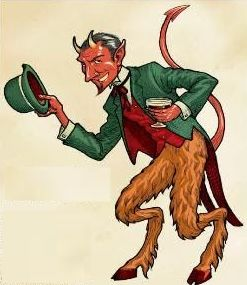
\includegraphics[max height = 0.3\textheight]{Images/devil.jpg}
    }{}

    \vspace*{.9em}
    Please mute yourselves!
    \end{center}


    \vfill
  \end{frame}
}

\AtBeginSubsection[]{
  \begin{frame}
    \vfill
    \centering
    \begin{beamercolorbox}[sep=8pt,center,shadow=true,rounded=true]{title}
    \usebeamerfont{title}\insertsectionhead\par%
    \usebeamerfont{subtitle}\insertsubsectionhead\par%
    \end{beamercolorbox}
    \ifthenelse{\equal{\subsecname}{Answers}} {
        \begin{center}
        Unmute yourselves!
        \end{center}
    }
    \vfill
  \end{frame}
}
\begin{document}

\title{Welcome to Quarantine Trivia XVI!}
\date{}

\begin{frame}
\titlepage{}
\begin{center}

\includegraphics[max width=0.9\textwidth,
    max height=0.4\textheight]{Images/triviatitleframelogo.png}
\end{center}
\end{frame}

\begin{frame}
Welcome to the Spring edition of Quarantine Trivia!
\pause
\begin{center}
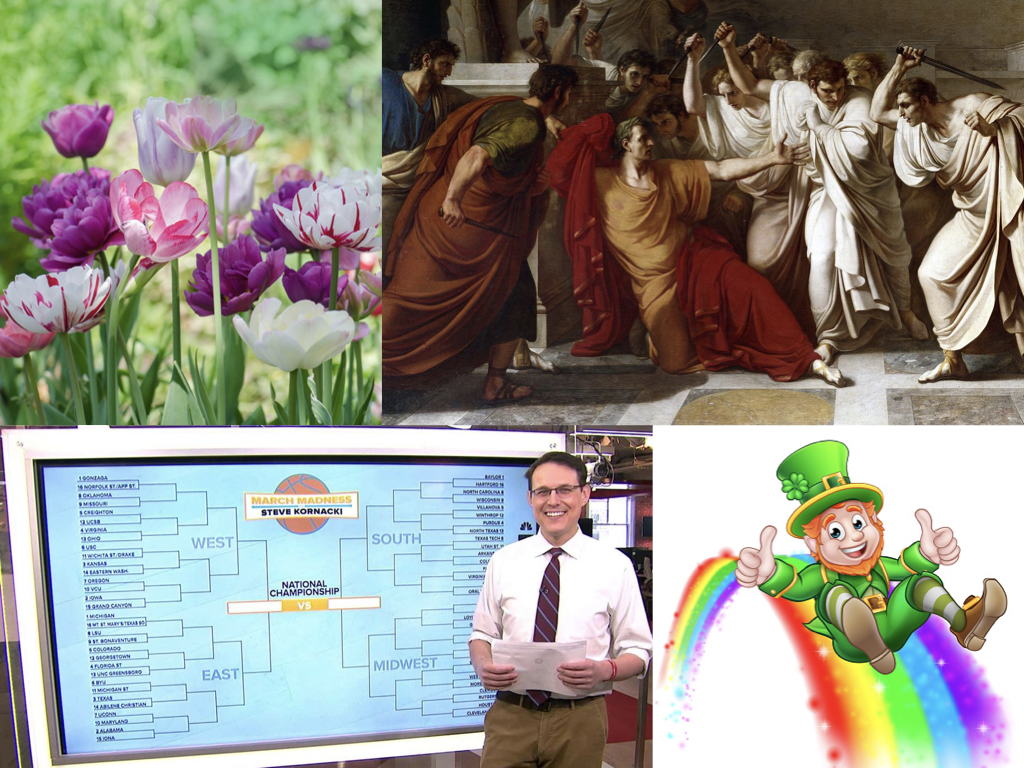
\includegraphics[max width=\textwidth,max height=\textheight]{Images/march.jpg}
\end{center}
\end{frame}

\begingroup{}
\begingroup{}
\begin{frame}[t]{Categories}
This week, you'll be answering questions in the following categories:
\begin{enumerate}
\item Earth, Wind \& Fire (featuring Water)
\item Units of Measure
\item As Seen on TV
\item Spring
\item Portmanteaus
\item ``Colorful'' People
\item Booze Clues
\item NPR and PBS
\item Tales and Fables
\item Ciao for Now
\item Bonus Round
\end{enumerate}
\end{frame}
\endgroup{}

\begingroup{}
\begin{frame}
\vfill{}
\begin{beamercolorbox}[sep=8pt,center,shadow=true,rounded=true]{title}
\usebeamerfont{title}Good luck everyone! And have fun!
\end{beamercolorbox}
\vfill{}
\end{frame}
\endgroup{}
\def\thisSectionName{Earth, Wind \& Fire (featuring Water)}
\section{Round 1}
\subsection*{Q1}
\begin{frame}[t]{Round 1 --- Earth, Wind \& Fire (featuring Water) --- \mbox{Question 1}}
\vspace{-0.5em}
\begin{block}{Question}
Who was the author of \emph{Fahrenheit 451}, in which ``firemen'' burn books?
\end{block}
\end{frame}
\subsection*{Q2}
\begin{frame}[t]{Round 1 --- Earth, Wind \& Fire (featuring Water) --- \mbox{Question 2}}
\vspace{-0.5em}
\begin{block}{Question}
Which meteorological phenomena give rise to the lowest observed sea-level atmospheric pressures?
\end{block}
\end{frame}
\subsection*{Q3}
\begin{frame}[t]{Round 1 --- Earth, Wind \& Fire (featuring Water) --- \mbox{Question 3}}
\vspace{-0.5em}
\begin{block}{Question}
To within 3\%, what percent of the Earth's surface is covered in water?
\end{block}
\end{frame}
\subsection*{Q4}
\begin{frame}[t]{Round 1 --- Earth, Wind \& Fire (featuring Water) --- \mbox{Question 4}}
\vspace{-0.5em}
\begin{block}{Question}
The center of the Earth is very hot. About half of this heat is left over from the formation of the Earth itself; the other half is continuously produced by what process?
\end{block}
\end{frame}
\subsection*{Q5}
\begin{frame}[t]{Round 1 --- Earth, Wind \& Fire (featuring Water) --- \mbox{Question 5}}
\vspace{-0.5em}
\begin{block}{Question}
By volume, what is the third most abundant gas  in Earth's atmosphere? (It comes after nitrogen (78\%) and oxygen (21\%).)
\end{block}
\end{frame}
\subsection*{Q6}
\begin{frame}[t]{Round 1 --- Earth, Wind \& Fire (featuring Water) --- \mbox{Question 6}}
\vspace{-0.5em}
\begin{block}{Question}
Who is the first person mentioned in the Billy Joel song ``We Didn't Start the Fire''? (The person's first name and last name are the first two words of the song.)
\end{block}
\end{frame}
\subsection*{Q7}
\begin{frame}[t]{Round 1 --- Earth, Wind \& Fire (featuring Water) --- \mbox{Question 7}}
\vspace{-0.5em}
\begin{columns}[T,totalwidth=\linewidth]
\begin{column}{0.32\linewidth}
\begin{block}{Question}
What is the name of the flame-producing piece of lab equipment pictured here? (You may have used one in your high school chemistry class.)
\end{block}
\end{column}
\begin{column}{0.65\linewidth}
\begin{center}
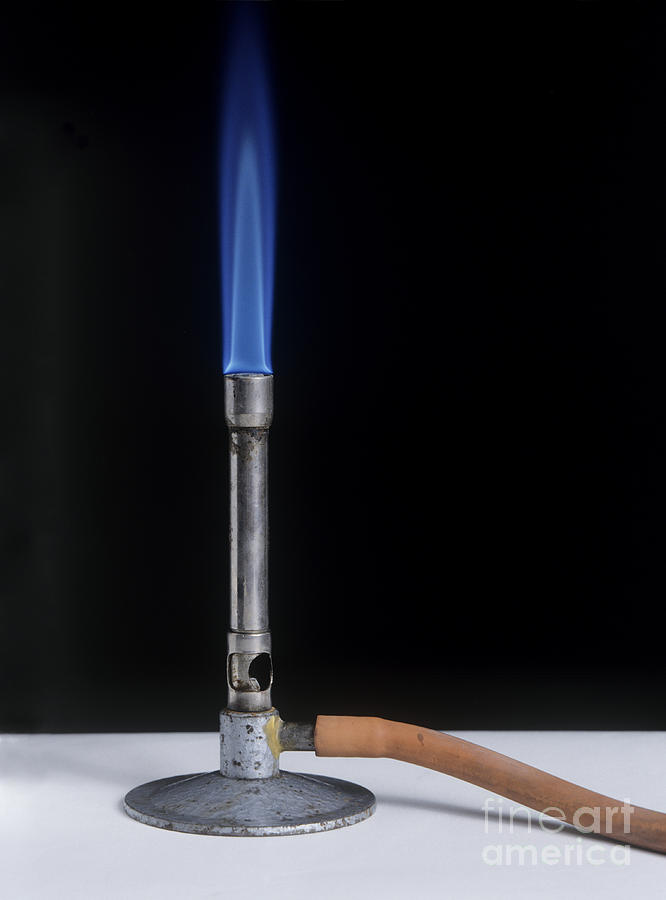
\includegraphics[max width=0.95\textwidth,max height=0.7\textheight]{{Images/bunsen}.jpeg}
\end{center}
\end{column}
\end{columns}
\end{frame}
\subsection*{Q8}
\begin{frame}[t]{Round 1 --- Earth, Wind \& Fire (featuring Water) --- \mbox{Question 8}}
\vspace{-0.5em}
\begin{block}{Question}
The majority of the nutrient-rich dust that nourishes the Amazon rainforest is carried by wind from which desert?
\end{block}
\end{frame}
\subsection*{Q9}
\begin{frame}[t]{Round 1 --- Earth, Wind \& Fire (featuring Water) --- \mbox{Question 9}}
\vspace{-0.5em}
\begin{block}{Question}
Which early species of man (genus \emph{homo}) is generally considered the first to have controlled fire?
\end{block}
\end{frame}
\subsection*{Q10}
\begin{frame}[t]{Round 1 --- Earth, Wind \& Fire (featuring Water) --- \mbox{Question 10}}
\vspace{-0.5em}
\begin{block}{Question}
When water freezes to form ice, its molecules form a crystalline structure that exhibits what kind of symmetry? (The answer relates to a number.)
\end{block}
\end{frame}
\subsection{Answers}
\begin{frame}[t]{Round 1 --- Earth, Wind \& Fire (featuring Water) --- \mbox{Answer 1}}
\vspace{-0.5em}
\begin{block}{Question}
Who was the author of \emph{Fahrenheit 451}, in which ``firemen'' burn books?
\end{block}

\visible<2->{
    \begin{columns}[T,totalwidth=\linewidth]
    \begin{column}{0.32\linewidth}
    \begin{block}{Answer}
    Ray Bradbury
    \end{block}
    \end{column}
    \begin{column}{0.65\linewidth}
    \begin{center}
    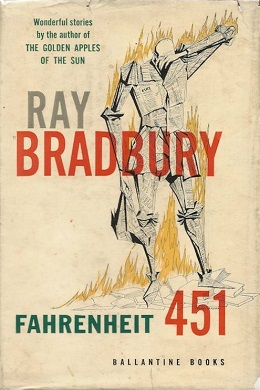
\includegraphics[max height=.45\textheight,
        max width=0.95\textwidth]{{Images/far451}.jpg}
    \end{center}
    \end{column}
    \end{columns}
}
\end{frame}
\begin{frame}[t]{Round 1 --- Earth, Wind \& Fire (featuring Water) --- \mbox{Answer 2}}
\vspace{-0.5em}
\begin{block}{Question}
Which meteorological phenomena give rise to the lowest observed sea-level atmospheric pressures?
\end{block}

\visible<2->{
    \begin{columns}[T,totalwidth=\linewidth]
    \begin{column}{0.32\linewidth}
    \begin{block}{Answer}
    Hurricanes / cyclones / typhoons (the air pressure in the eye of a hurricane can be up to 15\% lower than the surrounding air pressure)
    \end{block}
    \end{column}
    \begin{column}{0.65\linewidth}
    \begin{center}
    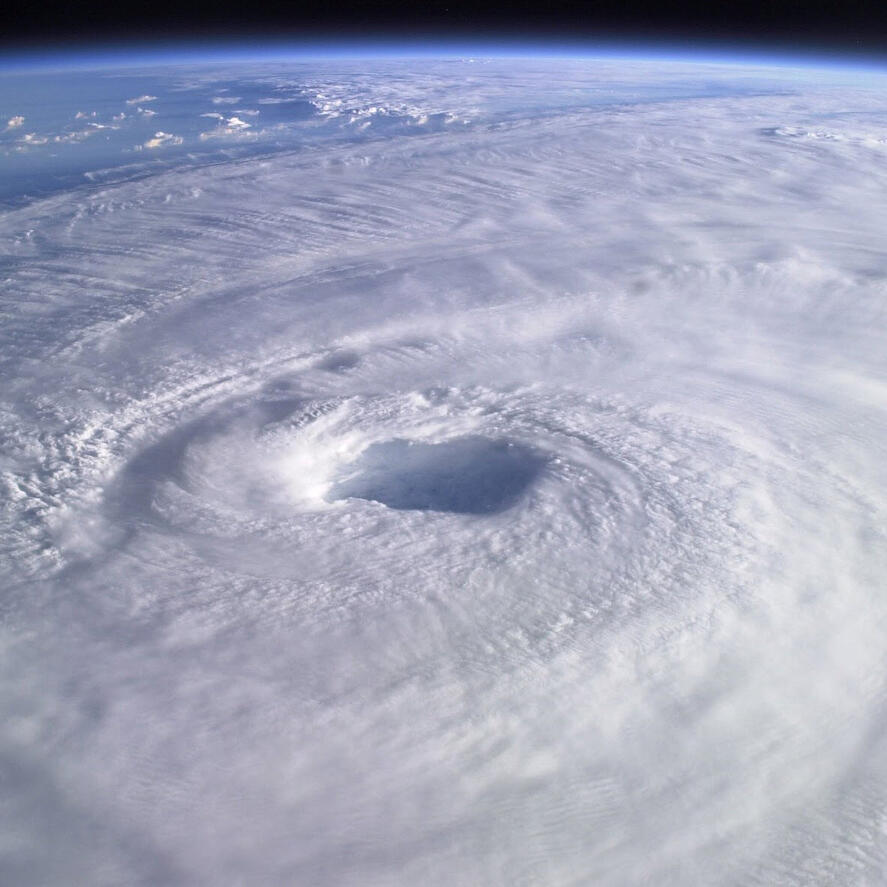
\includegraphics[max height=.45\textheight,
        max width=0.95\textwidth]{{Images/hurricane}.jpg}
    \end{center}
    \end{column}
    \end{columns}
}
\end{frame}
\begin{frame}[t]{Round 1 --- Earth, Wind \& Fire (featuring Water) --- \mbox{Answer 3}}
\vspace{-0.5em}
\begin{block}{Question}
To within 3\%, what percent of the Earth's surface is covered in water?
\end{block}

\visible<2->{
    \begin{columns}[T,totalwidth=\linewidth]
    \begin{column}{0.32\linewidth}
    \begin{block}{Answer}
    71\% (68\%-74\% will be accepted)
    \end{block}
    \end{column}
    \begin{column}{0.65\linewidth}
    \begin{center}
    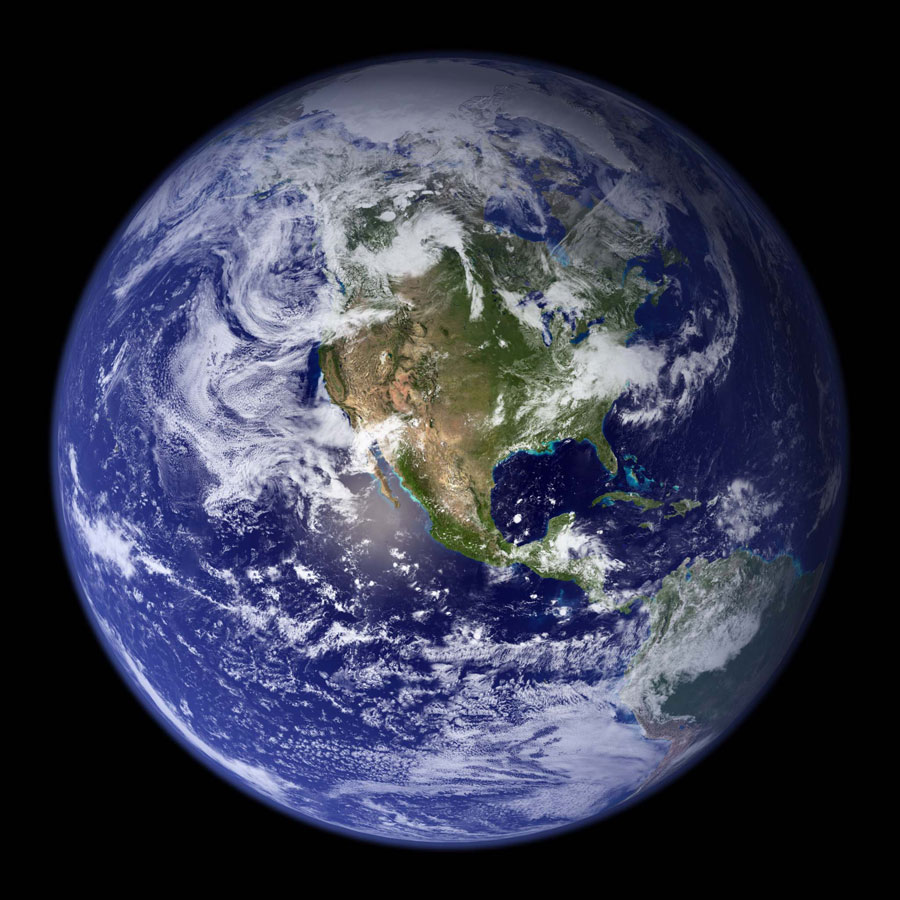
\includegraphics[max height=.45\textheight,
        max width=0.95\textwidth]{{Images/earth}.jpeg}
    \end{center}
    \end{column}
    \end{columns}
}
\end{frame}
\begin{frame}[t]{Round 1 --- Earth, Wind \& Fire (featuring Water) --- \mbox{Answer 4}}
\vspace{-0.5em}
\begin{block}{Question}
The center of the Earth is very hot. About half of this heat is left over from the formation of the Earth itself; the other half is continuously produced by what process?
\end{block}

\visible<2->{
    \begin{columns}[T,totalwidth=\linewidth]
    \begin{column}{0.32\linewidth}
    \begin{block}{Answer}
    Radiation / radioactivity / radioactive decay
    \end{block}
    \end{column}
    \begin{column}{0.65\linewidth}
    \begin{center}
    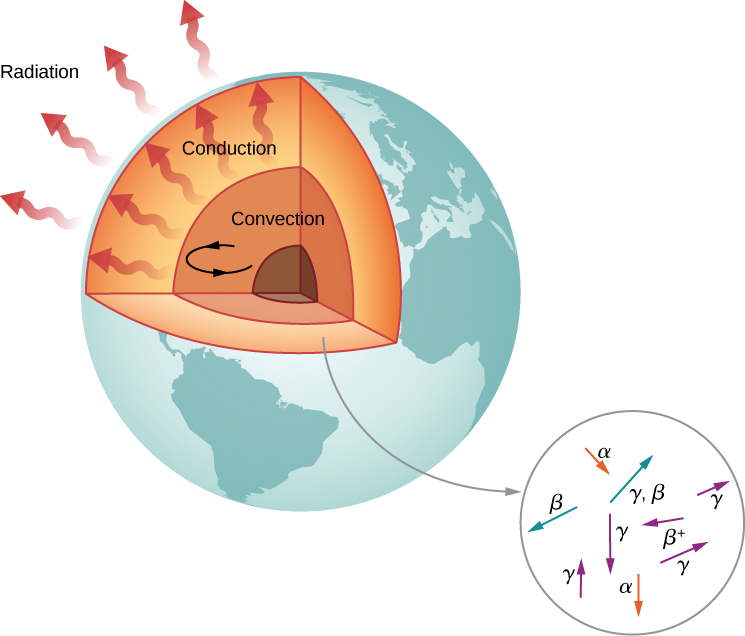
\includegraphics[max height=.45\textheight,
        max width=0.95\textwidth]{{Images/earthcore}.jpg}
    \end{center}
    \end{column}
    \end{columns}
}
\end{frame}
\begin{frame}[t]{Round 1 --- Earth, Wind \& Fire (featuring Water) --- \mbox{Answer 5}}
\vspace{-0.5em}
\begin{block}{Question}
By volume, what is the third most abundant gas  in Earth's atmosphere? (It comes after nitrogen (78\%) and oxygen (21\%).)
\end{block}

\visible<2->{
    \begin{columns}[T,totalwidth=\linewidth]
    \begin{column}{0.32\linewidth}
    \begin{block}{Answer}
    Argon (0.93\%)
    \end{block}
    \end{column}
    \begin{column}{0.65\linewidth}
    \begin{center}
    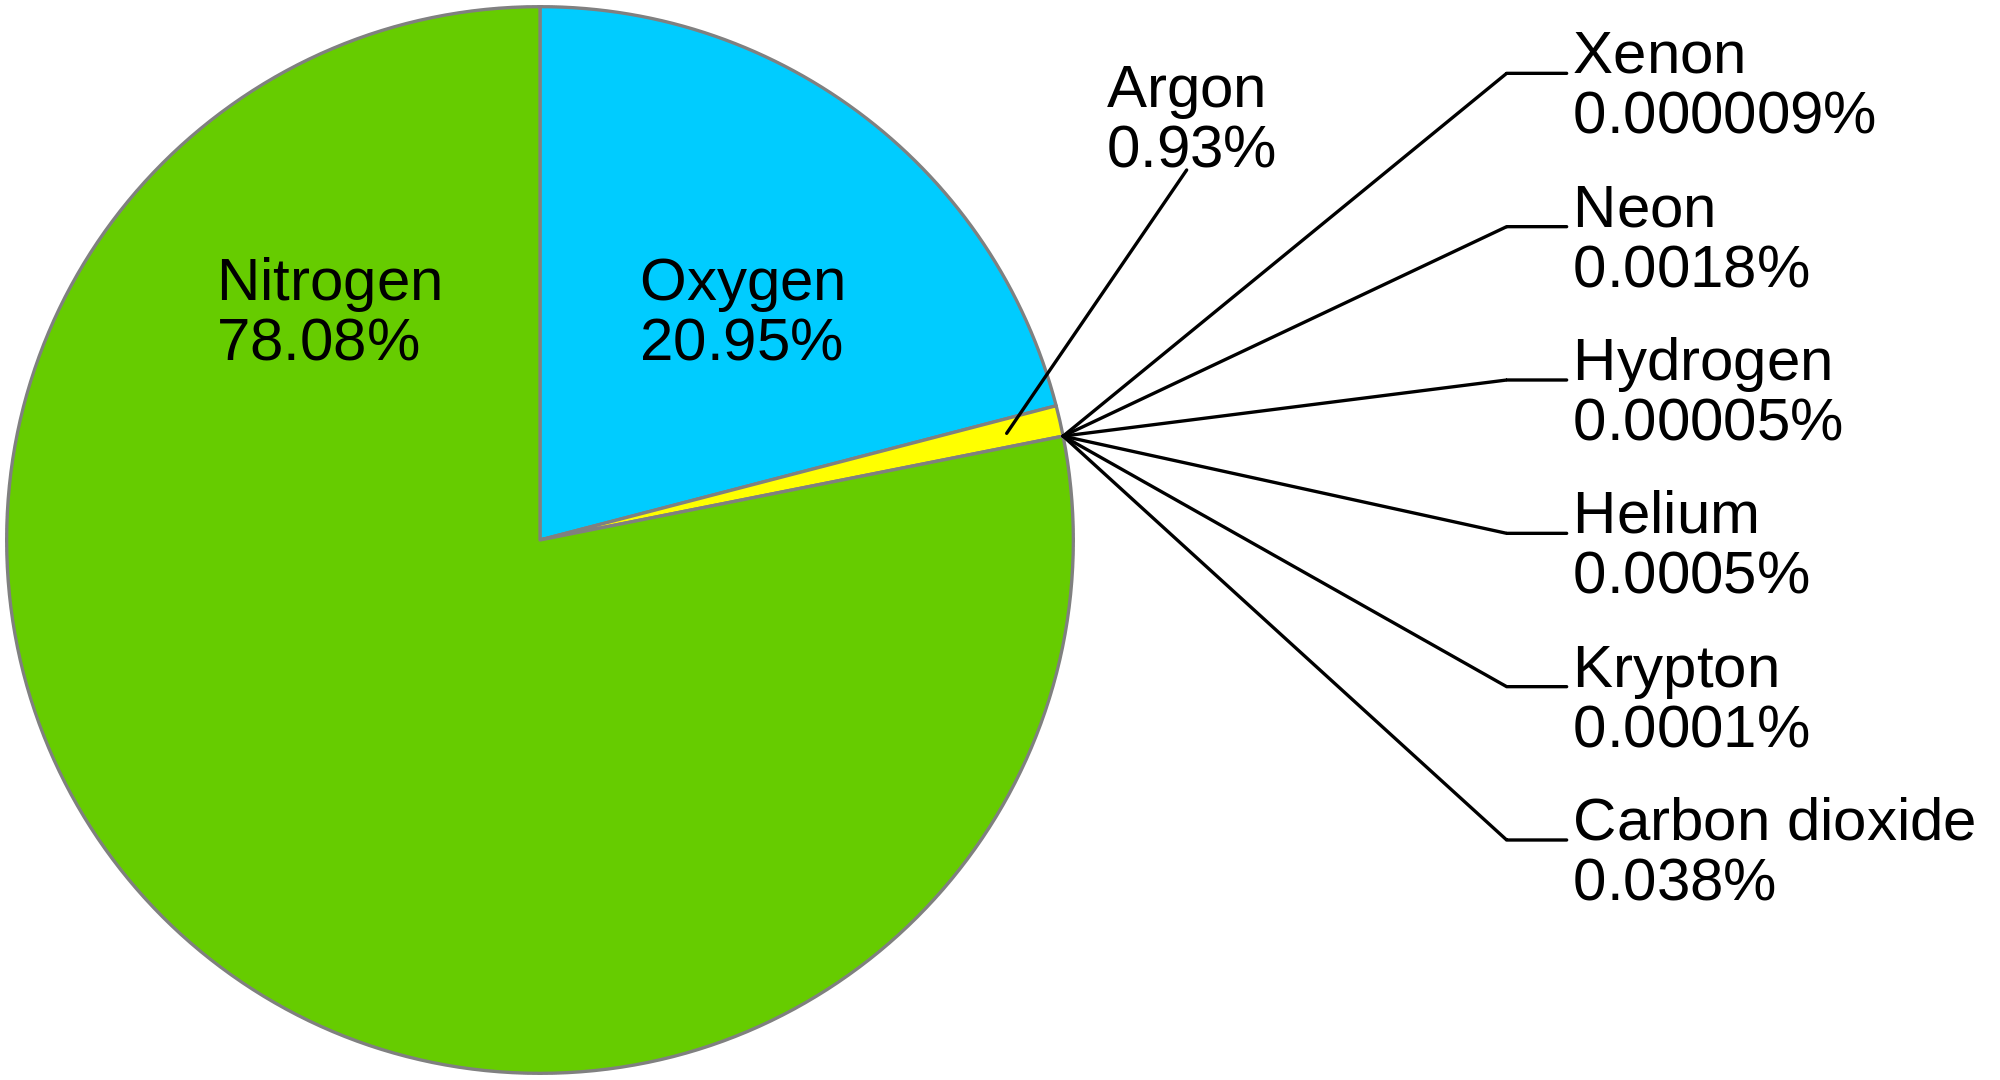
\includegraphics[max height=.45\textheight,
        max width=0.95\textwidth]{{Images/argon}.png}
    \end{center}
    \end{column}
    \end{columns}
}
\end{frame}
\begin{frame}[t]{Round 1 --- Earth, Wind \& Fire (featuring Water) --- \mbox{Answer 6}}
\vspace{-0.5em}
\begin{block}{Question}
Who is the first person mentioned in the Billy Joel song ``We Didn't Start the Fire''? (The person's first name and last name are the first two words of the song.)
\end{block}

\visible<2->{
    \begin{columns}[T,totalwidth=\linewidth]
    \begin{column}{0.32\linewidth}
    \begin{block}{Answer}
    Harry Truman
    \end{block}
    \end{column}
    \begin{column}{0.65\linewidth}
    \begin{center}
    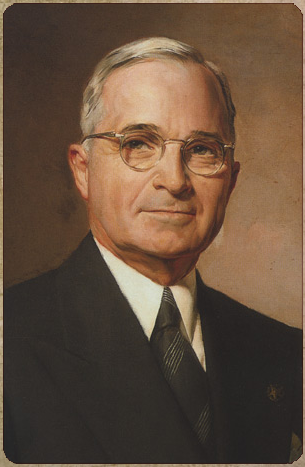
\includegraphics[max height=.45\textheight,
        max width=0.95\textwidth]{{Images/truman}.jpg}
    \end{center}
    \end{column}
    \end{columns}
}
\end{frame}
\begin{frame}[t]{Round 1 --- Earth, Wind \& Fire (featuring Water) --- \mbox{Answer 7}}
\vspace{-0.5em}
\begin{columns}[T,totalwidth=\linewidth]
\begin{column}{0.32\linewidth}
\begin{block}{Question}
What is the name of the flame-producing piece of lab equipment pictured here? (You may have used one in your high school chemistry class.)
\end{block}
\visible<2->{
    \begin{block}{Answer}
    Bunsen burner
    \end{block}
}
\end{column}
\begin{column}{0.65\linewidth}
\begin{center}
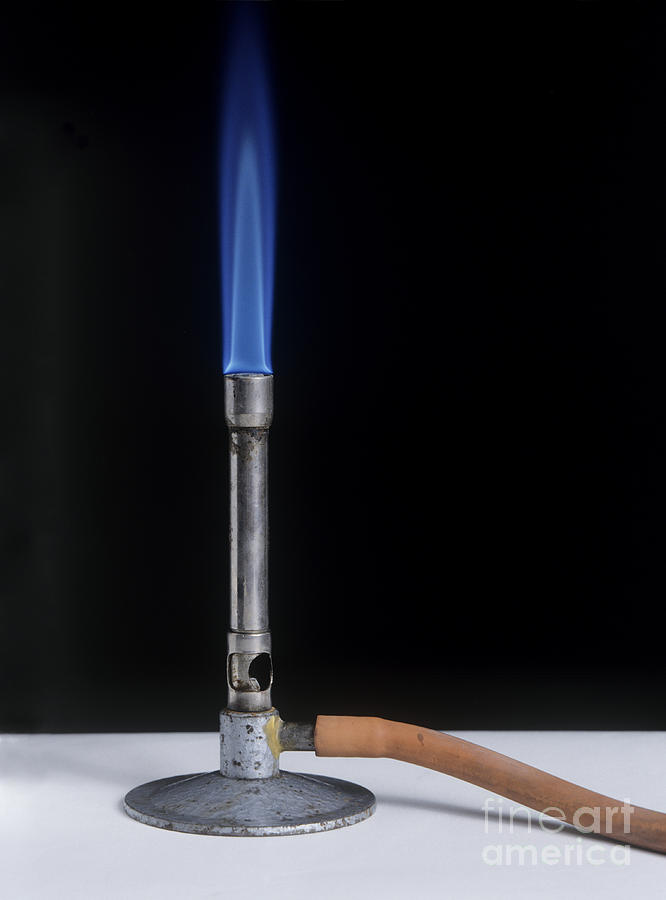
\includegraphics[max width=0.95\textwidth,max height=0.7\textheight]{{Images/bunsen}.jpeg}
\end{center}
\end{column}
\end{columns}
\end{frame}
\begin{frame}[t]{Round 1 --- Earth, Wind \& Fire (featuring Water) --- \mbox{Answer 8}}
\vspace{-0.5em}
\begin{block}{Question}
The majority of the nutrient-rich dust that nourishes the Amazon rainforest is carried by wind from which desert?
\end{block}

\visible<2->{
    \begin{columns}[T,totalwidth=\linewidth]
    \begin{column}{0.32\linewidth}
    \begin{block}{Answer}
    The Sahara
    \end{block}
    \end{column}
    \begin{column}{0.65\linewidth}
    \begin{center}
    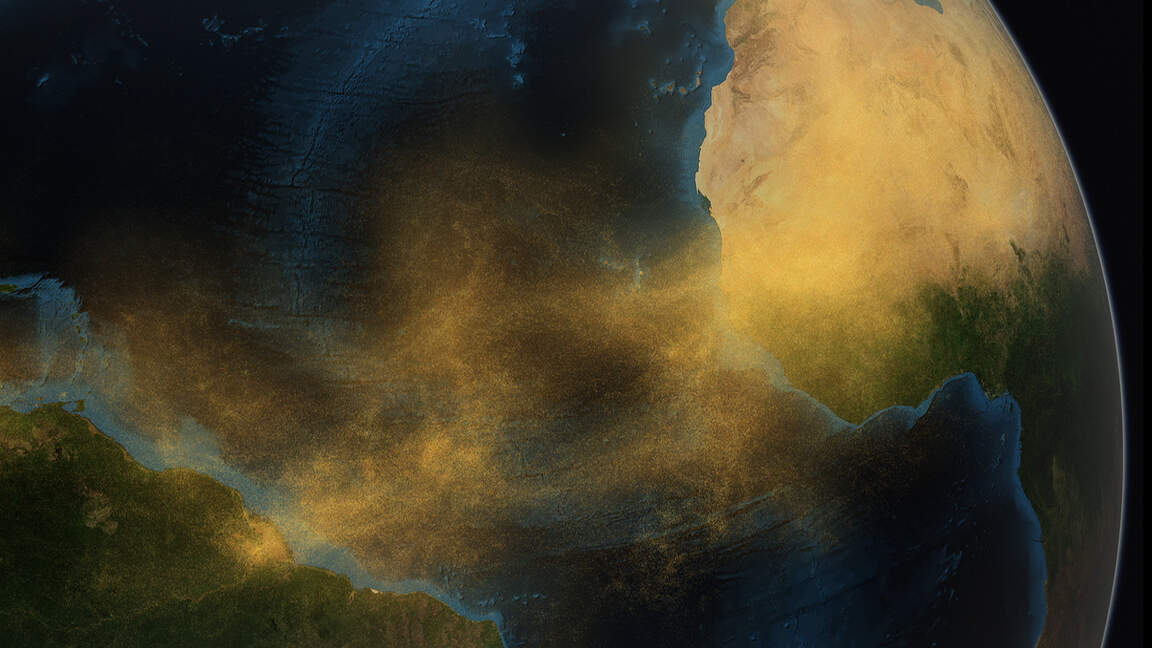
\includegraphics[max height=.45\textheight,
        max width=0.95\textwidth]{{Images/sahara}.jpg}
    \end{center}
    \end{column}
    \end{columns}
}
\end{frame}
\begin{frame}[t]{Round 1 --- Earth, Wind \& Fire (featuring Water) --- \mbox{Answer 9}}
\vspace{-0.5em}
\begin{block}{Question}
Which early species of man (genus \emph{homo}) is generally considered the first to have controlled fire?
\end{block}

\visible<2->{
    \begin{columns}[T,totalwidth=\linewidth]
    \begin{column}{0.32\linewidth}
    \begin{block}{Answer}
    \emph{Homo erectus}
    \end{block}
    \end{column}
    \begin{column}{0.65\linewidth}
    \begin{center}
    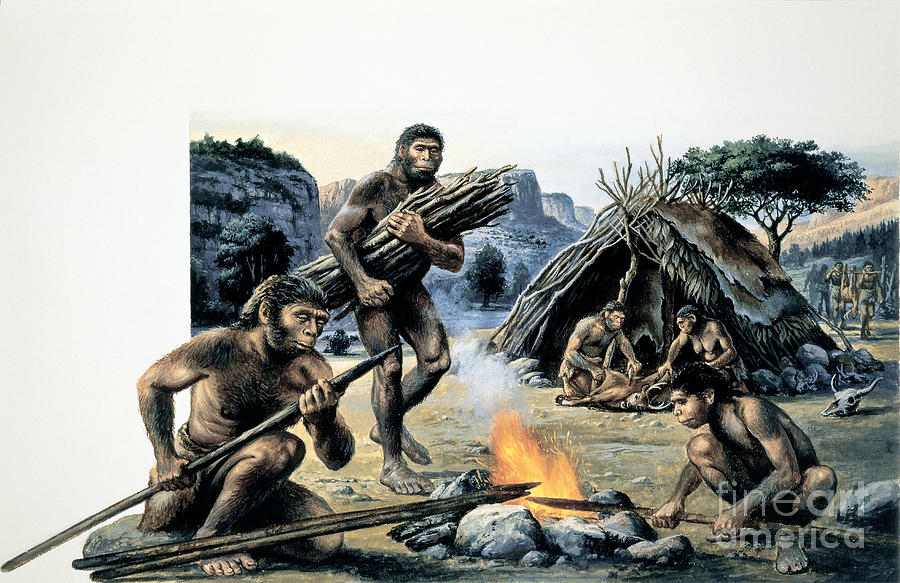
\includegraphics[max height=.45\textheight,
        max width=0.95\textwidth]{{Images/erectus}.jpg}
    \end{center}
    \end{column}
    \end{columns}
}
\end{frame}
\begin{frame}[t]{Round 1 --- Earth, Wind \& Fire (featuring Water) --- \mbox{Answer 10}}
\vspace{-0.5em}
\begin{block}{Question}
When water freezes to form ice, its molecules form a crystalline structure that exhibits what kind of symmetry? (The answer relates to a number.)
\end{block}

\visible<2->{
    \begin{columns}[T,totalwidth=\linewidth]
    \begin{column}{0.32\linewidth}
    \begin{block}{Answer}
    Hexagonal / sixfold / six-sided
    \end{block}
    \end{column}
    \begin{column}{0.65\linewidth}
    \begin{center}
    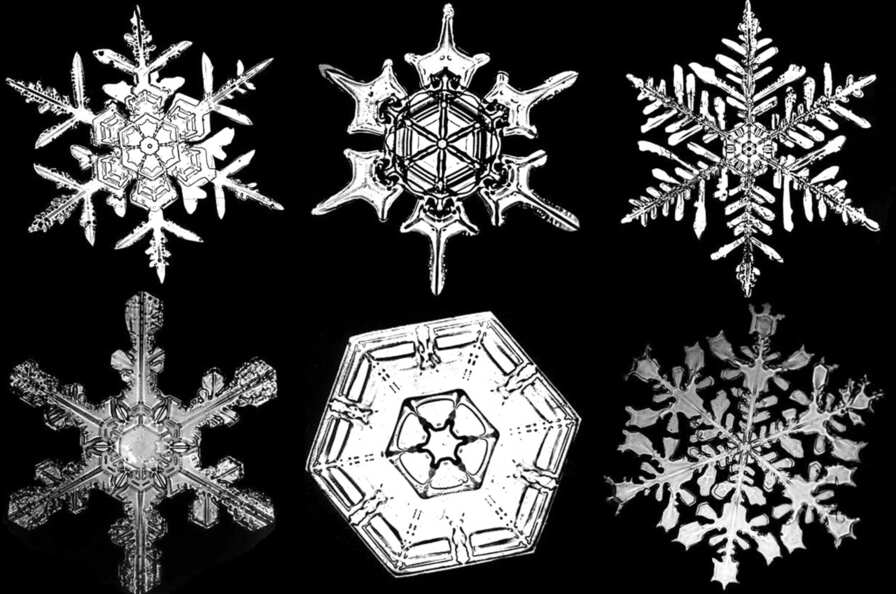
\includegraphics[max height=.45\textheight,
        max width=0.95\textwidth]{{Images/snowflake}.jpg}
    \end{center}
    \end{column}
    \end{columns}
}
\end{frame}
\def\thisSectionName{Units of Measure}
\section{Round 2}
\subsection*{Q1}
\begin{frame}[t]{Round 2 --- Units of Measure --- \mbox{Question 1}}
\vspace{-0.5em}
\begin{block}{Question}
In 1799, which country became the first country to adopt the metric system?
\end{block}
\end{frame}
\subsection*{Q2}
\begin{frame}[t]{Round 2 --- Units of Measure --- \mbox{Question 2}}
\vspace{-0.5em}
\begin{block}{Question}
How many US gallons are in a barrel of oil?
\end{block}
\end{frame}
\subsection*{Q3}
\begin{frame}[t]{Round 2 --- Units of Measure --- \mbox{Question 3}}
\vspace{-0.5em}
\begin{block}{Question}
A calorie (lowercased) is the amount of energy it takes to raise the temperature of what mass of water by \SI{1}{\celsius}?
\end{block}
\end{frame}
\subsection*{Q4}
\begin{frame}[t]{Round 2 --- Units of Measure --- \mbox{Question 4}}
\vspace{-0.5em}
\begin{block}{Question}
In chemistry, what is the name of the constant that is equal to the number of particles in a mole of a particular substance?
\end{block}
\end{frame}
\subsection*{Q5}
\begin{frame}[t]{Round 2 --- Units of Measure --- \mbox{Question 5}}
\vspace{-0.5em}
\begin{block}{Question}
In units of cubits, give any one of the length, width, or height of Noah's Ark as described in the Bible in Genesis 6:15.
\end{block}
\end{frame}
\subsection*{Q6}
\begin{frame}[t]{Round 2 --- Units of Measure --- \mbox{Question 6}}
\vspace{-0.5em}
\begin{block}{Question}
What is the name of the temperature scale on which zero degrees corresponds to absolute zero and whose degrees have a magnitude of \SI{1}{\celsius}?
\end{block}
\end{frame}
\subsection*{Q7}
\begin{frame}[t]{Round 2 --- Units of Measure --- \mbox{Question 7}}
\vspace{-0.5em}
\begin{block}{Question}
The meter was originally defined so that what feature of the Earth had a length of 10 million meters?
\end{block}
\end{frame}
\subsection*{Q8}
\begin{frame}[t]{Round 2 --- Units of Measure --- \mbox{Question 8}}
\vspace{-0.5em}
\begin{block}{Question}
How many furlongs are in a mile? (The answer is a whole number.)
\end{block}
\end{frame}
\subsection*{Q9}
\begin{frame}[t]{Round 2 --- Units of Measure --- \mbox{Question 9}}
\vspace{-0.5em}
\begin{block}{Question}
How many feet are in a fathom? (The answer is a whole number.)
\end{block}
\end{frame}
\subsection*{Q10}
\begin{frame}[t]{Round 2 --- Units of Measure --- \mbox{Question 10}}
\vspace{-0.5em}
\begin{block}{Question}
As of 2019, all SI (International System of Units) base units are defined in terms of fundamental physical constants and the behavior of photons and atoms. Which unit of measure was the last SI base unit to be defined by  a physical object?
\end{block}
\end{frame}
\subsection{Answers}
\begin{frame}[t]{Round 2 --- Units of Measure --- \mbox{Answer 1}}
\vspace{-0.5em}
\begin{block}{Question}
In 1799, which country became the first country to adopt the metric system?
\end{block}

\visible<2->{
    \begin{columns}[T,totalwidth=\linewidth]
    \begin{column}{0.32\linewidth}
    \begin{block}{Answer}
    France
    \end{block}
    \end{column}
    \begin{column}{0.65\linewidth}
    \begin{center}
    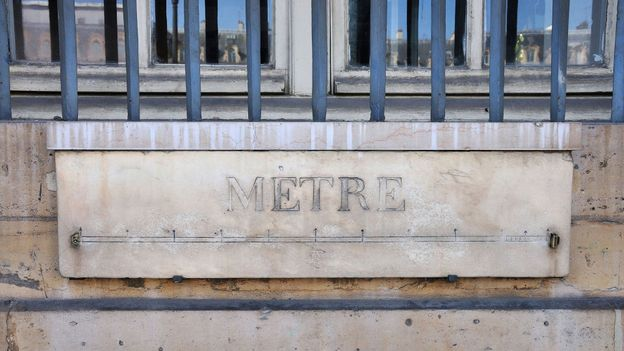
\includegraphics[max height=.45\textheight,
        max width=0.95\textwidth]{{Images/metre}.jpg}
    \end{center}
    \end{column}
    \end{columns}
}
\end{frame}
\begin{frame}[t]{Round 2 --- Units of Measure --- \mbox{Answer 2}}
\vspace{-0.5em}
\begin{block}{Question}
How many US gallons are in a barrel of oil?
\end{block}

\visible<2->{
    \begin{columns}[T,totalwidth=\linewidth]
    \begin{column}{0.32\linewidth}
    \begin{block}{Answer}
    42
    \end{block}
    \end{column}
    \begin{column}{0.65\linewidth}
    \begin{center}
    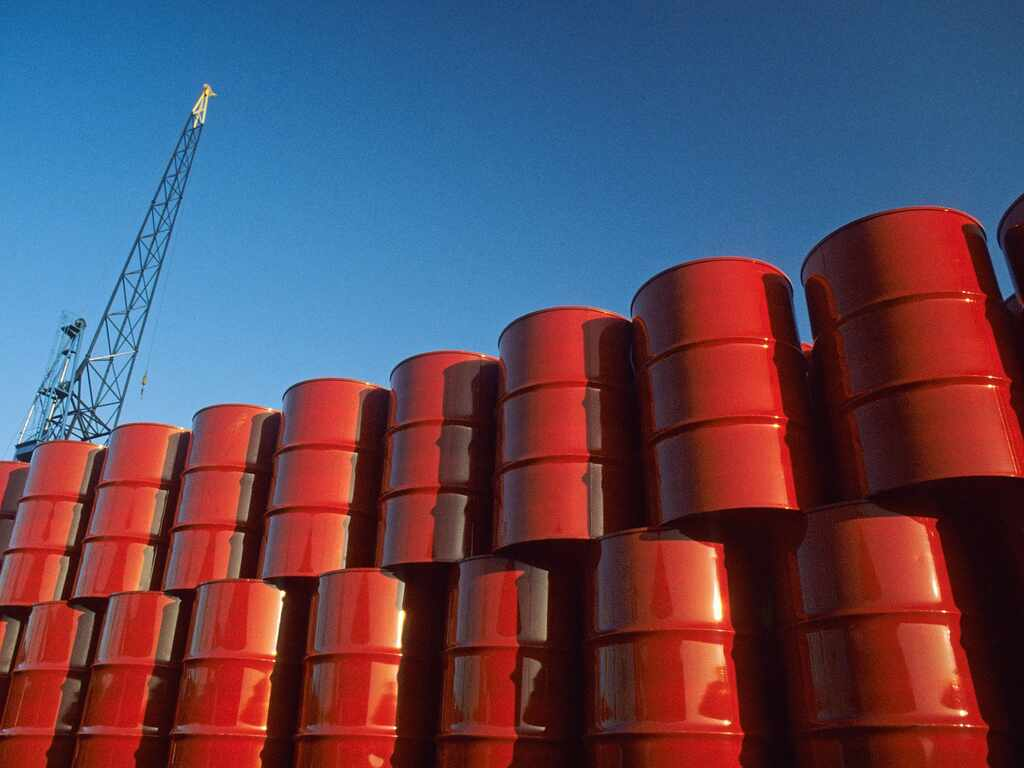
\includegraphics[max height=.45\textheight,
        max width=0.95\textwidth]{{Images/barreloil}.jpg}
    \end{center}
    \end{column}
    \end{columns}
}
\end{frame}
\begin{frame}[t]{Round 2 --- Units of Measure --- \mbox{Answer 3}}
\vspace{-0.5em}
\begin{block}{Question}
A calorie (lowercased) is the amount of energy it takes to raise the temperature of what mass of water by \SI{1}{\celsius}?
\end{block}

\visible<2->{
    \begin{columns}[T,totalwidth=\linewidth]
    \begin{column}{0.32\linewidth}
    \begin{block}{Answer}
    1 gram
    \end{block}
    \end{column}
    \begin{column}{0.65\linewidth}
    \begin{center}
    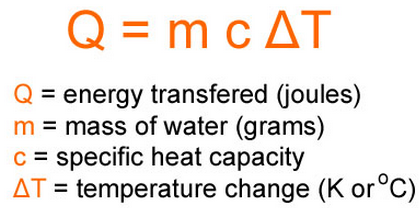
\includegraphics[max height=.45\textheight,
        max width=0.95\textwidth]{{Images/specificheat}.png}
    \end{center}
    \end{column}
    \end{columns}
}
\end{frame}
\begin{frame}[t]{Round 2 --- Units of Measure --- \mbox{Answer 4}}
\vspace{-0.5em}
\begin{block}{Question}
In chemistry, what is the name of the constant that is equal to the number of particles in a mole of a particular substance?
\end{block}

\visible<2->{
    \begin{columns}[T,totalwidth=\linewidth]
    \begin{column}{0.32\linewidth}
    \begin{block}{Answer}
    Avogadro's constant / Avogadro's number
    \end{block}
    \end{column}
    \begin{column}{0.65\linewidth}
    \begin{center}
    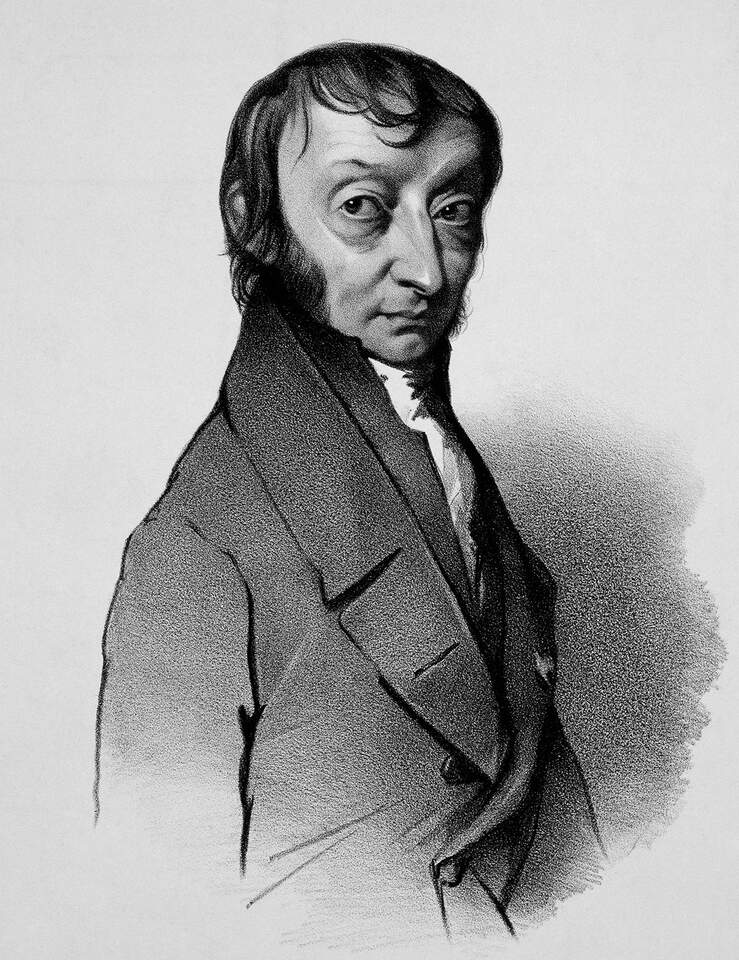
\includegraphics[max height=.45\textheight,
        max width=0.95\textwidth]{{Images/avogadro}.jpg}
    \end{center}
    \end{column}
    \end{columns}
}
\end{frame}
\begin{frame}[t]{Round 2 --- Units of Measure --- \mbox{Answer 5}}
\vspace{-0.5em}
\begin{block}{Question}
In units of cubits, give any one of the length, width, or height of Noah's Ark as described in the Bible in Genesis 6:15.
\end{block}

\visible<2->{
    \begin{columns}[T,totalwidth=\linewidth]
    \begin{column}{0.32\linewidth}
    \begin{block}{Answer}
    Three hundred cubits long, fifty cubits wide, and thirty cubits high (we only needed one)
    \end{block}
    \end{column}
    \begin{column}{0.65\linewidth}
    \begin{center}
    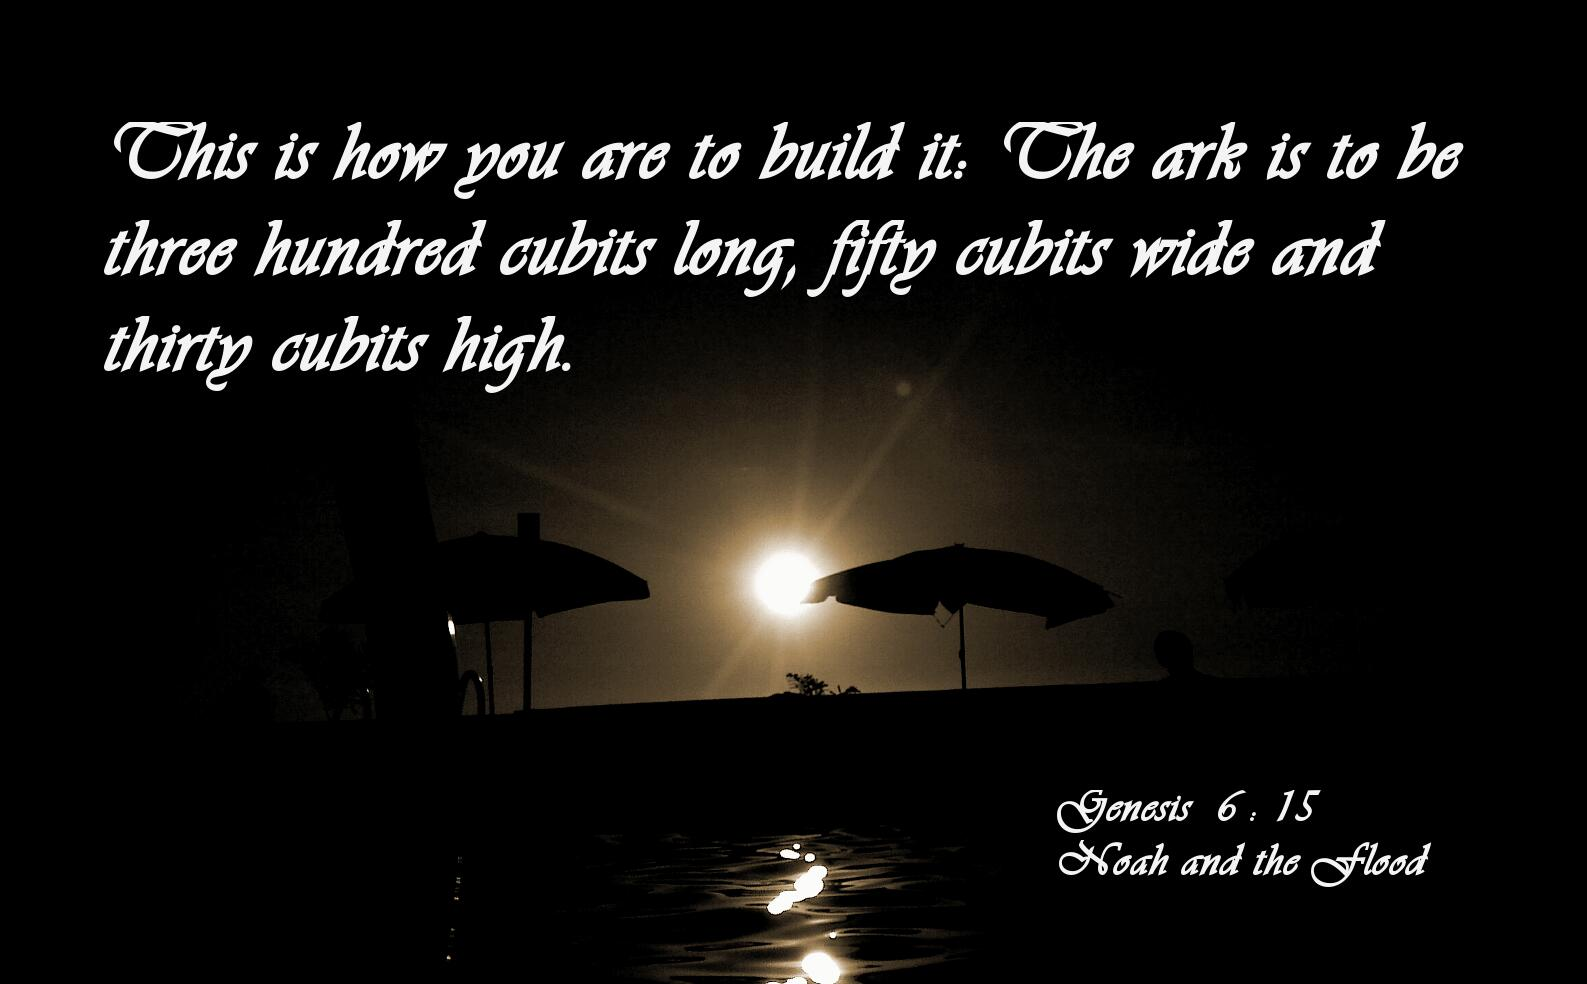
\includegraphics[max height=.45\textheight,
        max width=0.95\textwidth]{{Images/genesis615}.jpg}
    \end{center}
    \end{column}
    \end{columns}
}
\end{frame}
\begin{frame}[t]{Round 2 --- Units of Measure --- \mbox{Answer 6}}
\vspace{-0.5em}
\begin{block}{Question}
What is the name of the temperature scale on which zero degrees corresponds to absolute zero and whose degrees have a magnitude of \SI{1}{\celsius}?
\end{block}

\visible<2->{
    \begin{columns}[T,totalwidth=\linewidth]
    \begin{column}{0.32\linewidth}
    \begin{block}{Answer}
    Kelvin
    \end{block}
    \end{column}
    \begin{column}{0.65\linewidth}
    \begin{center}
    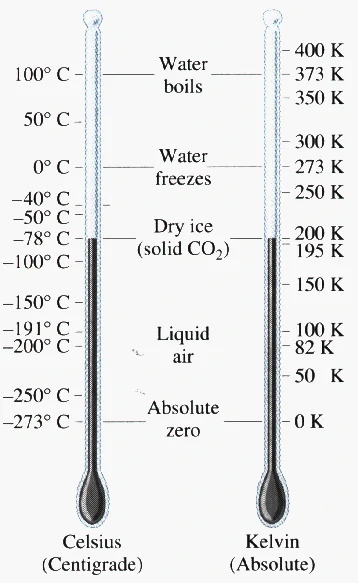
\includegraphics[max height=.45\textheight,
        max width=0.95\textwidth]{{Images/kelvin}.jpg}
    \end{center}
    \end{column}
    \end{columns}
}
\end{frame}
\begin{frame}[t]{Round 2 --- Units of Measure --- \mbox{Answer 7}}
\vspace{-0.5em}
\begin{block}{Question}
The meter was originally defined so that what feature of the Earth had a length of 10 million meters?
\end{block}

\visible<2->{
    \begin{columns}[T,totalwidth=\linewidth]
    \begin{column}{0.6\linewidth}
    \begin{block}{Answer}
    The distance between the equator and the poles (we'll also accept ``one-quarter of the circumference'' although that isn't precise due to the fact that the Earth is not a perfect sphere)
    \end{block}
    \end{column}
    \begin{column}{0.38\linewidth}
    \begin{center}
    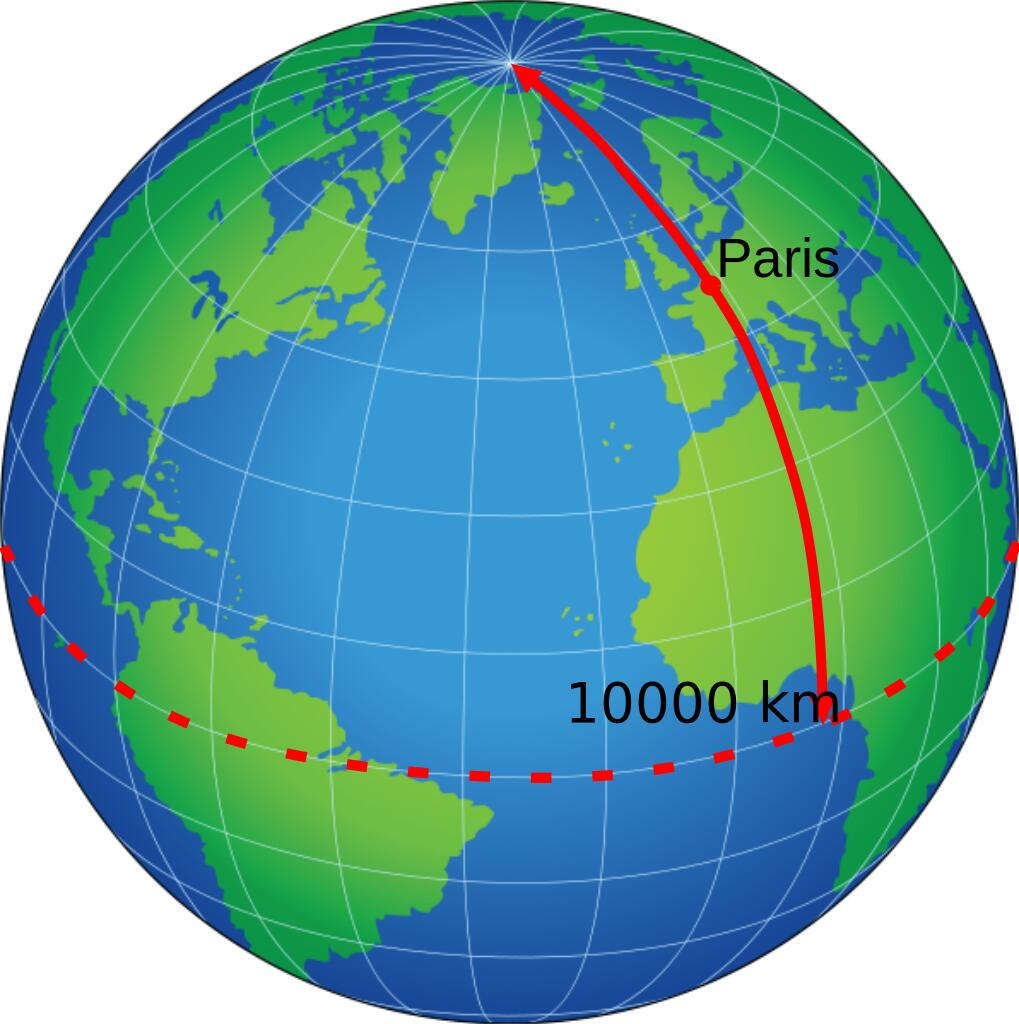
\includegraphics[max width=0.95\textwidth,
        max height=0.48000\textheight]{{Images/meterdef}.jpg}
    \end{center}
    \end{column}
    \end{columns}
}
\end{frame}
\begin{frame}[t]{Round 2 --- Units of Measure --- \mbox{Answer 8}}
\vspace{-0.5em}
\begin{block}{Question}
How many furlongs are in a mile? (The answer is a whole number.)
\end{block}

\visible<2->{
    \begin{columns}[T,totalwidth=\linewidth]
    \begin{column}{0.32\linewidth}
    \begin{block}{Answer}
    Eight
    \end{block}
    \end{column}
    \begin{column}{0.65\linewidth}
    \begin{center}
    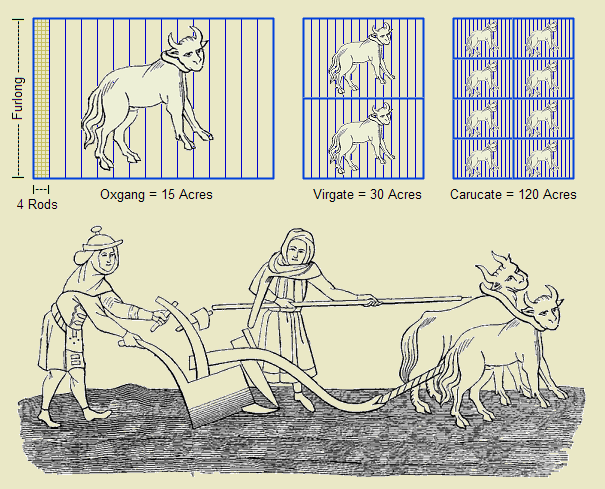
\includegraphics[max height=.45\textheight,
        max width=0.95\textwidth]{{Images/furlong}.png}
    \end{center}
    \end{column}
    \end{columns}
}
\end{frame}
\begin{frame}[t]{Round 2 --- Units of Measure --- \mbox{Answer 9}}
\vspace{-0.5em}
\begin{block}{Question}
How many feet are in a fathom? (The answer is a whole number.)
\end{block}
\visible<2->{
    \begin{block}{Answer}
    Six 
    \end{block}
}
\end{frame}
\begin{frame}[t]{Round 2 --- Units of Measure --- \mbox{Answer 10}}
\vspace{-0.5em}
\begin{block}{Question}
As of 2019, all SI (International System of Units) base units are defined in terms of fundamental physical constants and the behavior of photons and atoms. Which unit of measure was the last SI base unit to be defined by  a physical object?
\end{block}

\visible<2->{
    \begin{columns}[T,totalwidth=\linewidth]
    \begin{column}{0.7\linewidth}
    \begin{block}{Answer}
    The kilogram (which, until 2019, was defined to be the mass of a particular lump of metal stored at the International Bureau of Weights and Measures; it's now defined in terms of the meter, the second, and Planck's constant)
    \end{block}
    \end{column}
    \begin{column}{0.28\linewidth}
    \begin{center}
    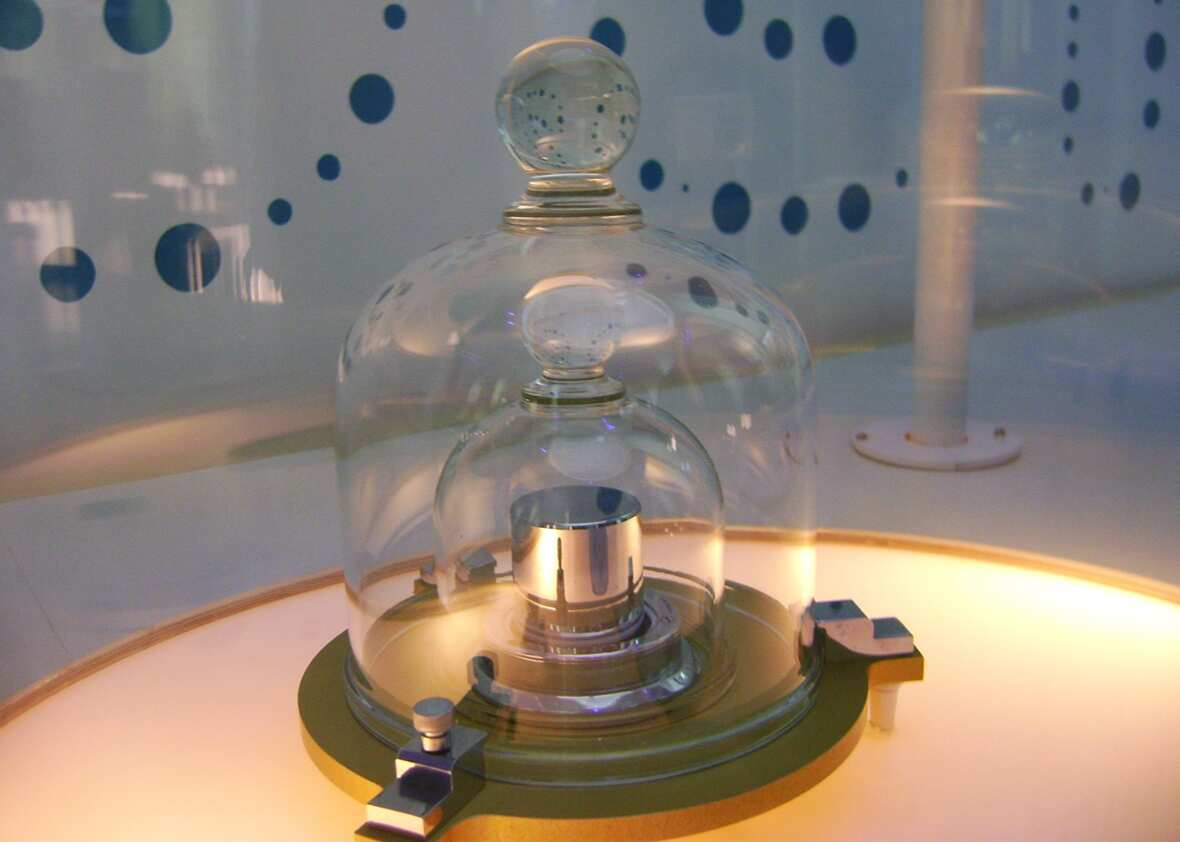
\includegraphics[max width=0.95\textwidth,
        max height=0.38000\textheight]{{Images/kilo}.jpg}
    \end{center}
    \end{column}
    \end{columns}
}
\end{frame}
\def\thisSectionName{As Seen on TV}
\section{Round 3}
\subsection*{Q1}
\begin{frame}[t]{Round 3 --- As Seen on TV --- \mbox{Question 1}}
\vspace{-0.5em}
\begin{block}{Question}
What was the first product promoted by the person who later promoted the SlapChop?
\end{block}
\end{frame}
\subsection*{Q2}
\begin{frame}[t]{Round 3 --- As Seen on TV --- \mbox{Question 2}}
\vspace{-0.5em}
\begin{block}{Question}
The name of what inventor of ``as seen on TV'' products was part of the name of his ``as seen on TV'' product company? 
\end{block}
\end{frame}
\subsection*{Q3}
\begin{frame}[t]{Round 3 --- As Seen on TV --- \mbox{Question 3}}
\vspace{-0.5em}
\begin{block}{Question}
What brand of ``as seen on TV'' tape does not come from outer space, despite its name?
\end{block}
\end{frame}
\subsection*{Q4}
\begin{frame}[t]{Round 3 --- As Seen on TV --- \mbox{Question 4}}
\vspace{-0.5em}
\begin{block}{Question}
What was the name of the fictitious product sold by Dan Aykroyd on \emph{Saturday Night Live} that could make a fish-based drink, and in just seconds? (The product was just a blender.)
\end{block}
\end{frame}
\subsection*{Q5}
\begin{frame}[t]{Round 3 --- As Seen on TV --- \mbox{Question 5}}
\vspace{-0.5em}
\begin{block}{Question}
What ``as seen on TV'' product was promoted by a boxer as a way to ``knock out the fat'' when cooking?
\end{block}
\end{frame}
\subsection*{Q6}
\begin{frame}[t]{Round 3 --- As Seen on TV --- \mbox{Question 6}}
\vspace{-0.5em}
\begin{block}{Question}
What was the first (real-life) product to be advertised in an infomercial?
\end{block}
\end{frame}
\subsection*{Q7}
\begin{frame}[t]{Round 3 --- As Seen on TV --- \mbox{Question 7}}
\vspace{-0.5em}
\begin{block}{Question}
In the ``Lucy Does a TV Commercial'' episode of \emph{I Love Lucy}, what was the name of the product that Lucy promoted?
\end{block}
\end{frame}
\subsection*{Q8}
\begin{frame}[t]{Round 3 --- As Seen on TV --- \mbox{Question 8}}
\vspace{-0.5em}
\begin{columns}[T,totalwidth=\linewidth]
\begin{column}{0.32\linewidth}
\begin{block}{Question}
What product --- a vacuum cleaner with a razor attachment to cut your hair --- is shown in the image here?
\end{block}
\end{column}
\begin{column}{0.65\linewidth}
\begin{center}
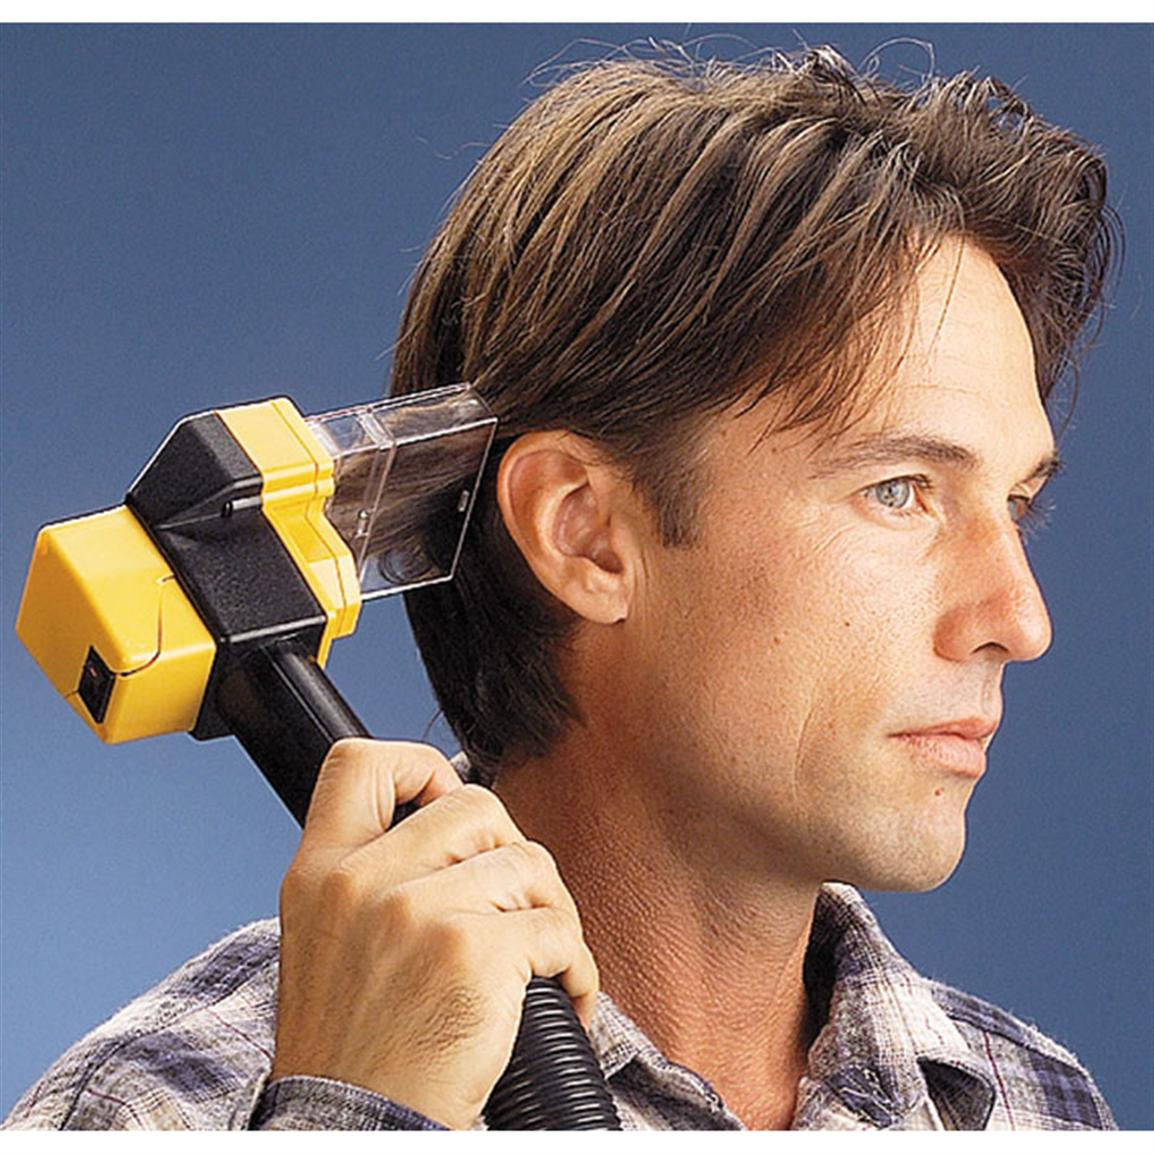
\includegraphics[max width=0.95\textwidth,max height=0.7\textheight]{{Images/flowbee}.jpeg}
\end{center}
\end{column}
\end{columns}
\end{frame}
\subsection*{Q9}
\begin{frame}[t]{Round 3 --- As Seen on TV --- \mbox{Question 9}}
\vspace{-0.5em}
\begin{block}{Question}
What ``as seen on TV'' exercise product that was designed to allow you to work on a particular part of your body was promoted by actress Suzanne Sommers?
\end{block}
\end{frame}
\subsection*{Q10}
\begin{frame}[t]{Round 3 --- As Seen on TV --- \mbox{Question 10}}
\vspace{-0.5em}
\begin{columns}[T,totalwidth=\linewidth]
\begin{column}{0.32\linewidth}
\begin{block}{Question}
Pictured here are the pallbearers for which person's funeral?
\end{block}
\end{column}
\begin{column}{0.65\linewidth}
\begin{center}
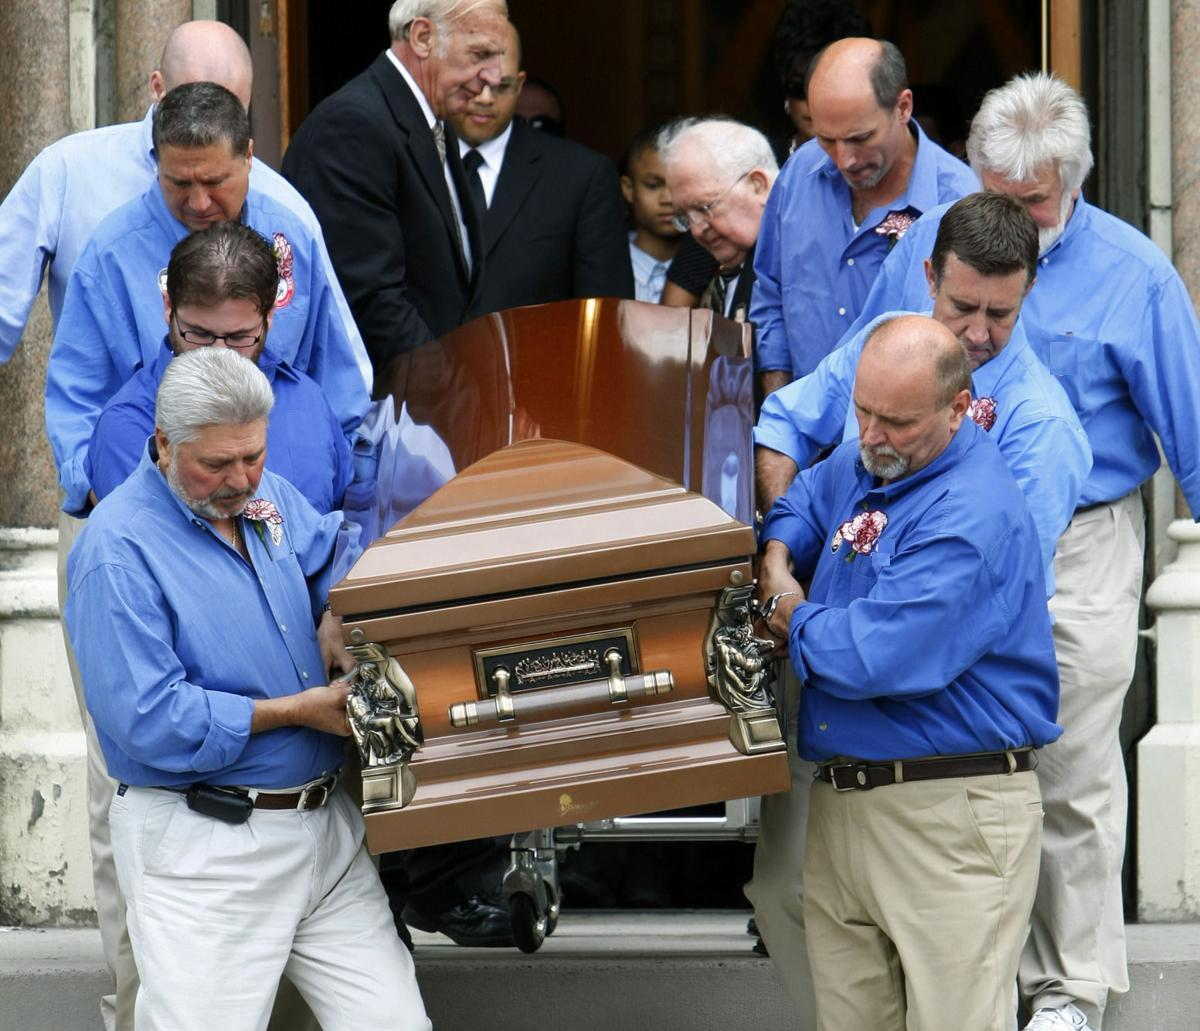
\includegraphics[max width=0.95\textwidth,max height=0.7\textheight]{{Images/billymays}.jpg}
\end{center}
\end{column}
\end{columns}
\end{frame}
\subsection{Answers}
\begin{frame}[t]{Round 3 --- As Seen on TV --- \mbox{Answer 1}}
\vspace{-0.5em}
\begin{block}{Question}
What was the first product promoted by the person who later promoted the SlapChop?
\end{block}

\visible<2->{
    \begin{columns}[T,totalwidth=\linewidth]
    \begin{column}{0.32\linewidth}
    \begin{block}{Answer}
    The ShamWow (Vince Shlomi)
    \end{block}
    \end{column}
    \begin{column}{0.65\linewidth}
    \begin{center}
    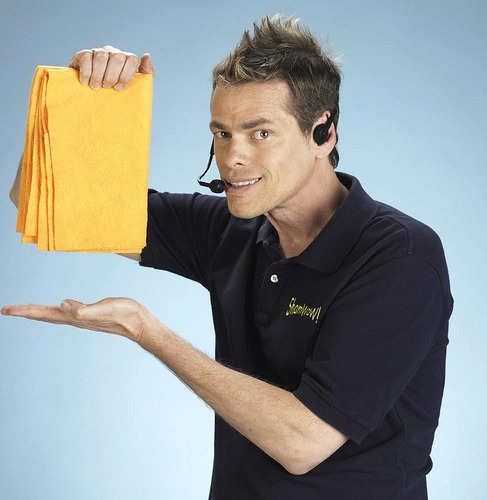
\includegraphics[max height=.45\textheight,
        max width=0.95\textwidth]{{Images/shamwow}.jpg}
    \end{center}
    \end{column}
    \end{columns}
}
\end{frame}
\begin{frame}[t]{Round 3 --- As Seen on TV --- \mbox{Answer 2}}
\vspace{-0.5em}
\begin{block}{Question}
The name of what inventor of ``as seen on TV'' products was part of the name of his ``as seen on TV'' product company? 
\end{block}

\visible<2->{
    \begin{columns}[T,totalwidth=\linewidth]
    \begin{column}{0.32\linewidth}
    \begin{block}{Answer}
    Ron Popeil (the company was Ronco)
    \end{block}
    \end{column}
    \begin{column}{0.65\linewidth}
    \begin{center}
    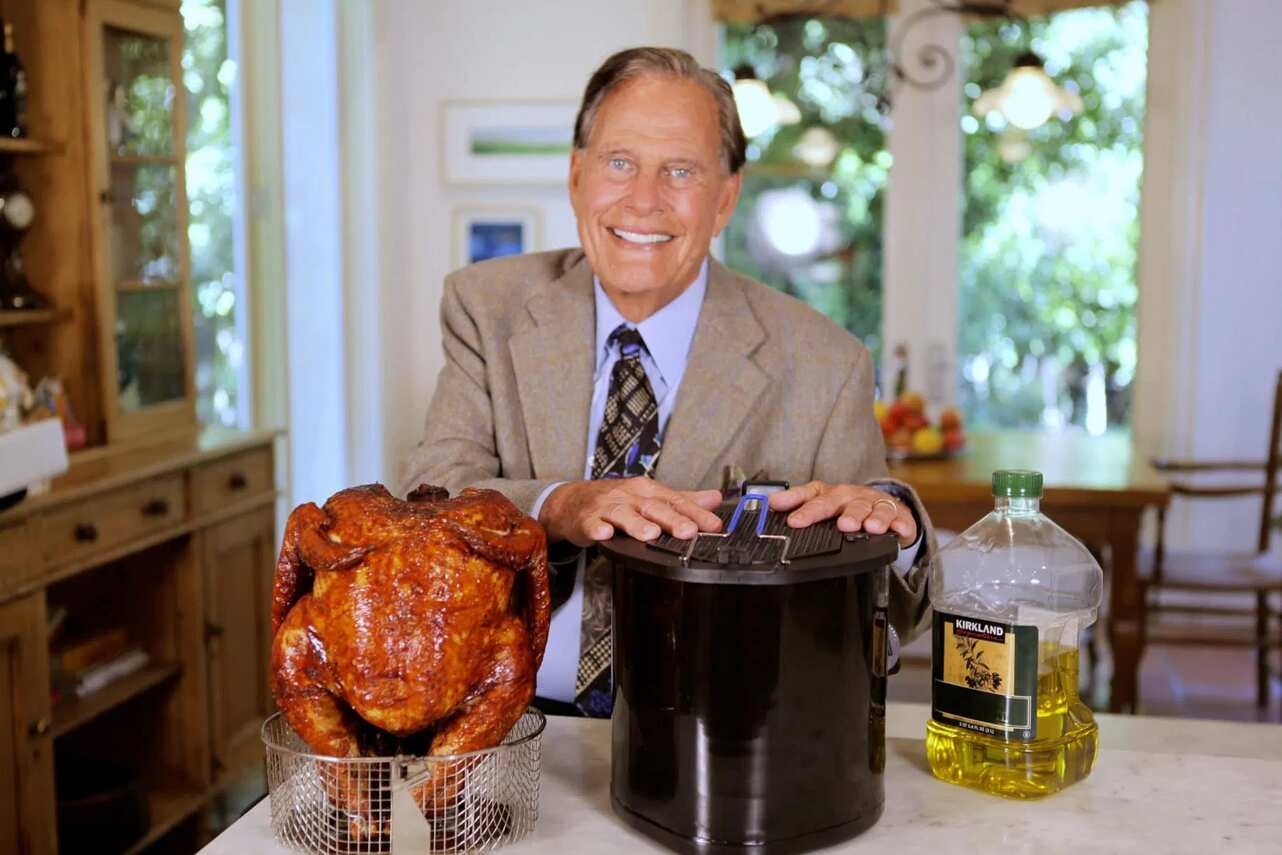
\includegraphics[max height=.45\textheight,
        max width=0.95\textwidth]{{Images/ronco}.jpg}
    \end{center}
    \end{column}
    \end{columns}
}
\end{frame}
\begin{frame}[t]{Round 3 --- As Seen on TV --- \mbox{Answer 3}}
\vspace{-0.5em}
\begin{block}{Question}
What brand of ``as seen on TV'' tape does not come from outer space, despite its name?
\end{block}

\visible<2->{
    \begin{columns}[T,totalwidth=\linewidth]
    \begin{column}{0.32\linewidth}
    \begin{block}{Answer}
    Alien Tape
    \end{block}
    \end{column}
    \begin{column}{0.65\linewidth}
    \begin{center}
    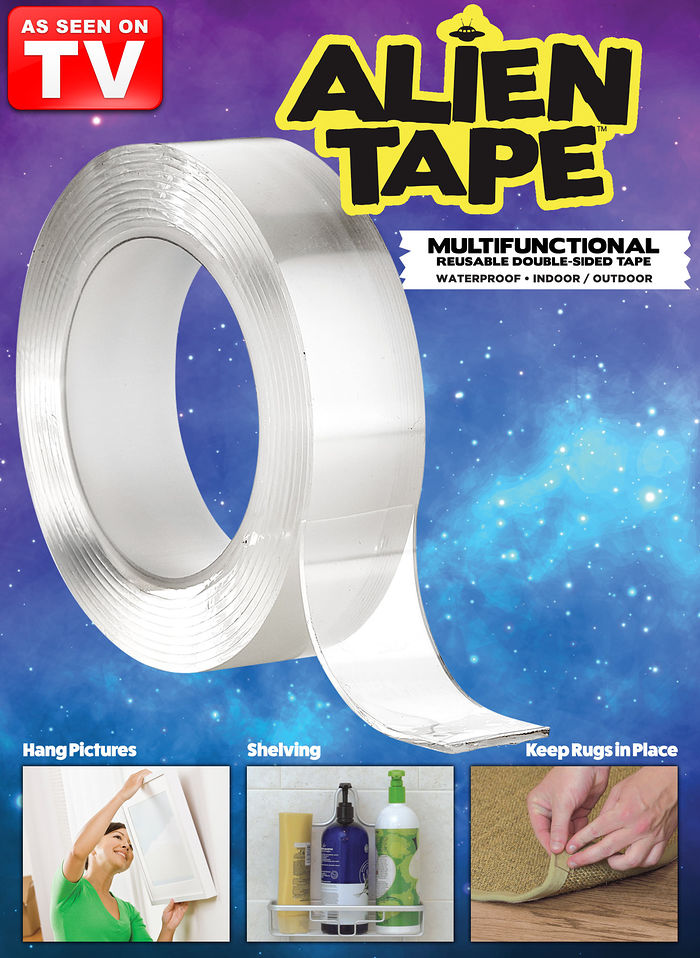
\includegraphics[max height=.45\textheight,
        max width=0.95\textwidth]{{Images/alientape}.jpg}
    \end{center}
    \end{column}
    \end{columns}
}
\end{frame}
\begin{frame}[t]{Round 3 --- As Seen on TV --- \mbox{Answer 4}}
\vspace{-0.5em}
\begin{block}{Question}
What was the name of the fictitious product sold by Dan Aykroyd on \emph{Saturday Night Live} that could make a fish-based drink, and in just seconds? (The product was just a blender.)
\end{block}

\visible<2->{
    \begin{columns}[T,totalwidth=\linewidth]
    \begin{column}{0.32\linewidth}
    \begin{block}{Answer}
    The Bass-o-Matic
    \end{block}
    \end{column}
    \begin{column}{0.65\linewidth}
    \begin{center}
    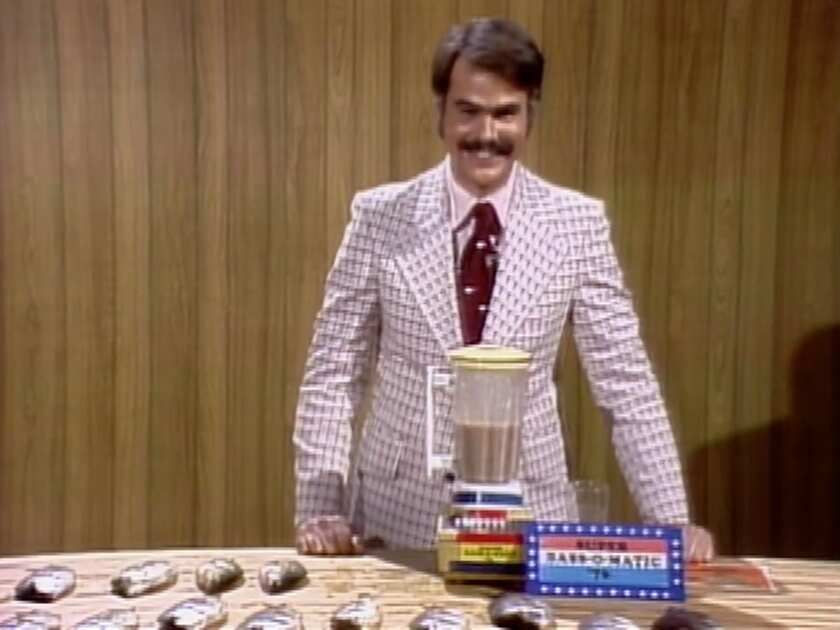
\includegraphics[max height=.45\textheight,
        max width=0.95\textwidth]{{Images/bassomatic}.jpg}
    \end{center}
    \end{column}
    \end{columns}
}
\end{frame}
\begin{frame}[t]{Round 3 --- As Seen on TV --- \mbox{Answer 5}}
\vspace{-0.5em}
\begin{block}{Question}
What ``as seen on TV'' product was promoted by a boxer as a way to ``knock out the fat'' when cooking?
\end{block}

\visible<2->{
    \begin{columns}[T,totalwidth=\linewidth]
    \begin{column}{0.32\linewidth}
    \begin{block}{Answer}
    The George Foreman Lean Mean Fat-Reducing Grilling Machine / George Foreman Grill
    \end{block}
    \end{column}
    \begin{column}{0.65\linewidth}
    \begin{center}
    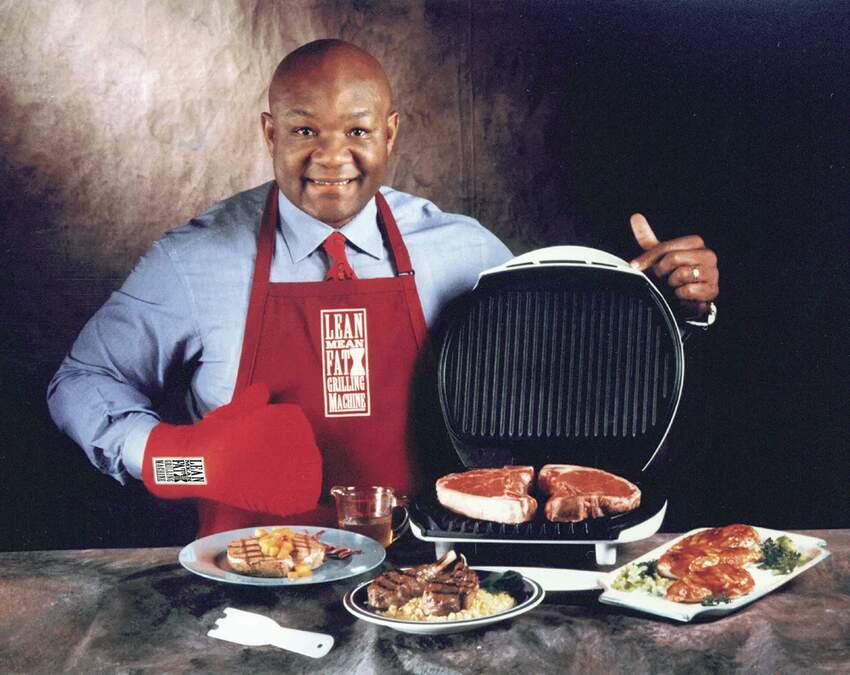
\includegraphics[max height=.45\textheight,
        max width=0.95\textwidth]{{Images/foreman}.jpg}
    \end{center}
    \end{column}
    \end{columns}
}
\end{frame}
\begin{frame}[t]{Round 3 --- As Seen on TV --- \mbox{Answer 6}}
\vspace{-0.5em}
\begin{block}{Question}
What was the first (real-life) product to be advertised in an infomercial?
\end{block}

\visible<2->{
    \begin{columns}[T,totalwidth=\linewidth]
    \begin{column}{0.32\linewidth}
    \begin{block}{Answer}
    The Vitamix blender (1950)
    \end{block}
    \end{column}
    \begin{column}{0.65\linewidth}
    \begin{center}
    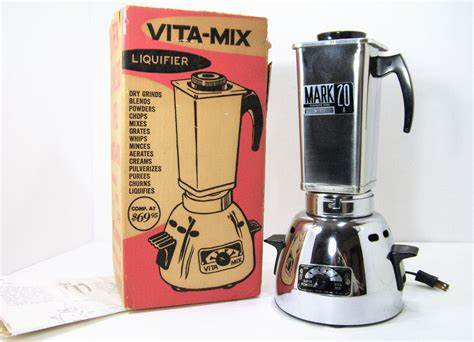
\includegraphics[max height=.45\textheight,
        max width=0.95\textwidth]{{Images/vitamix}.jpeg}
    \end{center}
    \end{column}
    \end{columns}
}
\end{frame}
\begin{frame}[t]{Round 3 --- As Seen on TV --- \mbox{Answer 7}}
\vspace{-0.5em}
\begin{block}{Question}
In the ``Lucy Does a TV Commercial'' episode of \emph{I Love Lucy}, what was the name of the product that Lucy promoted?
\end{block}

\visible<2->{
    \begin{columns}[T,totalwidth=\linewidth]
    \begin{column}{0.32\linewidth}
    \begin{block}{Answer}
    Vitameatavegamin (we'll be flexible on the vowels, but you do have to have all the right consonants in the right order)
    \end{block}
    \end{column}
    \begin{column}{0.65\linewidth}
    \begin{center}
    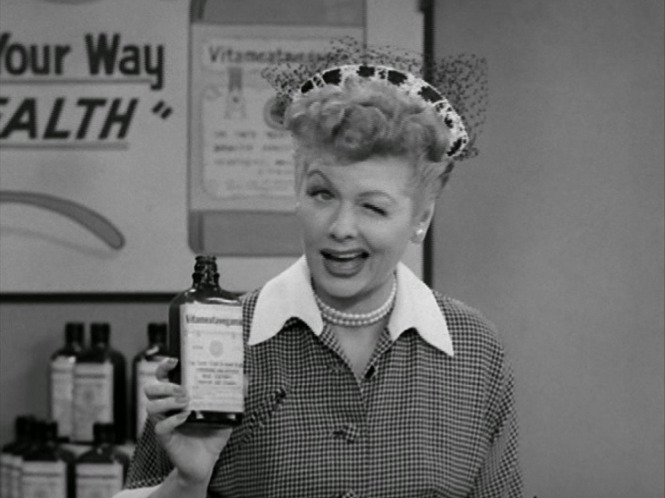
\includegraphics[max height=.45\textheight,
        max width=0.95\textwidth]{{Images/lucy}.jpg}
    \end{center}
    \end{column}
    \end{columns}
}
\end{frame}
\begin{frame}[t]{Round 3 --- As Seen on TV --- \mbox{Answer 8}}
\vspace{-0.5em}
\begin{columns}[T,totalwidth=\linewidth]
\begin{column}{0.32\linewidth}
\begin{block}{Question}
What product --- a vacuum cleaner with a razor attachment to cut your hair --- is shown in the image here?
\end{block}
\visible<2->{
    \begin{block}{Answer}
    The Flowbee
    \end{block}
}
\end{column}
\begin{column}{0.65\linewidth}
\begin{center}
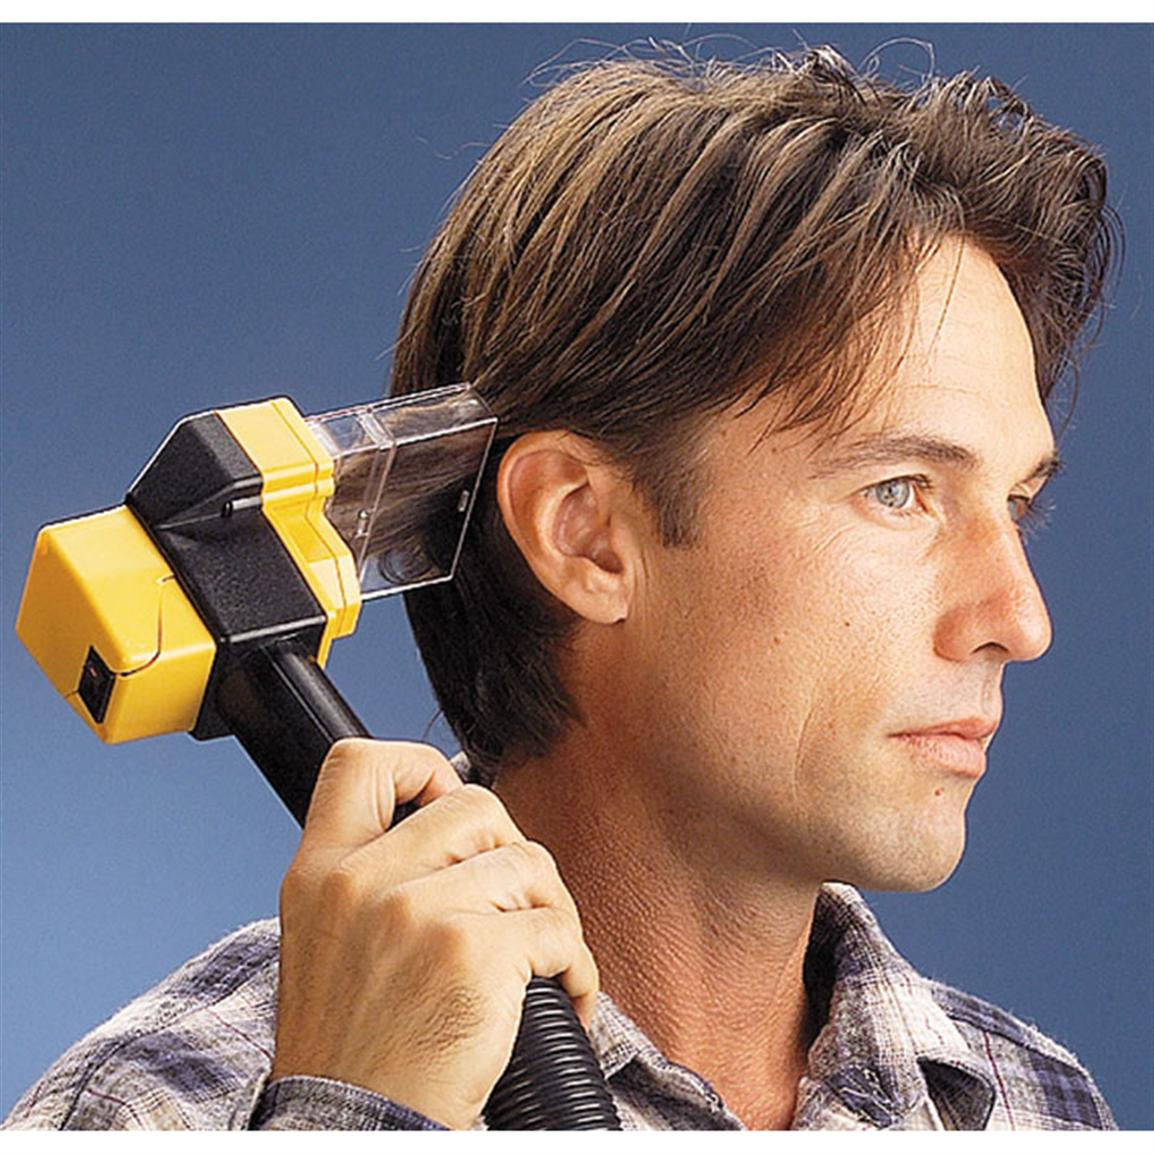
\includegraphics[max width=0.95\textwidth,max height=0.7\textheight]{{Images/flowbee}.jpeg}
\end{center}
\end{column}
\end{columns}
\end{frame}
\begin{frame}[t]{Round 3 --- As Seen on TV --- \mbox{Answer 9}}
\vspace{-0.5em}
\begin{block}{Question}
What ``as seen on TV'' exercise product that was designed to allow you to work on a particular part of your body was promoted by actress Suzanne Sommers?
\end{block}

\visible<2->{
    \begin{columns}[T,totalwidth=\linewidth]
    \begin{column}{0.32\linewidth}
    \begin{block}{Answer}
    The Thighmaster
    \end{block}
    \end{column}
    \begin{column}{0.65\linewidth}
    \begin{center}
    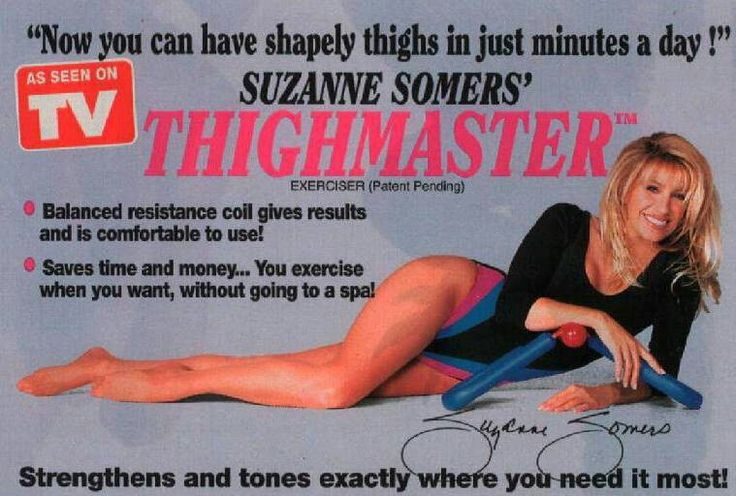
\includegraphics[max height=.45\textheight,
        max width=0.95\textwidth]{{Images/thighmaster}.jpg}
    \end{center}
    \end{column}
    \end{columns}
}
\end{frame}
\begin{frame}[t]{Round 3 --- As Seen on TV --- \mbox{Answer 10}}
\vspace{-0.5em}
\begin{columns}[T,totalwidth=\linewidth]
\begin{column}{0.38\linewidth}
\begin{block}{Question}
Pictured here are the pallbearers for which person's funeral?
\end{block}
\end{column}
\begin{column}{0.6\linewidth}
\begin{center}
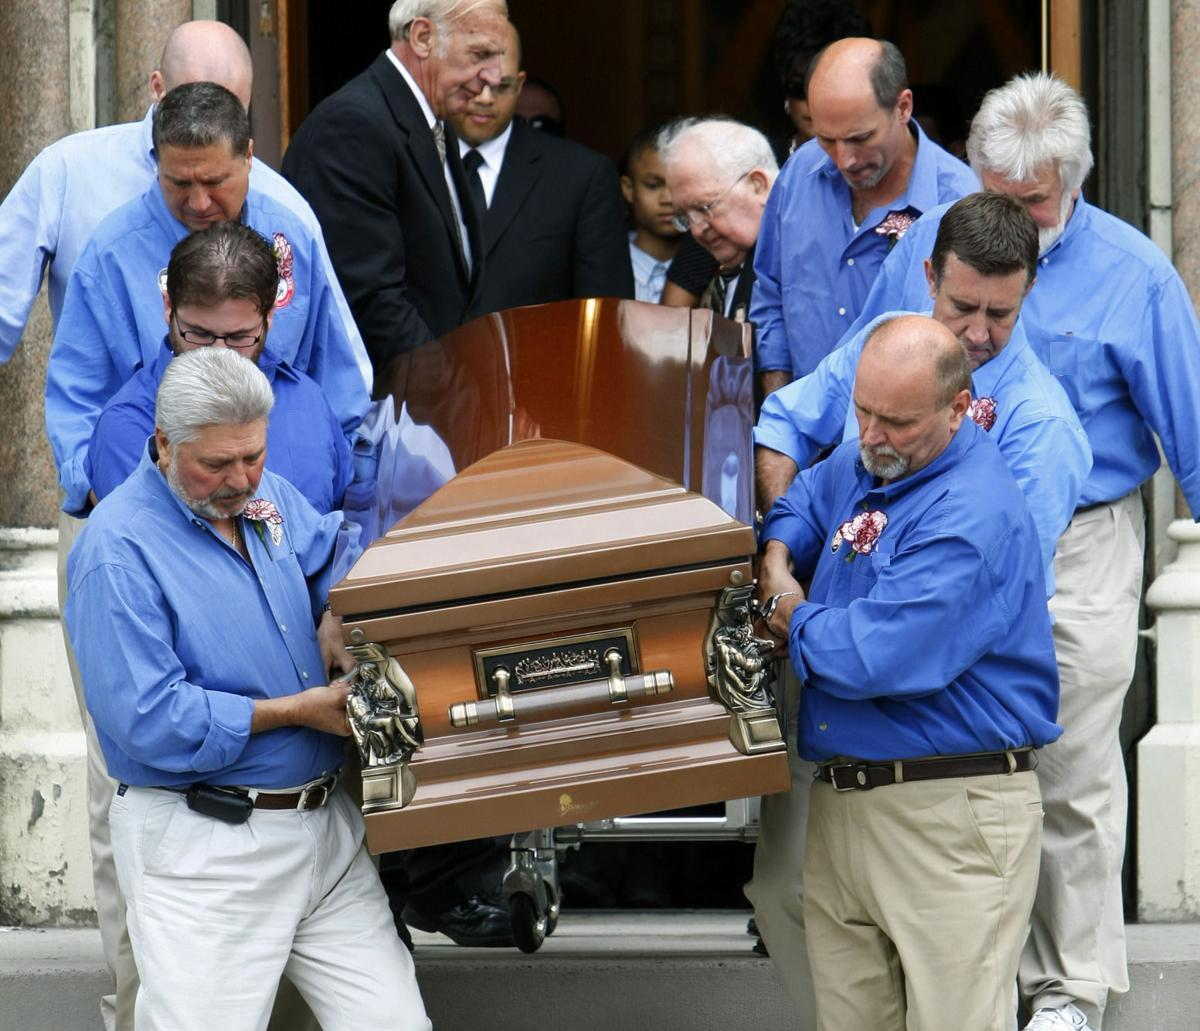
\includegraphics[max width=0.95\textwidth,max height=0.35\textheight]{{Images/billymays}.jpg}
\end{center}
\end{column}
\end{columns}

\visible<2->{
    \begin{columns}[T,totalwidth=\linewidth]
    \begin{column}{0.38\linewidth}
    \begin{block}{Answer}
    Billy Mays
    \end{block}
    \end{column}
    \begin{column}{0.6\linewidth}
    \begin{center}
    
\includegraphics[max width=0.95\textwidth,
        max height=0.34\textheight]{{Images/billymaysperson}.jpg}
    \end{center}
    \end{column}
    \end{columns}
}
\end{frame}
\def\thisSectionName{Spring}
\section{Round 4}
\subsection*{Q1}
\begin{frame}[t]{Round 4 --- Spring --- \mbox{Question 1}}
\vspace{-0.5em}
\begin{block}{Question}
Which song from Rodgers and Hammerstein's musical film \emph{State Fair} has the word ``spring'' in the title? 
\end{block}
\end{frame}
\subsection*{Q2}
\begin{frame}[t]{Round 4 --- Spring --- \mbox{Question 2}}
\vspace{-0.5em}
\begin{block}{Question}
In Major League Baseball's spring training season, the teams collectively known as the ``Cactus League'' hold spring training in which U.S. state?
\end{block}
\end{frame}
\subsection*{Q3}
\begin{frame}[t]{Round 4 --- Spring --- \mbox{Question 3}}
\vspace{-0.5em}
\begin{block}{Question}
What DC Comics character shares a name with a harbinger of spring?
\end{block}
\end{frame}
\subsection*{Q4}
\begin{frame}[t]{Round 4 --- Spring --- \mbox{Question 4}}
\vspace{-0.5em}
\begin{block}{Question}
Who composed the music for the 1913 ballet \emph{The Rite of Spring}?
\end{block}
\end{frame}
\subsection*{Q5}
\begin{frame}[t]{Round 4 --- Spring --- \mbox{Question 5}}
\vspace{-0.5em}
\begin{block}{Question}
Until recent years, what type of birds returned in large numbers to California's Mission San Juan Capistrano annually in March?
\end{block}
\end{frame}
\subsection*{Q6}
\begin{frame}[t]{Round 4 --- Spring --- \mbox{Question 6}}
\vspace{-0.5em}
\begin{block}{Question}
Complete the line of the first line of this poem, which has been called ``The Brooklyn National Anthem'': ``Spring has sprung, \textunderscore{}\textunderscore{}\textunderscore{}\textunderscore{}\textunderscore{} \textunderscore{}\textunderscore{}\textunderscore{}\textunderscore{}\textunderscore{} \textunderscore{}\textunderscore{}\textunderscore{}\textunderscore{}\textunderscore{} \textunderscore{}\textunderscore{}\textunderscore{}\textunderscore{}\textunderscore{}'' (four words)
\end{block}
\end{frame}
\subsection*{Q7}
\begin{frame}[t]{Round 4 --- Spring --- \mbox{Question 7}}
\vspace{-0.5em}
\begin{block}{Question}
Which spring commemorative day, first observed in 1872, is dedicated to the planting of trees?
\end{block}
\end{frame}
\subsection*{Q8}
\begin{frame}[t]{Round 4 --- Spring --- \mbox{Question 8}}
\vspace{-0.5em}
\begin{block}{Question}
Which spring-flowering plant was named after  William Forsyth (1737--1804), a Scottish botanist who was the head royal gardener?
\end{block}
\end{frame}
\subsection*{Q9}
\begin{frame}[t]{Round 4 --- Spring --- \mbox{Question 9}}
\vspace{-0.5em}
\begin{block}{Question}
What famous literary work situated its narrative in springtime with the following opening lines:
\begin{quotation}
Whan that aprill with his shoures soote\\
The droghte of march hath perced to the roote,\\
And bathed every veyne in swich licour\\
Of which vertu engendred is the flour\ldots
\end{quotation}
\end{block}
\end{frame}
\subsection*{Q10}
\begin{frame}[t]{Round 4 --- Spring --- \mbox{Question 10}}
\vspace{-0.5em}
\begin{block}{Question}
This year, what is the date of the vernal equinox in the Northern Hemisphere?
\end{block}
\end{frame}
\subsection{Answers}
\begin{frame}[t]{Round 4 --- Spring --- \mbox{Answer 1}}
\vspace{-0.5em}
\begin{block}{Question}
Which song from Rodgers and Hammerstein's musical film \emph{State Fair} has the word ``spring'' in the title? 
\end{block}

\visible<2->{
    \begin{columns}[T,totalwidth=\linewidth]
    \begin{column}{0.32\linewidth}
    \begin{block}{Answer}
    ``It Might as Well be Spring''
    \end{block}
    \end{column}
    \begin{column}{0.65\linewidth}
    \begin{center}
    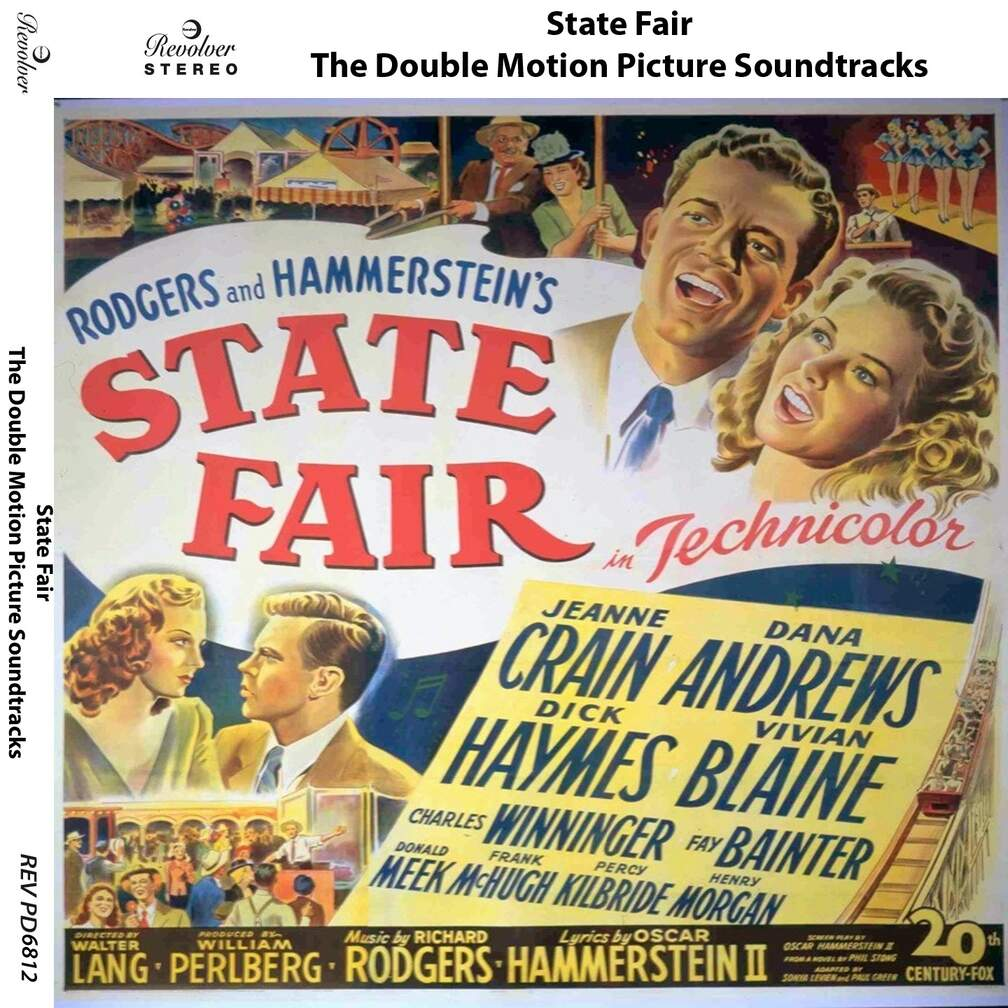
\includegraphics[max height=.45\textheight,
        max width=0.95\textwidth]{{Images/hammerstein}.jpg}
    \end{center}
    \end{column}
    \end{columns}
}
\end{frame}
\begin{frame}[t]{Round 4 --- Spring --- \mbox{Answer 2}}
\vspace{-0.5em}
\begin{block}{Question}
In Major League Baseball's spring training season, the teams collectively known as the ``Cactus League'' hold spring training in which U.S. state?
\end{block}

\visible<2->{
    \begin{columns}[T,totalwidth=\linewidth]
    \begin{column}{0.32\linewidth}
    \begin{block}{Answer}
    Arizona
    \end{block}
    \end{column}
    \begin{column}{0.65\linewidth}
    \begin{center}
    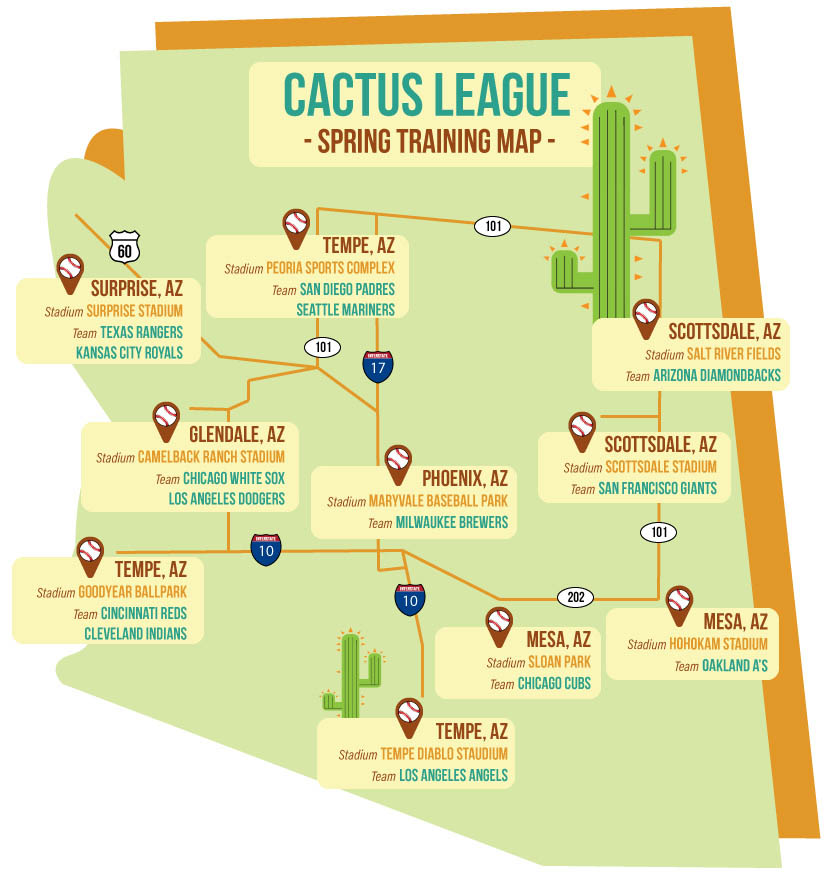
\includegraphics[max height=.45\textheight,
        max width=0.95\textwidth]{{Images/cactus}.jpg}
    \end{center}
    \end{column}
    \end{columns}
}
\end{frame}
\begin{frame}[t]{Round 4 --- Spring --- \mbox{Answer 3}}
\vspace{-0.5em}
\begin{block}{Question}
What DC Comics character shares a name with a harbinger of spring?
\end{block}

\visible<2->{
    \begin{columns}[T,totalwidth=\linewidth]
    \begin{column}{0.32\linewidth}
    \begin{block}{Answer}
    Robin
    \end{block}
    \end{column}
    \begin{column}{0.65\linewidth}
    \begin{center}
    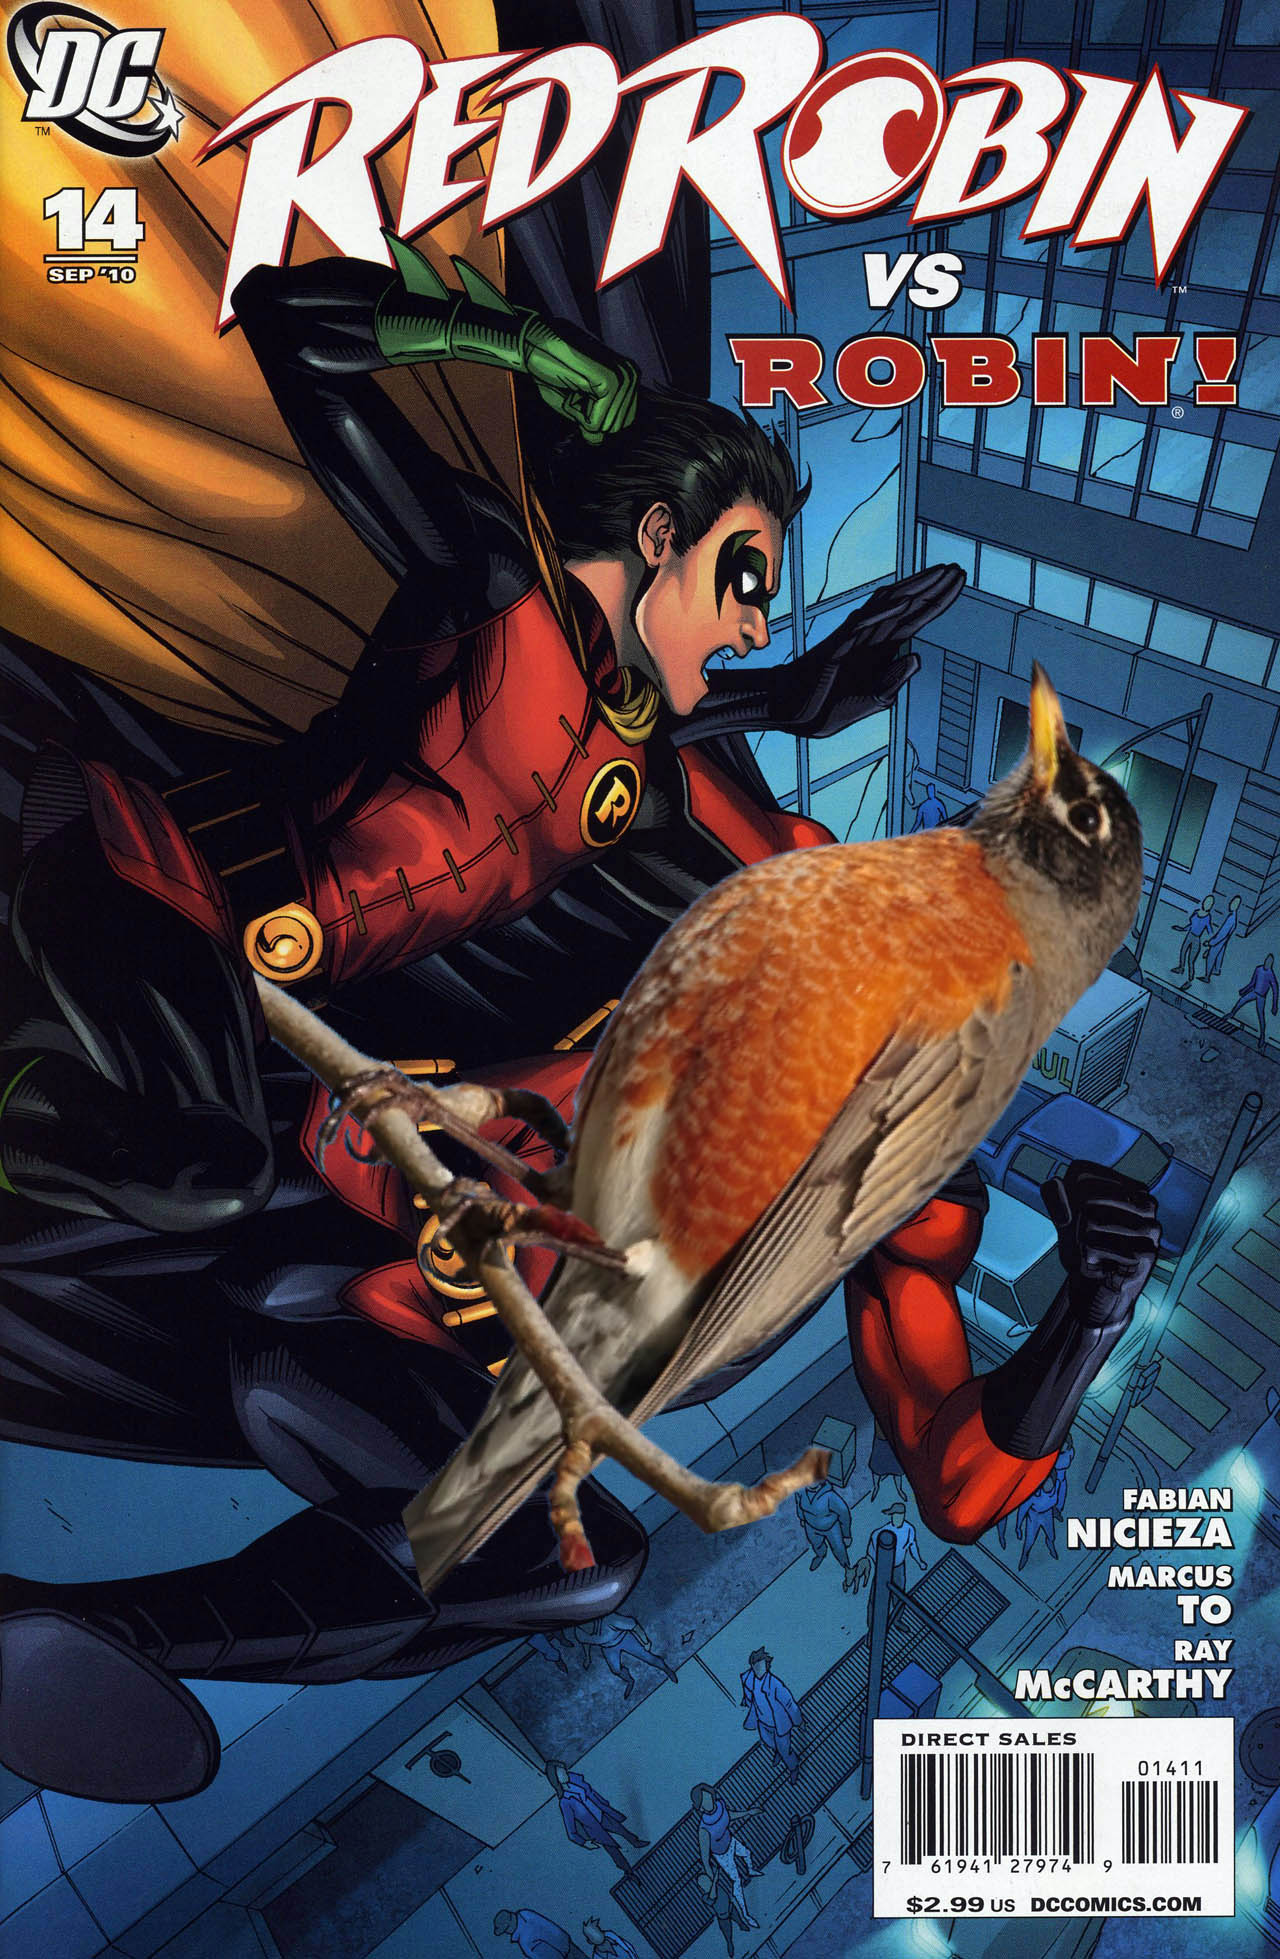
\includegraphics[max height=.45\textheight,
        max width=0.95\textwidth]{{Images/robin}.jpg}
    \end{center}
    \end{column}
    \end{columns}
}
\end{frame}
\begin{frame}[t]{Round 4 --- Spring --- \mbox{Answer 4}}
\vspace{-0.5em}
\begin{block}{Question}
Who composed the music for the 1913 ballet \emph{The Rite of Spring}?
\end{block}

\visible<2->{
    \begin{columns}[T,totalwidth=\linewidth]
    \begin{column}{0.32\linewidth}
    \begin{block}{Answer}
    Igor Stravinsky
    \end{block}
    \end{column}
    \begin{column}{0.65\linewidth}
    \begin{center}
    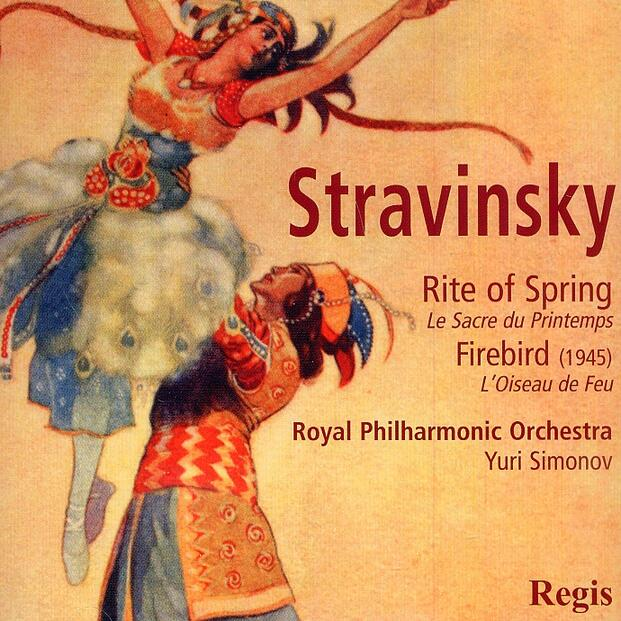
\includegraphics[max height=.45\textheight,
        max width=0.95\textwidth]{{Images/stravinsky}.jpg}
    \end{center}
    \end{column}
    \end{columns}
}
\end{frame}
\begin{frame}[t]{Round 4 --- Spring --- \mbox{Answer 5}}
\vspace{-0.5em}
\begin{block}{Question}
Until recent years, what type of birds returned in large numbers to California's Mission San Juan Capistrano annually in March?
\end{block}

\visible<2->{
    \begin{columns}[T,totalwidth=\linewidth]
    \begin{column}{0.32\linewidth}
    \begin{block}{Answer}
    Swallows
    \end{block}
    \end{column}
    \begin{column}{0.65\linewidth}
    \begin{center}
    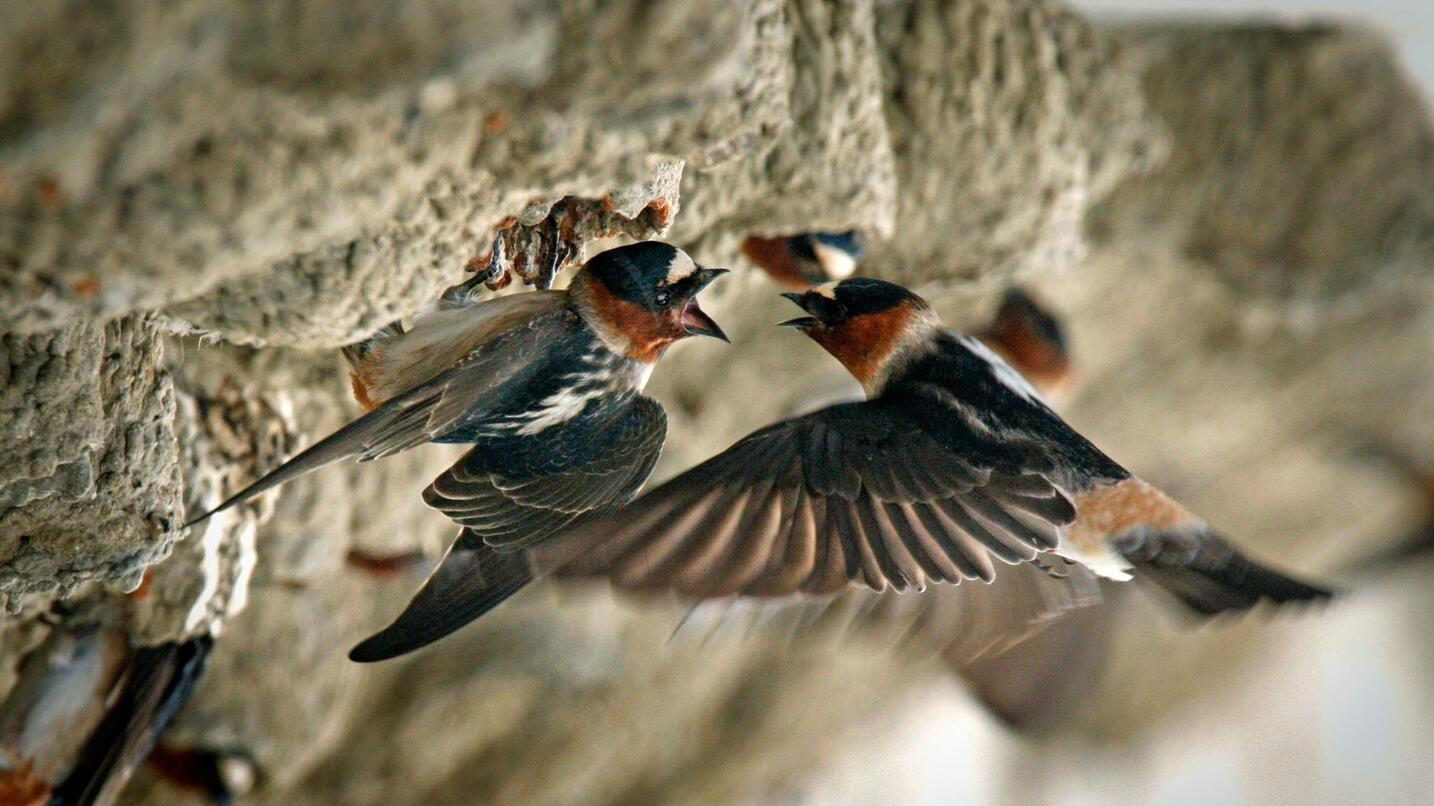
\includegraphics[max height=.45\textheight,
        max width=0.95\textwidth]{{Images/swallows}.jpg}
    \end{center}
    \end{column}
    \end{columns}
}
\end{frame}
\begin{frame}[t]{Round 4 --- Spring --- \mbox{Answer 6}}
\vspace{-0.5em}
\begin{block}{Question}
Complete the line of the first line of this poem, which has been called ``The Brooklyn National Anthem'': ``Spring has sprung, \textunderscore{}\textunderscore{}\textunderscore{}\textunderscore{}\textunderscore{} \textunderscore{}\textunderscore{}\textunderscore{}\textunderscore{}\textunderscore{} \textunderscore{}\textunderscore{}\textunderscore{}\textunderscore{}\textunderscore{} \textunderscore{}\textunderscore{}\textunderscore{}\textunderscore{}\textunderscore{}'' (four words)
\end{block}
\visible<2->{
    \begin{block}{Answer}
    The grass is ris (spelling not important, but the vowel in ``ris'' is a short I). Here is the full poem:
\begin{verse}
Spring has sprung, the grass is ris,\\ 
I wonder where the boidies is \\
The boid is on the wing, \\
But that's absoid \\
From what I hoid \\
The wing is on the boid!
\end{verse}
    \end{block}
}
\end{frame}
\begin{frame}[t]{Round 4 --- Spring --- \mbox{Answer 7}}
\vspace{-0.5em}
\begin{block}{Question}
Which spring commemorative day, first observed in 1872, is dedicated to the planting of trees?
\end{block}

\visible<2->{
    \begin{columns}[T,totalwidth=\linewidth]
    \begin{column}{0.32\linewidth}
    \begin{block}{Answer}
    Arbor Day
    \end{block}
    \end{column}
    \begin{column}{0.65\linewidth}
    \begin{center}
    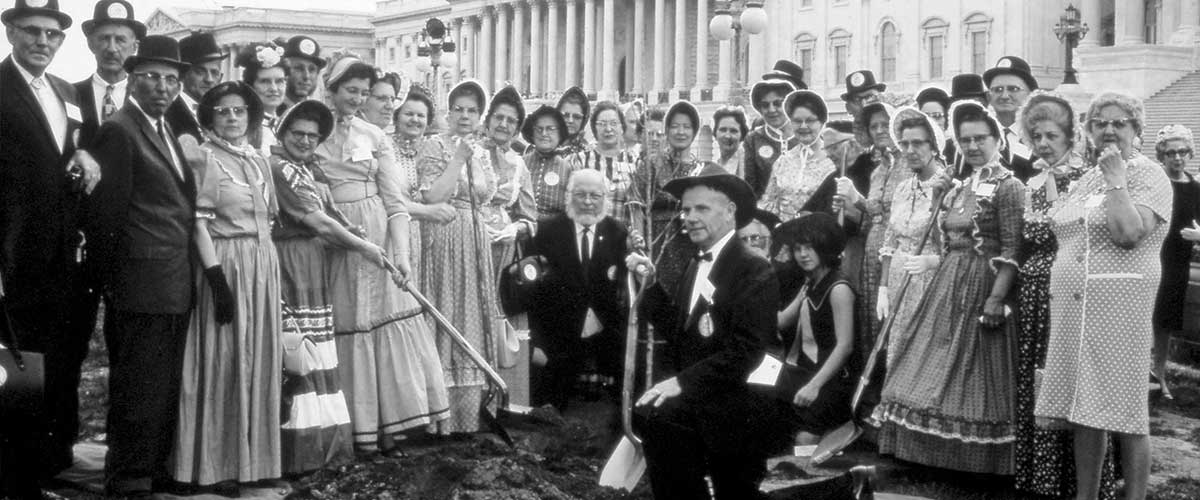
\includegraphics[max height=.45\textheight,
        max width=0.95\textwidth]{{Images/arborday}.jpg}
    \end{center}
    \end{column}
    \end{columns}
}
\end{frame}
\begin{frame}[t]{Round 4 --- Spring --- \mbox{Answer 8}}
\vspace{-0.5em}
\begin{block}{Question}
Which spring-flowering plant was named after  William Forsyth (1737--1804), a Scottish botanist who was the head royal gardener?
\end{block}

\visible<2->{
    \begin{columns}[T,totalwidth=\linewidth]
    \begin{column}{0.32\linewidth}
    \begin{block}{Answer}
    Forsythia 
    \end{block}
    \end{column}
    \begin{column}{0.65\linewidth}
    \begin{center}
    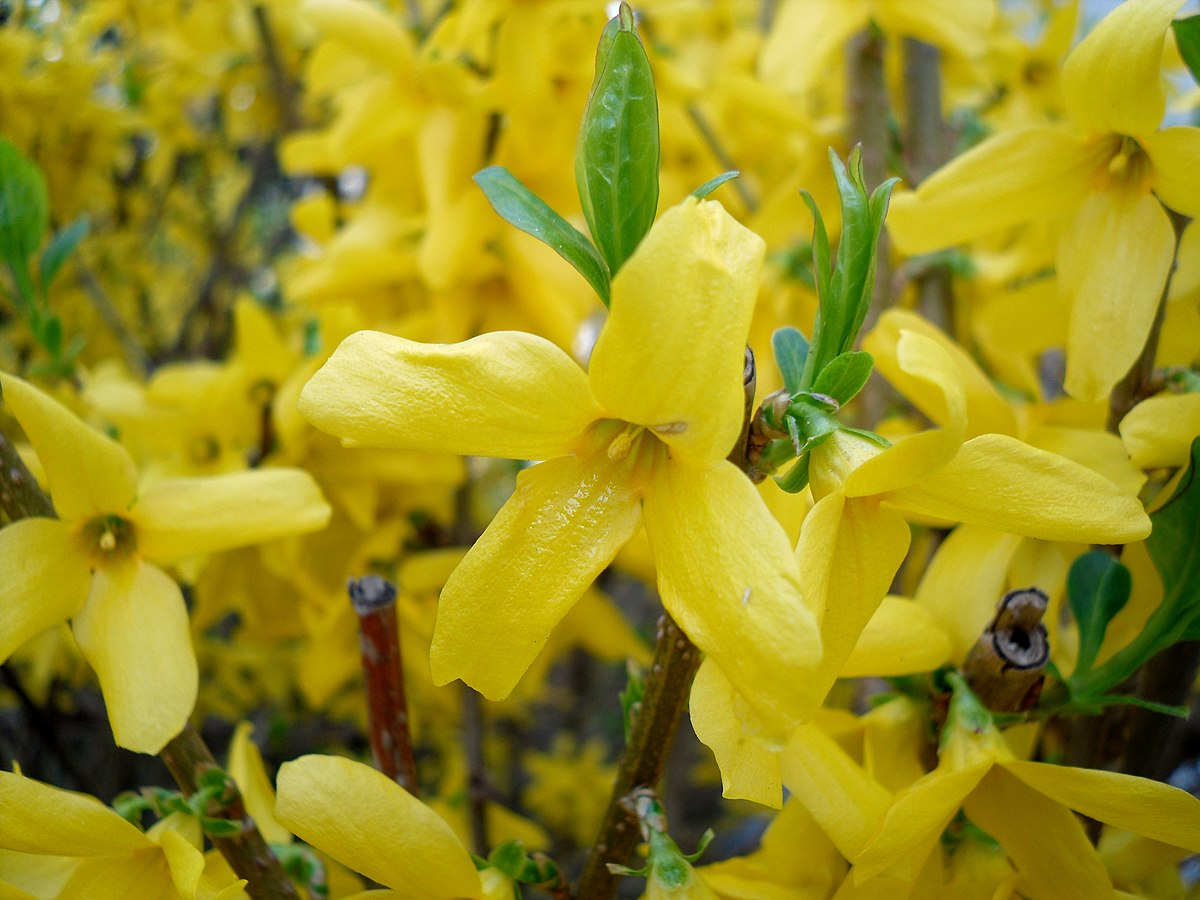
\includegraphics[max height=.45\textheight,
        max width=0.95\textwidth]{{Images/forsythia}.JPG}
    \end{center}
    \end{column}
    \end{columns}
}
\end{frame}
\begin{frame}[t]{Round 4 --- Spring --- \mbox{Answer 9}}
\vspace{-0.5em}
\begin{block}{Question}
What famous literary work situated its narrative in springtime with the following opening lines:
\begin{quotation}
Whan that aprill with his shoures soote\\
The droghte of march hath perced to the roote,\\
And bathed every veyne in swich licour\\
Of which vertu engendred is the flour\ldots
\end{quotation}
\end{block}

\visible<2->{
    \begin{columns}[T,totalwidth=\linewidth]
    \begin{column}{0.32\linewidth}
    \begin{block}{Answer}
    \emph{The Canterbury Tales}
    \end{block}
    \end{column}
    \begin{column}{0.65\linewidth}
    \begin{center}
    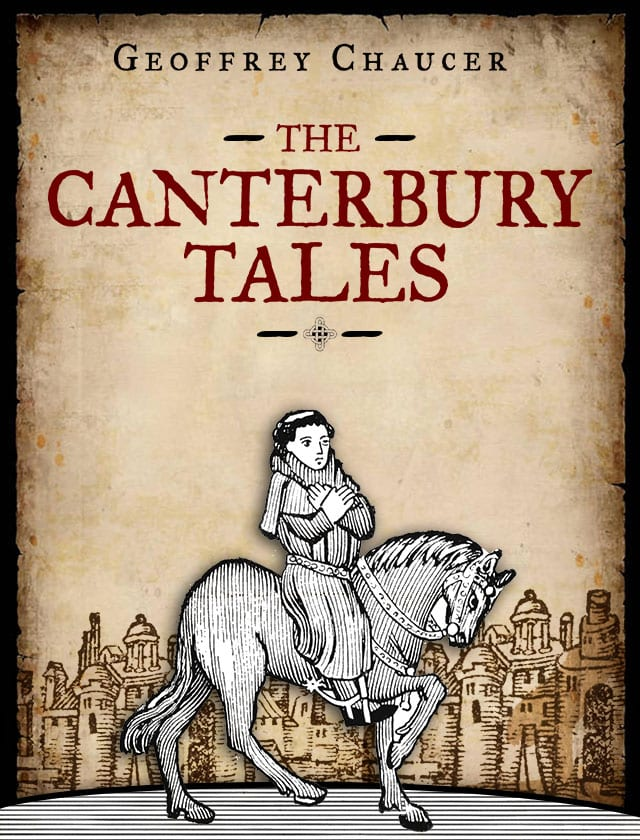
\includegraphics[max height=.45\textheight,
        max width=0.95\textwidth]{{Images/canterbury}.jpg}
    \end{center}
    \end{column}
    \end{columns}
}
\end{frame}
\begin{frame}[t]{Round 4 --- Spring --- \mbox{Answer 10}}
\vspace{-0.5em}
\begin{block}{Question}
This year, what is the date of the vernal equinox in the Northern Hemisphere?
\end{block}

\visible<2->{
    \begin{columns}[T,totalwidth=\linewidth]
    \begin{column}{0.32\linewidth}
    \begin{block}{Answer}
    Today! (March 20)
    \end{block}
    \end{column}
    \begin{column}{0.65\linewidth}
    \begin{center}
    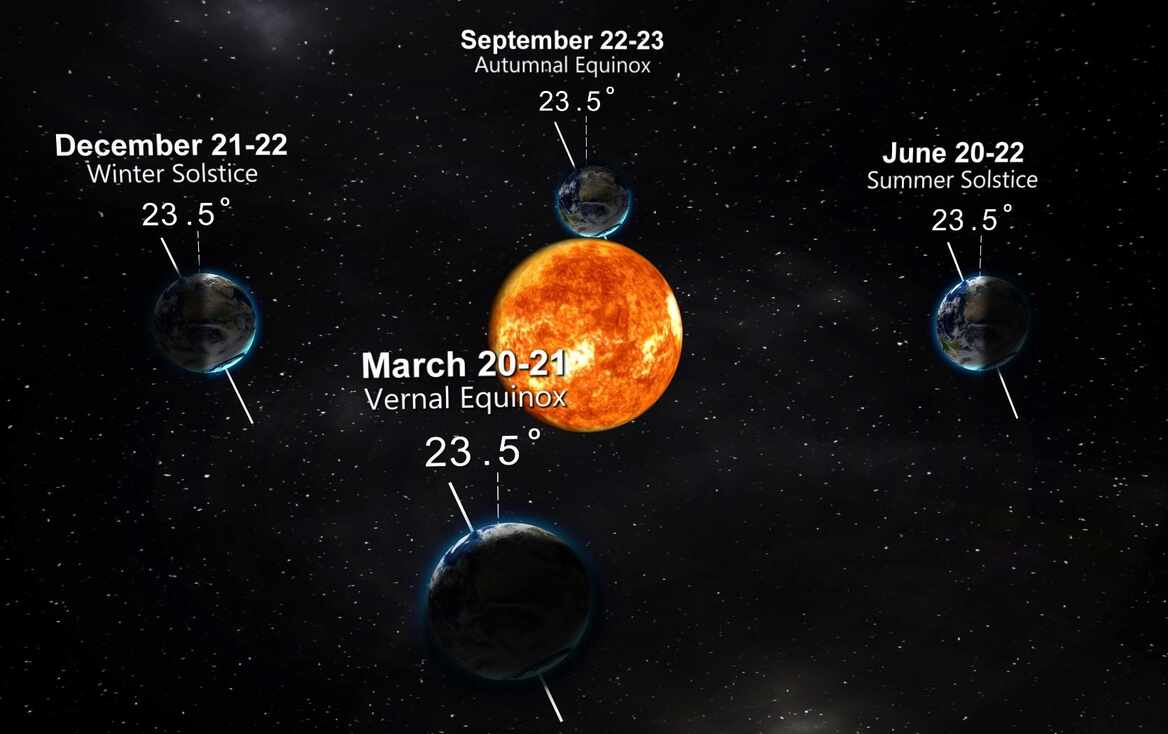
\includegraphics[max height=.45\textheight,
        max width=0.95\textwidth]{{Images/vernalequinox}.jpg}
    \end{center}
    \end{column}
    \end{columns}
}
\end{frame}
\def\thisSectionName{Portmanteaus}
\section{Round 5}
\subsection*{Q1}
\begin{frame}[t]{Round 5 --- Portmanteaus --- \mbox{Question 1}}
\vspace{-0.5em}
\begin{block}{Question}
What is the name of the annual month-long event during which men grow facial hair in order to raise awareness around men's health issues?
\end{block}
\end{frame}
\subsection*{Q2}
\begin{frame}[t]{Round 5 --- Portmanteaus --- \mbox{Question 2}}
\vspace{-0.5em}
\begin{block}{Question}
``Irregardless'', which first appeared in print as early as 1795, is believed to be a portmanteau of which two words with which it is synonymous?
\end{block}
\end{frame}
\subsection*{Q3}
\begin{frame}[t]{Round 5 --- Portmanteaus --- \mbox{Question 3}}
\vspace{-0.5em}
\begin{block}{Question}
What is the portmanteau term for a period in which high prices and interest rates occur at the same time as high unemployment?
\end{block}
\end{frame}
\subsection*{Q4}
\begin{frame}[t]{Round 5 --- Portmanteaus --- \mbox{Question 4}}
\vspace{-0.5em}
\begin{block}{Question}
Jim Henson, the creator of the Muppets, coined the word ``muppet'' as a portmanteau of which related two words?
\end{block}
\end{frame}
\subsection*{Q5}
\begin{frame}[t]{Round 5 --- Portmanteaus --- \mbox{Question 5}}
\vspace{-0.5em}
\begin{block}{Question}
What was the portmanteau title of the musical adapted from the film \emph{Monty Python and the Holy Grail}\,?
\end{block}
\end{frame}
\subsection*{Q6}
\begin{frame}[t]{Round 5 --- Portmanteaus --- \mbox{Question 6}}
\vspace{-0.5em}
\begin{block}{Question}
What is the portmanteau word for proper online behavior and manners?
\end{block}
\end{frame}
\subsection*{Q7}
\begin{frame}[t]{Round 5 --- Portmanteaus --- \mbox{Question 7}}
\vspace{-0.5em}
\begin{block}{Question}
In computing, the basic unit of information is the bit, which can be either a ``1'' or a ``0''. The word ``bit'' was coined as the portmanteau of which two words?
\end{block}
\end{frame}
\subsection*{Q8}
\begin{frame}[t]{Round 5 --- Portmanteaus --- \mbox{Question 8}}
\vspace{-0.5em}
\begin{block}{Question}
If you are perplexed to the point of speechlessness, you could be said to be which portmanteau that is recorded from as early as the 1650s?
\end{block}
\end{frame}
\subsection*{Q9}
\begin{frame}[t]{Round 5 --- Portmanteaus --- \mbox{Question 9}}
\vspace{-0.5em}
\begin{block}{Question}
The Flying Spaghetti Monster is the deity of which spoof religion with a portmanteau name?
\end{block}
\end{frame}
\subsection*{Q10}
\begin{frame}[t]{Round 5 --- Portmanteaus --- \mbox{Question 10}}
\vspace{-0.5em}
\begin{columns}[T,totalwidth=\linewidth]
\begin{column}{0.32\linewidth}
\begin{block}{Question}
The cartoon shown here was meant to demonstrate the danger of which political practice with a portmanteau name?
\end{block}
\end{column}
\begin{column}{0.65\linewidth}
\begin{center}
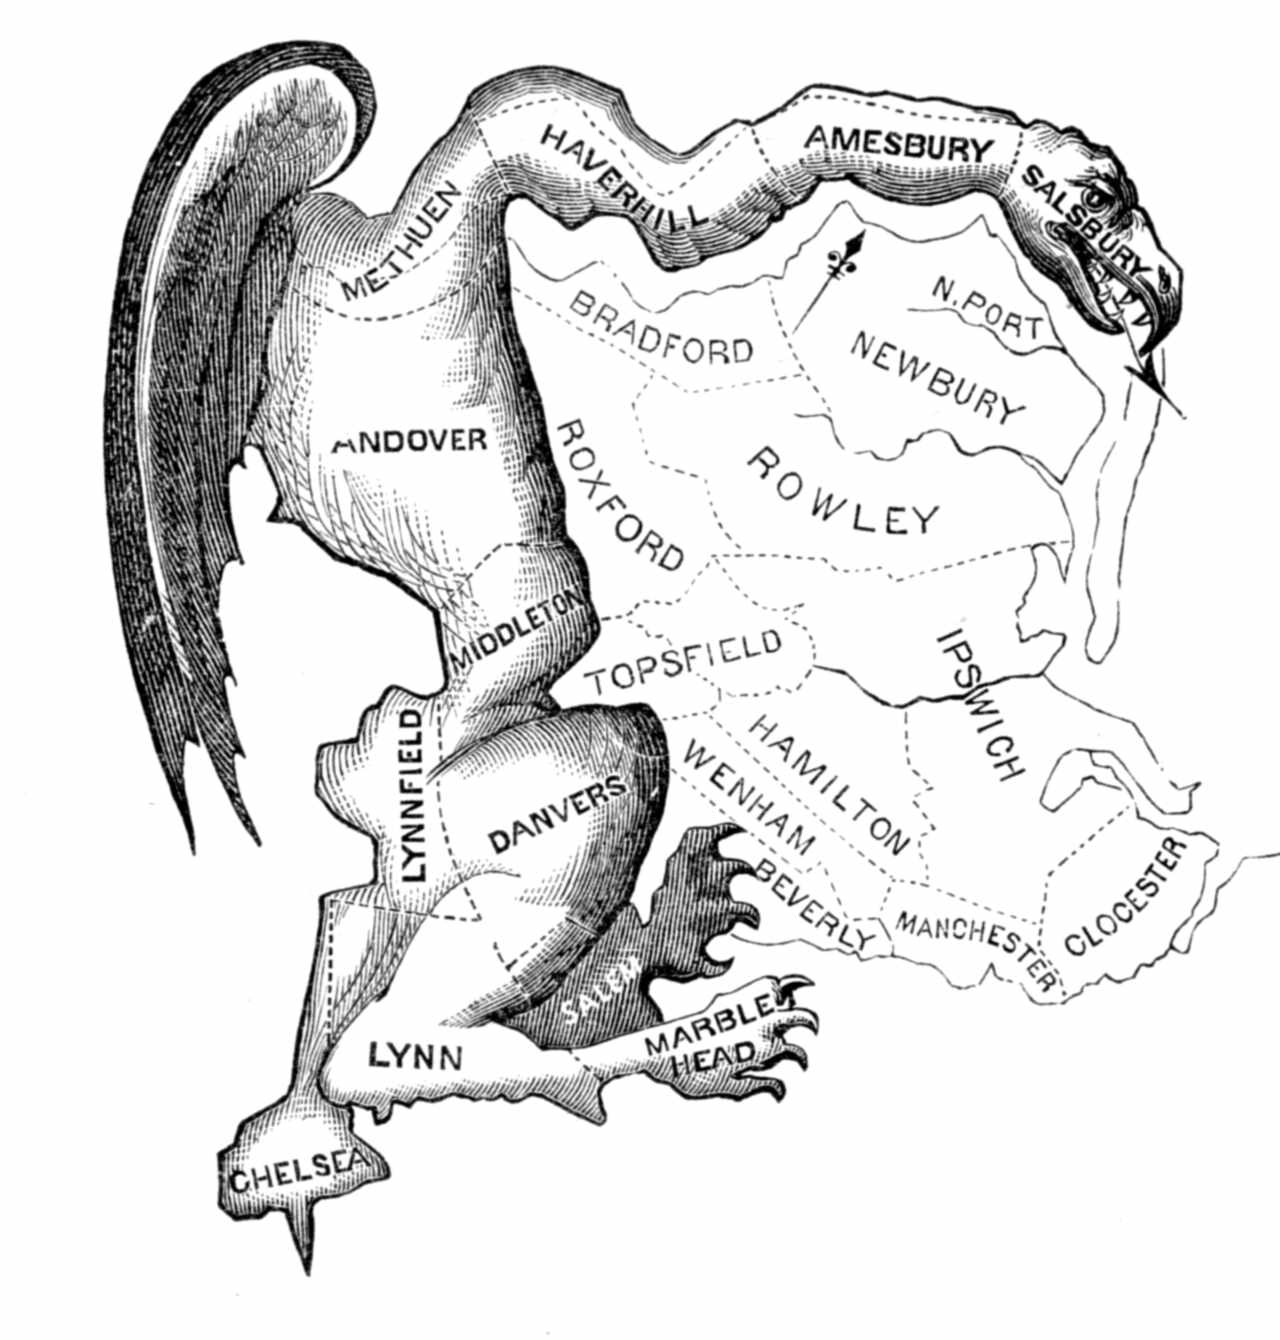
\includegraphics[max width=0.95\textwidth,max height=0.7\textheight]{{Images/gerrymander}.jpg}
\end{center}
\end{column}
\end{columns}
\end{frame}
\subsection{Answers}
\begin{frame}[t]{Round 5 --- Portmanteaus --- \mbox{Answer 1}}
\vspace{-0.5em}
\begin{block}{Question}
What is the name of the annual month-long event during which men grow facial hair in order to raise awareness around men's health issues?
\end{block}

\visible<2->{
    \begin{columns}[T,totalwidth=\linewidth]
    \begin{column}{0.32\linewidth}
    \begin{block}{Answer}
    Movember (mustache + November)
    \end{block}
    \end{column}
    \begin{column}{0.65\linewidth}
    \begin{center}
    
\includegraphics[max height=.45\textheight,
        max width=0.95\textwidth]{{Images/movember}.jpg}
    \end{center}
    \end{column}
    \end{columns}
}
\end{frame}
\begin{frame}[t]{Round 5 --- Portmanteaus --- \mbox{Answer 2}}
\vspace{-0.5em}
\begin{block}{Question}
``Irregardless'', which first appeared in print as early as 1795, is believed to be a portmanteau of which two words with which it is synonymous?
\end{block}
\visible<2->{
    \begin{block}{Answer}
    Irrespective + regardless
    \end{block}
}
\end{frame}
\begin{frame}[t]{Round 5 --- Portmanteaus --- \mbox{Answer 3}}
\vspace{-0.5em}
\begin{block}{Question}
What is the portmanteau term for a period in which high prices and interest rates occur at the same time as high unemployment?
\end{block}

\visible<2->{
    \begin{columns}[T,totalwidth=\linewidth]
    \begin{column}{0.32\linewidth}
    \begin{block}{Answer}
    Stagflation (stagnation + inflation)
    \end{block}
    \end{column}
    \begin{column}{0.65\linewidth}
    \begin{center}
    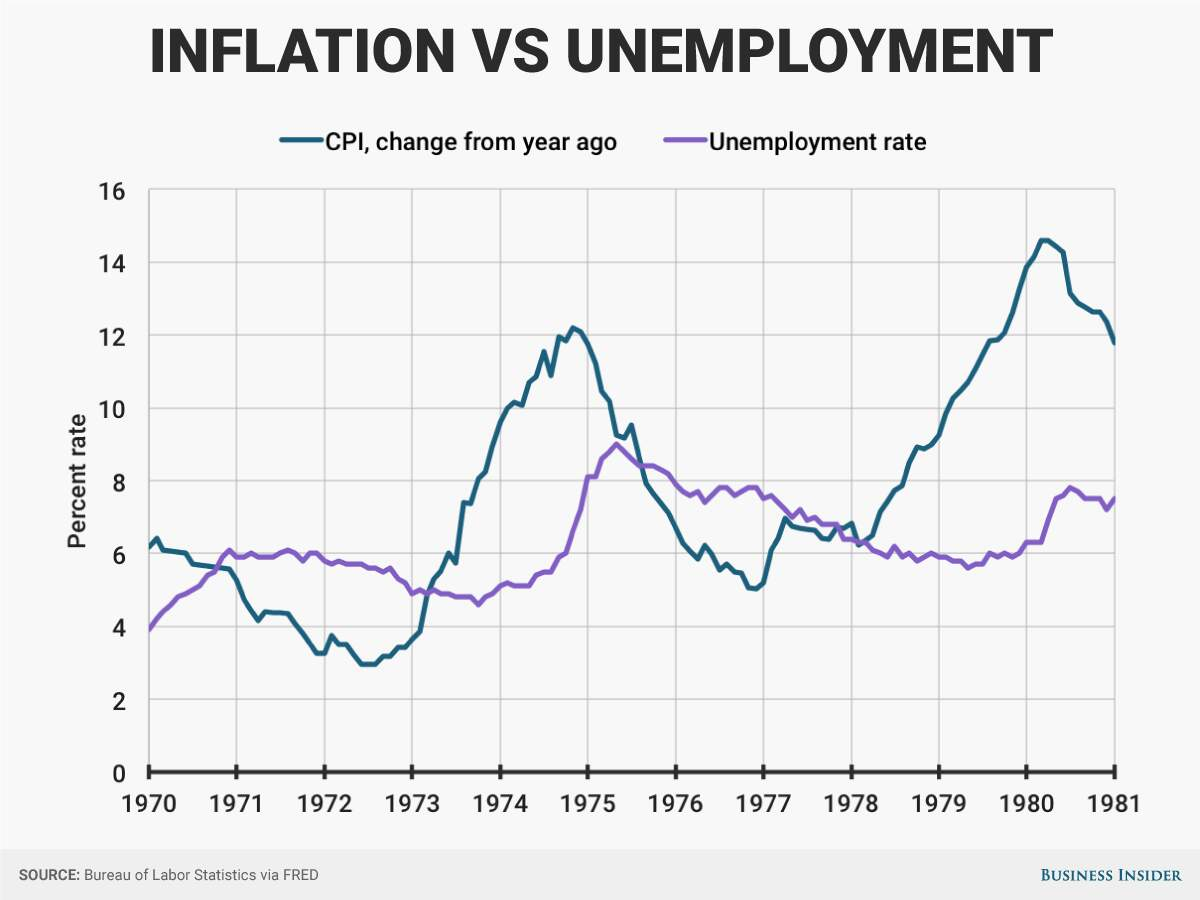
\includegraphics[max height=.45\textheight,
        max width=0.95\textwidth]{{Images/stagflation}.jpg}
    \end{center}
    \end{column}
    \end{columns}
}
\end{frame}
\begin{frame}[t]{Round 5 --- Portmanteaus --- \mbox{Answer 4}}
\vspace{-0.5em}
\begin{block}{Question}
Jim Henson, the creator of the Muppets, coined the word ``muppet'' as a portmanteau of which related two words?
\end{block}

\visible<2->{
    \begin{columns}[T,totalwidth=\linewidth]
    \begin{column}{0.32\linewidth}
    \begin{block}{Answer}
    Marionette + puppet
    \end{block}
    \end{column}
    \begin{column}{0.65\linewidth}
    \begin{center}
    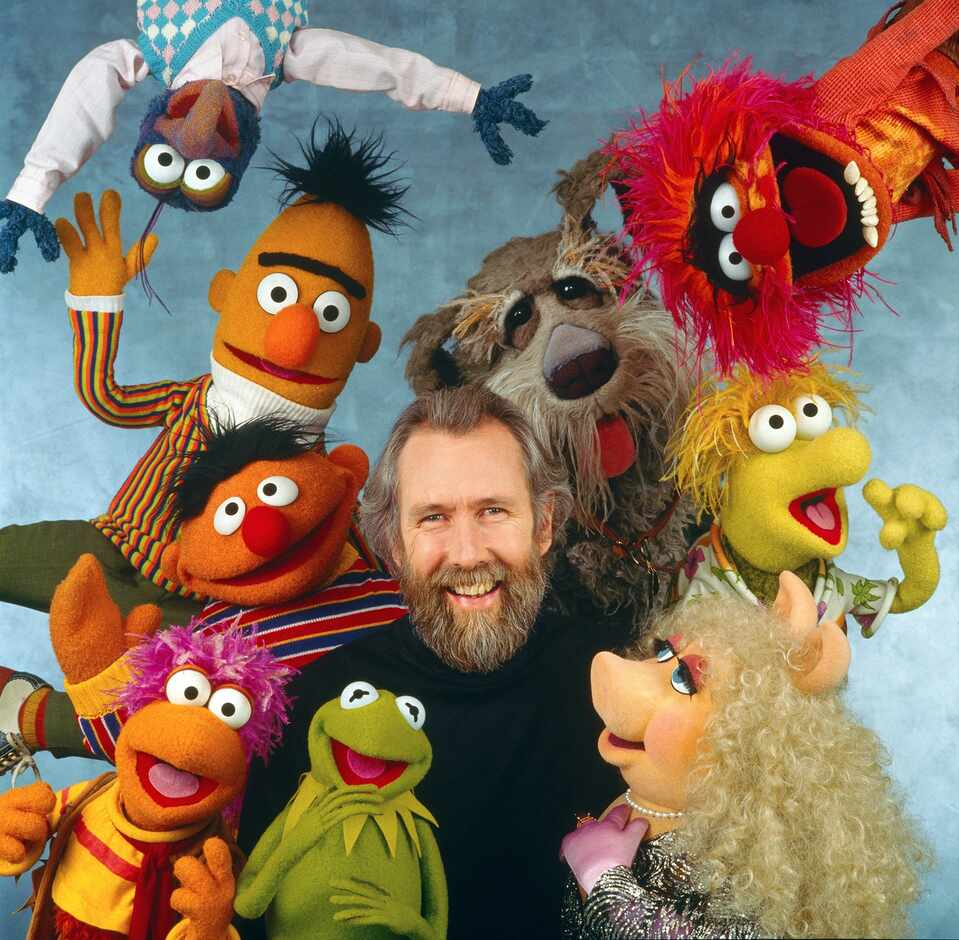
\includegraphics[max height=.45\textheight,
        max width=0.95\textwidth]{{Images/muppets}.jpg}
    \end{center}
    \end{column}
    \end{columns}
}
\end{frame}
\begin{frame}[t]{Round 5 --- Portmanteaus --- \mbox{Answer 5}}
\vspace{-0.5em}
\begin{block}{Question}
What was the portmanteau title of the musical adapted from the film \emph{Monty Python and the Holy Grail}\,?
\end{block}

\visible<2->{
    \begin{columns}[T,totalwidth=\linewidth]
    \begin{column}{0.32\linewidth}
    \begin{block}{Answer}
    \emph{Spamalot} (Spam + Camelot)
    \end{block}
    \end{column}
    \begin{column}{0.65\linewidth}
    \begin{center}
    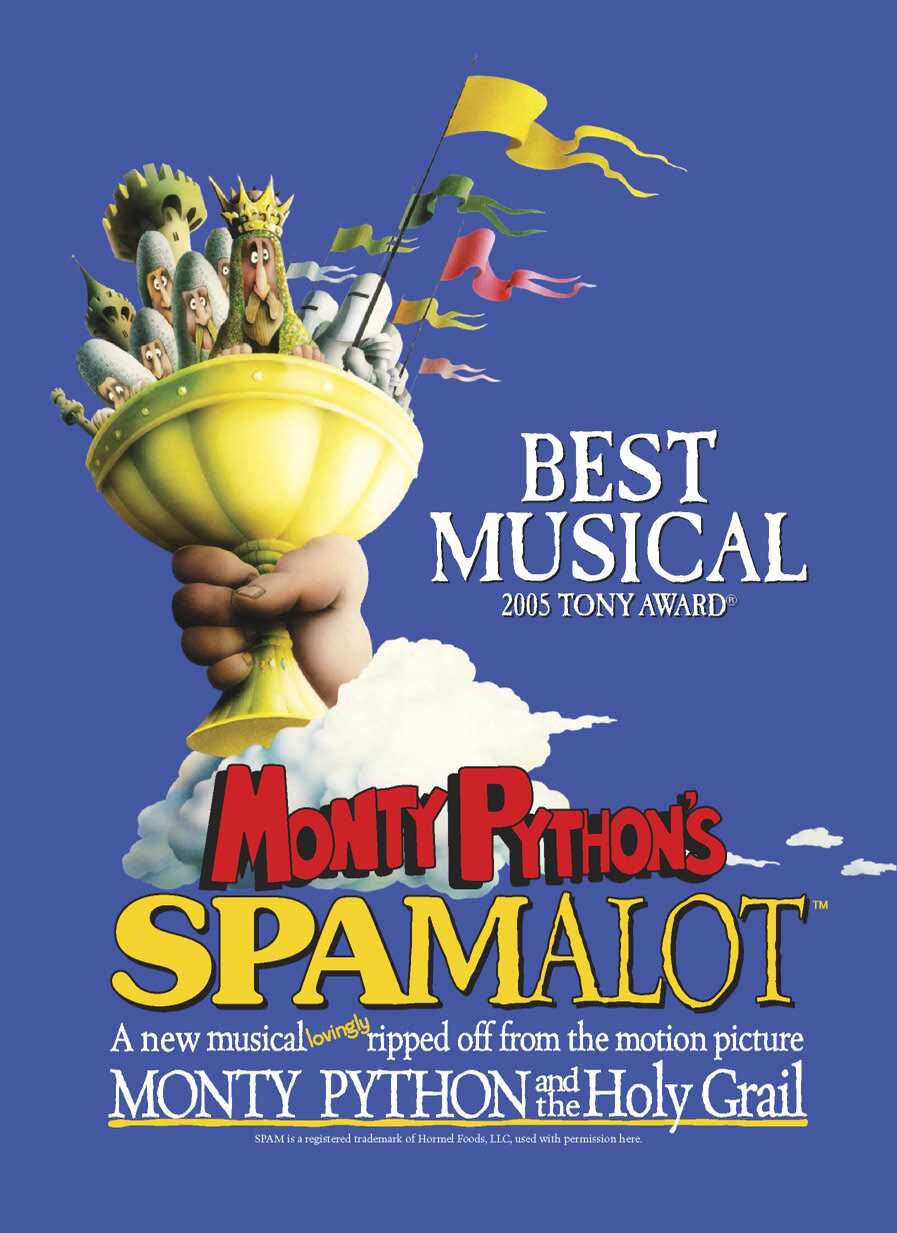
\includegraphics[max height=.45\textheight,
        max width=0.95\textwidth]{{Images/spamalot}.jpg}
    \end{center}
    \end{column}
    \end{columns}
}
\end{frame}
\begin{frame}[t]{Round 5 --- Portmanteaus --- \mbox{Answer 6}}
\vspace{-0.5em}
\begin{block}{Question}
What is the portmanteau word for proper online behavior and manners?
\end{block}
\visible<2->{
    \begin{block}{Answer}
    Netiquette (net + etiquette)
    \end{block}
}
\end{frame}
\begin{frame}[t]{Round 5 --- Portmanteaus --- \mbox{Answer 7}}
\vspace{-0.5em}
\begin{block}{Question}
In computing, the basic unit of information is the bit, which can be either a ``1'' or a ``0''. The word ``bit'' was coined as the portmanteau of which two words?
\end{block}

\visible<2->{
    \begin{columns}[T,totalwidth=\linewidth]
    \begin{column}{0.32\linewidth}
    \begin{block}{Answer}
    Binary + digit
    \end{block}
    \end{column}
    \begin{column}{0.65\linewidth}
    \begin{center}
    \includegraphics[max height=.45\textheight,
        max width=0.95\textwidth]{{Images/bindigit}.jpg}
    \end{center}
    \end{column}
    \end{columns}
}
\end{frame}
\begin{frame}[t]{Round 5 --- Portmanteaus --- \mbox{Answer 8}}
\vspace{-0.5em}
\begin{block}{Question}
If you are perplexed to the point of speechlessness, you could be said to be which portmanteau that is recorded from as early as the 1650s?
\end{block}
\visible<2->{
    \begin{block}{Answer}
    Dumbfounded (dumb + confounded)
    \end{block}
}
\end{frame}
\begin{frame}[t]{Round 5 --- Portmanteaus --- \mbox{Answer 9}}
\vspace{-0.5em}
\begin{block}{Question}
The Flying Spaghetti Monster is the deity of which spoof religion with a portmanteau name?
\end{block}

\visible<2->{
    \begin{columns}[T,totalwidth=\linewidth]
    \begin{column}{0.32\linewidth}
    \begin{block}{Answer}
    Pastafarianism (pasta + Rastafarianism)
    \end{block}
    \end{column}
    \begin{column}{0.65\linewidth}
    \begin{center}
    \includegraphics[max height=.45\textheight,
        max width=0.95\textwidth]{{Images/pastafarian}.jpg}
    \end{center}
    \end{column}
    \end{columns}
}
\end{frame}
\begin{frame}[t]{Round 5 --- Portmanteaus --- \mbox{Answer 10}}
\vspace{-0.5em}
\begin{columns}[T,totalwidth=\linewidth]
    \begin{column}{0.6\linewidth}
    \begin{block}{Question}
    The cartoon shown here was meant to demonstrate the danger of which political practice with a portmanteau name?
    \end{block}
    \end{column}
    \begin{column}{0.38\linewidth}
    \begin{center}
    \includegraphics[max width=0.95\textwidth,
        max height=3in]{{Images/gerrymander}.jpg}
    \end{center}
    \end{column}
\end{columns}

\visible<2->{
    \begin{block}{Answer}
    Gerrymandering (''gerrymander'' being a portmanteau of ``Gerry'', the last name of politician Elbridge Gerry, an early proponent of rigging the shape of electoral districts, and ``salamander'', because the new districts appeared salamander-shaped)
    \end{block}
}
\end{frame}
\def\thisSectionName{``Colorful'' People}
\section{Round 6}
\subsection*{Q1}
\begin{frame}[t]{Round 6 --- ``Colorful'' People --- \mbox{Question 1}}
\vspace{-0.5em}
\begin{block}{Question}
The Rolling Stones asked not to follow what singer with a colorful name in the lineup at 1964's T.A.M.I. Show?
\end{block}
\end{frame}
\subsection*{Q2}
\begin{frame}[t]{Round 6 --- ``Colorful'' People --- \mbox{Question 2}}
\vspace{-0.5em}
\begin{block}{Question}
What 20\textsuperscript{th} century jazz cornet player and bandleader born with the first name ``Ernest'' was better known by his colorful nickname?  (We need both his nickname and his last name.)
\end{block}
\end{frame}
\subsection*{Q3}
\begin{frame}[t]{Round 6 --- ``Colorful'' People --- \mbox{Question 3}}
\vspace{-0.5em}
\begin{block}{Question}
Give the full name of either of the two musicians with colorful names who are part of group The White Stripes.
\end{block}
\end{frame}
\subsection*{Q4}
\begin{frame}[t]{Round 6 --- ``Colorful'' People --- \mbox{Question 4}}
\vspace{-0.5em}
\begin{block}{Question}
What actor with a colorful name starred in the film \emph{School of Rock}?
\end{block}
\end{frame}
\subsection*{Q5}
\begin{frame}[t]{Round 6 --- ``Colorful'' People --- \mbox{Question 5}}
\vspace{-0.5em}
\begin{block}{Question}
What cartoon character with a colorful name has never gotten a ``kick'' out of football?
\end{block}
\end{frame}
\subsection*{Q6}
\begin{frame}[t]{Round 6 --- ``Colorful'' People --- \mbox{Question 6}}
\vspace{-0.5em}
\begin{block}{Question}
What woman with a colorful name has portrayed Black Widow in several Marvel Comics movies?
\end{block}
\end{frame}
\subsection*{Q7}
\begin{frame}[t]{Round 6 --- ``Colorful'' People --- \mbox{Question 7}}
\vspace{-0.5em}
\begin{block}{Question}
The songs of what singer with a colorful name include ``Sober'', ``So What'', and ``What About Us''?
\end{block}
\end{frame}
\subsection*{Q8}
\begin{frame}[t]{Round 6 --- ``Colorful'' People --- \mbox{Question 8}}
\vspace{-0.5em}
\begin{block}{Question}
What NFL player with a colorful name holds the all-time record for rushing yards per game? 
\end{block}
\end{frame}
\subsection*{Q9}
\begin{frame}[t]{Round 6 --- ``Colorful'' People --- \mbox{Question 9}}
\vspace{-0.5em}
\begin{block}{Question}
What pollster with a colorful name runs the FiveThirtyEight?
\end{block}
\end{frame}
\subsection*{Q10}
\begin{frame}[t]{Round 6 --- ``Colorful'' People --- \mbox{Question 10}}
\vspace{-0.5em}
\begin{block}{Question}
Whose colorful name appears in the credits of the film \emph{The Bandwagon} and the Broadway show and film \emph{On the Town}, among many other shows and films?
\end{block}
\end{frame}
\subsection{Answers}
\begin{frame}[t]{Round 6 --- ``Colorful'' People --- \mbox{Answer 1}}
\vspace{-0.5em}
\begin{block}{Question}
The Rolling Stones asked not to follow what singer with a colorful name in the lineup at 1964's T.A.M.I. Show?
\end{block}

\visible<2->{
    \begin{columns}[T,totalwidth=\linewidth]
    \begin{column}{0.32\linewidth}
    \begin{block}{Answer}
    James Brown
    \end{block}
    \end{column}
    \begin{column}{0.65\linewidth}
    \begin{center}
    \includegraphics[max height=.45\textheight,
        max width=0.95\textwidth]{{Images/brown}.jpg}
    \end{center}
    \end{column}
    \end{columns}
}
\end{frame}
\begin{frame}[t]{Round 6 --- ``Colorful'' People --- \mbox{Answer 2}}
\vspace{-0.5em}
\begin{block}{Question}
What 20\textsuperscript{th} century jazz cornet player and bandleader born with the first name ``Ernest'' was better known by his colorful nickname?  (We need both his nickname and his last name.)
\end{block}

\visible<2->{
    \begin{columns}[T,totalwidth=\linewidth]
    \begin{column}{0.32\linewidth}
    \begin{block}{Answer}
    Red Nichols
    \end{block}
    \end{column}
    \begin{column}{0.65\linewidth}
    \begin{center}
    \includegraphics[max height=.45\textheight,
        max width=0.95\textwidth]{{Images/rednichols}.jpeg}
    \end{center}
    \end{column}
    \end{columns}
}
\end{frame}
\begin{frame}[t]{Round 6 --- ``Colorful'' People --- \mbox{Answer 3}}
\vspace{-0.5em}
\begin{block}{Question}
Give the full name of either of the two musicians with colorful names who are part of group The White Stripes.
\end{block}

\visible<2->{
    \begin{columns}[T,totalwidth=\linewidth]
    \begin{column}{0.32\linewidth}
    \begin{block}{Answer}
    Jack White or Meg White (we only needed one)
    \end{block}
    \end{column}
    \begin{column}{0.65\linewidth}
    \begin{center}
    \includegraphics[max height=.45\textheight,
        max width=0.95\textwidth]{{Images/whitestripes}.jpg}
    \end{center}
    \end{column}
    \end{columns}
}
\end{frame}
\begin{frame}[t]{Round 6 --- ``Colorful'' People --- \mbox{Answer 4}}
\vspace{-0.5em}
\begin{block}{Question}
What actor with a colorful name starred in the film \emph{School of Rock}?
\end{block}

\visible<2->{
    \begin{columns}[T,totalwidth=\linewidth]
    \begin{column}{0.32\linewidth}
    \begin{block}{Answer}
    Jack Black
    \end{block}
    \end{column}
    \begin{column}{0.65\linewidth}
    \begin{center}
    \includegraphics[max height=.45\textheight,
        max width=0.95\textwidth]{{Images/sor}.jpg}
    \end{center}
    \end{column}
    \end{columns}
}
\end{frame}
\begin{frame}[t]{Round 6 --- ``Colorful'' People --- \mbox{Answer 5}}
\vspace{-0.5em}
\begin{block}{Question}
What cartoon character with a colorful name has never gotten a ``kick'' out of football?
\end{block}

\visible<2->{
    \begin{columns}[T,totalwidth=\linewidth]
    \begin{column}{0.32\linewidth}
    \begin{block}{Answer}
    Charlie Brown
    \end{block}
    \end{column}
    \begin{column}{0.65\linewidth}
    \begin{center}
    \includegraphics[max height=.45\textheight,
        max width=0.95\textwidth]{{Images/charliebrown}.jpeg}
    \end{center}
    \end{column}
    \end{columns}
}
\end{frame}
\begin{frame}[t]{Round 6 --- ``Colorful'' People --- \mbox{Answer 6}}
\vspace{-0.5em}
\begin{block}{Question}
What woman with a colorful name has portrayed Black Widow in several Marvel Comics movies?
\end{block}

\visible<2->{
    \begin{columns}[T,totalwidth=\linewidth]
    \begin{column}{0.32\linewidth}
    \begin{block}{Answer}
    Scarlett Johansson
    \end{block}
    \end{column}
    \begin{column}{0.65\linewidth}
    \begin{center}
    \includegraphics[max height=.45\textheight,
        max width=0.95\textwidth]{{Images/scarjo}.jpg}
    \end{center}
    \end{column}
    \end{columns}
}
\end{frame}
\begin{frame}[t]{Round 6 --- ``Colorful'' People --- \mbox{Answer 7}}
\vspace{-0.5em}
\begin{block}{Question}
The songs of what singer with a colorful name include ``Sober'', ``So What'', and ``What About Us''?
\end{block}

\visible<2->{
    \begin{columns}[T,totalwidth=\linewidth]
    \begin{column}{0.32\linewidth}
    \begin{block}{Answer}
    P!nk / Pink
    \end{block}
    \end{column}
    \begin{column}{0.65\linewidth}
    \begin{center}
    \includegraphics[max height=.45\textheight,
        max width=0.95\textwidth]{{Images/pink}.jpg}
    \end{center}
    \end{column}
    \end{columns}
}
\end{frame}
\begin{frame}[t]{Round 6 --- ``Colorful'' People --- \mbox{Answer 8}}
\vspace{-0.5em}
\begin{block}{Question}
What NFL player with a colorful name holds the all-time record for rushing yards per game? 
\end{block}

\visible<2->{
    \begin{columns}[T,totalwidth=\linewidth]
    \begin{column}{0.32\linewidth}
    \begin{block}{Answer}
    Jim Brown (104.3 yards per game)
    \end{block}
    \end{column}
    \begin{column}{0.65\linewidth}
    \begin{center}
    \includegraphics[max height=.45\textheight,
        max width=0.95\textwidth]{{Images/jimbrown}.jpg}
    \end{center}
    \end{column}
    \end{columns}
}
\end{frame}
\begin{frame}[t]{Round 6 --- ``Colorful'' People --- \mbox{Answer 9}}
\vspace{-0.5em}
\begin{block}{Question}
What pollster with a colorful name runs the FiveThirtyEight?
\end{block}

\visible<2->{
    \begin{columns}[T,totalwidth=\linewidth]
    \begin{column}{0.32\linewidth}
    \begin{block}{Answer}
    Nate Silver
    \end{block}
    \end{column}
    \begin{column}{0.65\linewidth}
    \begin{center}
    \includegraphics[max height=.45\textheight,
        max width=0.95\textwidth]{{Images/natesilver}.jpg}
    \end{center}
    \end{column}
    \end{columns}
}
\end{frame}
\begin{frame}[t]{Round 6 --- ``Colorful'' People --- \mbox{Answer 10}}
\vspace{-0.5em}
\begin{block}{Question}
Whose colorful name appears in the credits of the film \emph{The Bandwagon} and the Broadway show and film \emph{On the Town}, among many other shows and films?
\end{block}

\visible<2->{
    \begin{columns}[T,totalwidth=\linewidth]
    \begin{column}{0.32\linewidth}
    \begin{block}{Answer}
    Adolph Green
    \end{block}
    \end{column}
    \begin{column}{0.65\linewidth}
    \begin{center}
    \includegraphics[max height=.45\textheight,
        max width=0.95\textwidth]{{Images/adolphgreen}.jpg}
    \end{center}
    \end{column}
    \end{columns}
}
\end{frame}
\begin{frame}
\includegraphics[max width=\textwidth,max height=\textheight]{Images/jeopardygreen.jpg}
\end{frame}
\begin{frame}
\includegraphics[max width=\textwidth,max height=\textheight]{Images/howard.jpg}
\end{frame}
\def\thisSectionName{Booze Clues}
\section{Round 7}
\subsection*{Q1}
\begin{frame}[t]{Round 7 --- Booze Clues --- \mbox{Question 1}}
\vspace{-0.5em}
\begin{block}{Question}
What substance is fermented to produce mead?
\end{block}
\end{frame}
\subsection*{Q2}
\begin{frame}[t]{Round 7 --- Booze Clues --- \mbox{Question 2}}
\vspace{-0.5em}
\begin{block}{Question}
What is the colloquial name of the plant with the scientific name \emph{Artemisia absinthium}, which is used to make absinthe?
\end{block}
\end{frame}
\subsection*{Q3}
\begin{frame}[t]{Round 7 --- Booze Clues --- \mbox{Question 3}}
\vspace{-0.5em}
\begin{block}{Question}
Which country does \emph{ouzo}, an anise-flavored aperitif, come from?
\end{block}
\end{frame}
\subsection*{Q4}
\begin{frame}[t]{Round 7 --- Booze Clues --- \mbox{Question 4}}
\vspace{-0.5em}
\begin{block}{Question}
Even after the repeal of Prohibition, people continued to illegally make moonshine and moonshiners continued to evade federal agents, who they called ``revenuers''. What job did revenuers perform?
\end{block}
\end{frame}
\subsection*{Q5}
\begin{frame}[t]{Round 7 --- Booze Clues --- \mbox{Question 5}}
\vspace{-0.5em}
\begin{block}{Question}
In Slavic languages, ``vodka'' is the diminutive of ``voda''. What does ``voda'' mean in English?
\end{block}
\end{frame}
\subsection*{Q6}
\begin{frame}[t]{Round 7 --- Booze Clues --- \mbox{Question 6}}
\vspace{-0.5em}
\begin{block}{Question}
What is the chemical formula of ethanol, the thing that gives booze its kick?
\end{block}
\end{frame}
\subsection*{Q7}
\begin{frame}[t]{Round 7 --- Booze Clues --- \mbox{Question 7}}
\vspace{-0.5em}
\begin{block}{Question}
In which country are the grapes used to make sherry grown?
\end{block}
\end{frame}
\subsection*{Q8}
\begin{frame}[t]{Round 7 --- Booze Clues --- \mbox{Question 8}}
\vspace{-0.5em}
\begin{block}{Question}
What fruit gives gin its flavor?
\end{block}
\end{frame}
\subsection*{Q9}
\begin{frame}[t]{Round 7 --- Booze Clues --- \mbox{Question 9}}
\vspace{-0.5em}
\begin{block}{Question}
What is the name of the apparatus in which the process of precisely boiling and condensing a liquid mixture in order to separate its components --- a process ubiquitous in the production of alcohol --- is performed?
\end{block}
\end{frame}
\subsection*{Q10}
\begin{frame}[t]{Round 7 --- Booze Clues --- \mbox{Question 10}}
\vspace{-0.5em}
\begin{block}{Question}
Who said of drinking: ``I feel bad for people who don't drink. When they wake up in the morning, that's as good as they're going to feel all day''?
\end{block}
\end{frame}
\subsection{Answers}
\begin{frame}[t]{Round 7 --- Booze Clues --- \mbox{Answer 1}}
\vspace{-0.5em}
\begin{block}{Question}
What substance is fermented to produce mead?
\end{block}

\visible<2->{
    \begin{columns}[T,totalwidth=\linewidth]
    \begin{column}{0.32\linewidth}
    \begin{block}{Answer}
    Honey
    \end{block}
    \end{column}
    \begin{column}{0.65\linewidth}
    \begin{center}
    \includegraphics[max height=.45\textheight,
        max width=0.95\textwidth]{{Images/honey}.jpg}
    \end{center}
    \end{column}
    \end{columns}
}
\end{frame}
\begin{frame}[t]{Round 7 --- Booze Clues --- \mbox{Answer 2}}
\vspace{-0.5em}
\begin{block}{Question}
What is the colloquial name of the plant with the scientific name \emph{Artemisia absinthium}, which is used to make absinthe?
\end{block}

\visible<2->{
    \begin{columns}[T,totalwidth=\linewidth]
    \begin{column}{0.32\linewidth}
    \begin{block}{Answer}
    Wormwood / mugwort
    \end{block}
    \end{column}
    \begin{column}{0.65\linewidth}
    \begin{center}
    \includegraphics[max height=.45\textheight,
        max width=0.95\textwidth]{{Images/absinthia}.jpg}
    \end{center}
    \end{column}
    \end{columns}
}
\end{frame}
\begin{frame}[t]{Round 7 --- Booze Clues --- \mbox{Answer 3}}
\vspace{-0.5em}
\begin{block}{Question}
Which country does \emph{ouzo}, an anise-flavored aperitif, come from?
\end{block}

\visible<2->{
    \begin{columns}[T,totalwidth=\linewidth]
    \begin{column}{0.32\linewidth}
    \begin{block}{Answer}
    Greece / Cyprus
    \end{block}
    \end{column}
    \begin{column}{0.65\linewidth}
    \begin{center}
    \includegraphics[max height=.45\textheight,
        max width=0.95\textwidth]{{Images/ouzo}.jpeg}
    \end{center}
    \end{column}
    \end{columns}
}
\end{frame}
\begin{frame}[t]{Round 7 --- Booze Clues --- \mbox{Answer 4}}
\vspace{-0.5em}
\begin{block}{Question}
Even after the repeal of Prohibition, people continued to illegally make moonshine and moonshiners continued to evade federal agents, who they called ``revenuers''. What job did revenuers perform?
\end{block}

\visible<2->{
    \begin{columns}[T,totalwidth=\linewidth]
    \begin{column}{0.32\linewidth}
    \begin{block}{Answer}
    Collecting taxes on alcohol (which moonshiners attempted to avoid paying)
    \end{block}
    \end{column}
    \begin{column}{0.65\linewidth}
    \begin{center}
    \includegraphics[max height=.45\textheight,
        max width=0.95\textwidth]{{Images/moonshine}.jpeg}
    \end{center}
    \end{column}
    \end{columns}
}
\end{frame}
\begin{frame}[t]{Round 7 --- Booze Clues --- \mbox{Answer 5}}
\vspace{-0.5em}
\begin{block}{Question}
In Slavic languages, ``vodka'' is the diminutive of ``voda''. What does ``voda'' mean in English?
\end{block}
\visible<2->{
    \begin{block}{Answer}
    Water
    \end{block}
}
\end{frame}
\begin{frame}[t]{Round 7 --- Booze Clues --- \mbox{Answer 6}}
\vspace{-0.5em}
\begin{block}{Question}
What is the chemical formula of ethanol, the thing that gives booze its kick?
\end{block}

\visible<2->{
    \begin{columns}[T,totalwidth=\linewidth]
    \begin{column}{0.32\linewidth}
    \begin{block}{Answer}
    \ch{C2H6O} / \ch{C2H5OH} (we'll also accept any answer containing the correct number of each element, regardless of how it's written)
    \end{block}
    \end{column}
    \begin{column}{0.65\linewidth}
    \begin{center}
    \includegraphics[max height=.45\textheight,
        max width=0.95\textwidth]{{Images/ethanol}.jpg}
    \end{center}
    \end{column}
    \end{columns}
}
\end{frame}
\begin{frame}[t]{Round 7 --- Booze Clues --- \mbox{Answer 7}}
\vspace{-0.5em}
\begin{block}{Question}
In which country are the grapes used to make sherry grown?
\end{block}

\visible<2->{
    \begin{columns}[T,totalwidth=\linewidth]
    \begin{column}{0.32\linewidth}
    \begin{block}{Answer}
    Spain
    \end{block}
    \end{column}
    \begin{column}{0.65\linewidth}
    \begin{center}
    \includegraphics[max height=.45\textheight,
        max width=0.95\textwidth]{{Images/sherry}.jpg}
    \end{center}
    \end{column}
    \end{columns}
}
\end{frame}
\begin{frame}[t]{Round 7 --- Booze Clues --- \mbox{Answer 8}}
\vspace{-0.5em}
\begin{block}{Question}
What fruit gives gin its flavor?
\end{block}

\visible<2->{
    \begin{columns}[T,totalwidth=\linewidth]
    \begin{column}{0.32\linewidth}
    \begin{block}{Answer}
    Juniper berries
    \end{block}
    \end{column}
    \begin{column}{0.65\linewidth}
    \begin{center}
    \includegraphics[max height=.45\textheight,
        max width=0.95\textwidth]{{Images/juniper}.jpg}
    \end{center}
    \end{column}
    \end{columns}
}
\end{frame}
\begin{frame}[t]{Round 7 --- Booze Clues --- \mbox{Answer 9}}
\vspace{-0.5em}
\begin{block}{Question}
What is the name of the apparatus in which the process of precisely boiling and condensing a liquid mixture in order to separate its components --- a process ubiquitous in the production of alcohol --- is performed?
\end{block}

\visible<2->{
    \begin{columns}[T,totalwidth=\linewidth]
    \begin{column}{0.32\linewidth}
    \begin{block}{Answer}
    A still
    \end{block}
    \end{column}
    \begin{column}{0.65\linewidth}
    \begin{center}
    \includegraphics[max height=.45\textheight,
        max width=0.95\textwidth]{{Images/still}.jpeg}
    \end{center}
    \end{column}
    \end{columns}
}
\end{frame}
\begin{frame}[t]{Round 7 --- Booze Clues --- \mbox{Answer 10}}
\vspace{-0.5em}
\begin{block}{Question}
Who said of drinking: ``I feel bad for people who don't drink. When they wake up in the morning, that's as good as they're going to feel all day''?
\end{block}

\visible<2->{
    \begin{columns}[T,totalwidth=\linewidth]
    \begin{column}{0.32\linewidth}
    \begin{block}{Answer}
    Dean Martin / Frank Sinatra (when Sinatra said it, he was quoting Dean Martin)
    \end{block}
    \end{column}
    \begin{column}{0.65\linewidth}
    \begin{center}
    \includegraphics[max height=.45\textheight,
        max width=0.95\textwidth]{{Images/sinatra}.jpg}
    \end{center}
    \end{column}
    \end{columns}
}
\end{frame}
\def\thisSectionName{NPR and PBS}
\section{Round 8}
\subsection*{Q1}
\begin{frame}[t]{Round 8 --- NPR and PBS --- \mbox{Question 1}}
\vspace{-0.5em}
\begin{block}{Question}
What was the full title of the PBS documentary series that documented the life of the Loud family?
\end{block}
\end{frame}
\subsection*{Q2}
\begin{frame}[t]{Round 8 --- NPR and PBS --- \mbox{Question 2}}
\vspace{-0.5em}
\begin{block}{Question}
What was the last name of the two brothers who hosted a car repair show on NPR for many years?
\end{block}
\end{frame}
\subsection*{Q3}
\begin{frame}[t]{Round 8 --- NPR and PBS --- \mbox{Question 3}}
\vspace{-0.5em}
\begin{block}{Question}
What was the full name of the long-running PBS children's show that was hosted by a Presbyterian minister?
\end{block}
\end{frame}
\subsection*{Q4}
\begin{frame}[t]{Round 8 --- NPR and PBS --- \mbox{Question 4}}
\vspace{-0.5em}
\begin{block}{Question}
In what year did \emph{Sesame Street} first go on the air?
\end{block}
\end{frame}
\subsection*{Q5}
\begin{frame}[t]{Round 8 --- NPR and PBS --- \mbox{Question 5}}
\vspace{-0.5em}
\begin{block}{Question}
What is the name of the NPR weekly comedy news quiz?
\end{block}
\end{frame}
\subsection*{Q6}
\begin{frame}[t]{Round 8 --- NPR and PBS --- \mbox{Question 6}}
\vspace{-0.5em}
\begin{block}{Question}
What is the name of  NPR's morning news show? 
\end{block}
\end{frame}
\subsection*{Q7}
\begin{frame}[t]{Round 8 --- NPR and PBS --- \mbox{Question 7}}
\vspace{-0.5em}
\begin{block}{Question}
Who is the host of the NPR interview show \emph{Fresh Air}?
\end{block}
\end{frame}
\subsection*{Q8}
\begin{frame}[t]{Round 8 --- NPR and PBS --- \mbox{Question 8}}
\vspace{-0.5em}
\begin{block}{Question}
Which European broadcaster's news shows are carried by NPR\@?
\end{block}
\end{frame}
\subsection*{Q9}
\begin{frame}[t]{Round 8 --- NPR and PBS --- \mbox{Question 9}}
\vspace{-0.5em}
\begin{block}{Question}
What PBS show features serialized British dramas?
\end{block}
\end{frame}
\subsection*{Q10}
\begin{frame}[t]{Round 8 --- NPR and PBS --- \mbox{Question 10}}
\vspace{-0.5em}
\begin{block}{Question}
Who was the original host of the PBS science series \emph{Cosmos}?
\end{block}
\end{frame}
\subsection{Answers}
\begin{frame}[t]{Round 8 --- NPR and PBS --- \mbox{Answer 1}}
\vspace{-0.5em}
\begin{block}{Question}
What was the full title of the PBS documentary series that documented the life of the Loud family?
\end{block}

\visible<2->{
    \begin{columns}[T,totalwidth=\linewidth]
    \begin{column}{0.32\linewidth}
    \begin{block}{Answer}
    \emph{An American Family} (we needed the exact title)
    \end{block}
    \end{column}
    \begin{column}{0.65\linewidth}
    \begin{center}
    \includegraphics[max height=.45\textheight,
        max width=0.95\textwidth]{{Images/americanfamily}.JPG}
    \end{center}
    \end{column}
    \end{columns}
}
\end{frame}
\begin{frame}[t]{Round 8 --- NPR and PBS --- \mbox{Answer 2}}
\vspace{-0.5em}
\begin{block}{Question}
What was the last name of the two brothers who hosted a car repair show on NPR for many years?
\end{block}

\visible<2->{
    \begin{columns}[T,totalwidth=\linewidth]
    \begin{column}{0.32\linewidth}
    \begin{block}{Answer}
    Magliozzi (Tom and Ray)
    \end{block}
    \end{column}
    \begin{column}{0.65\linewidth}
    \begin{center}
    \includegraphics[max height=.45\textheight,
        max width=0.95\textwidth]{{Images/cartalk}.jpg}
    \end{center}
    \end{column}
    \end{columns}
}
\end{frame}
\begin{frame}[t]{Round 8 --- NPR and PBS --- \mbox{Answer 3}}
\vspace{-0.5em}
\begin{block}{Question}
What was the full name of the long-running PBS children's show that was hosted by a Presbyterian minister?
\end{block}

\visible<2->{
    \begin{columns}[T,totalwidth=\linewidth]
    \begin{column}{0.32\linewidth}
    \begin{block}{Answer}
    \emph{Mister Rogers' Neighborhood} (spelling / apostrophization not important) 
    \end{block}
    \end{column}
    \begin{column}{0.65\linewidth}
    \begin{center}
    \includegraphics[max height=.45\textheight,
        max width=0.95\textwidth]{{Images/mrrogers}.jpg}
    \end{center}
    \end{column}
    \end{columns}
}
\end{frame}
\begin{frame}[t]{Round 8 --- NPR and PBS --- \mbox{Answer 4}}
\vspace{-0.5em}
\begin{block}{Question}
In what year did \emph{Sesame Street} first go on the air?
\end{block}

\visible<2->{
    \begin{columns}[T,totalwidth=\linewidth]
    \begin{column}{0.32\linewidth}
    \begin{block}{Answer}
    1969
    \end{block}
    \end{column}
    \begin{column}{0.65\linewidth}
    \begin{center}
    \includegraphics[max height=.45\textheight,
        max width=0.95\textwidth]{{Images/sesame}.jpg}
    \end{center}
    \end{column}
    \end{columns}
}
\end{frame}
\begin{frame}[t]{Round 8 --- NPR and PBS --- \mbox{Answer 5}}
\vspace{-0.5em}
\begin{block}{Question}
What is the name of the NPR weekly comedy news quiz?
\end{block}

\visible<2->{
    \begin{columns}[T,totalwidth=\linewidth]
    \begin{column}{0.32\linewidth}
    \begin{block}{Answer}
    \emph{Wait Wait...Don't Tell Me!}
    \end{block}
    \end{column}
    \begin{column}{0.65\linewidth}
    \begin{center}
    \includegraphics[max height=.45\textheight,
        max width=0.95\textwidth]{{Images/waitwait}.jpeg}
    \end{center}
    \end{column}
    \end{columns}
}
\end{frame}
\begin{frame}[t]{Round 8 --- NPR and PBS --- \mbox{Answer 6}}
\vspace{-0.5em}
\begin{block}{Question}
What is the name of  NPR's morning news show? 
\end{block}

\visible<2->{
    \begin{columns}[T,totalwidth=\linewidth]
    \begin{column}{0.32\linewidth}
    \begin{block}{Answer}
    \emph{Morning Edition}
    \end{block}
    \end{column}
    \begin{column}{0.65\linewidth}
    \begin{center}
    \includegraphics[max height=.45\textheight,
        max width=0.95\textwidth]{{Images/morningedition}.jpeg}
    \end{center}
    \end{column}
    \end{columns}
}
\end{frame}
\begin{frame}[t]{Round 8 --- NPR and PBS --- \mbox{Answer 7}}
\vspace{-0.5em}
\begin{block}{Question}
Who is the host of the NPR interview show \emph{Fresh Air}?
\end{block}

\visible<2->{
    \begin{columns}[T,totalwidth=\linewidth]
    \begin{column}{0.32\linewidth}
    \begin{block}{Answer}
    Terry Gross
    \end{block}
    \end{column}
    \begin{column}{0.65\linewidth}
    \begin{center}
    \includegraphics[max height=.45\textheight,
        max width=0.95\textwidth]{{Images/gross}.jpg}
    \end{center}
    \end{column}
    \end{columns}
}
\end{frame}
\begin{frame}[t]{Round 8 --- NPR and PBS --- \mbox{Answer 8}}
\vspace{-0.5em}
\begin{block}{Question}
Which European broadcaster's news shows are carried by NPR\@?
\end{block}
\visible<2->{
    \begin{block}{Answer}
    The BBC (British Broadcasting Corporation)
    \end{block}
}
\end{frame}
\begin{frame}[t]{Round 8 --- NPR and PBS --- \mbox{Answer 9}}
\vspace{-0.5em}
\begin{block}{Question}
What PBS show features serialized British dramas?
\end{block}

\visible<2->{
    \begin{columns}[T,totalwidth=\linewidth]
    \begin{column}{0.32\linewidth}
    \begin{block}{Answer}
    \emph{Masterpiece} / \emph{Masterpiece Theater}
    \end{block}
    \end{column}
    \begin{column}{0.65\linewidth}
    \begin{center}
    \includegraphics[max height=.45\textheight,
        max width=0.95\textwidth]{{Images/masterpiece}.jpg}
    \end{center}
    \end{column}
    \end{columns}
}
\end{frame}
\begin{frame}[t]{Round 8 --- NPR and PBS --- \mbox{Answer 10}}
\vspace{-0.5em}
\begin{block}{Question}
Who was the original host of the PBS science series \emph{Cosmos}?
\end{block}

\visible<2->{
    \begin{columns}[T,totalwidth=\linewidth]
    \begin{column}{0.32\linewidth}
    \begin{block}{Answer}
    Carl Sagan
    \end{block}
    \end{column}
    \begin{column}{0.65\linewidth}
    \begin{center}
    \includegraphics[max height=.45\textheight,
        max width=0.95\textwidth]{{Images/sagan}.jpeg}
    \end{center}
    \end{column}
    \end{columns}
}
\end{frame}
\def\thisSectionName{Tales and Fables}
\section{Round 9}
\subsection*{Q1}
\begin{frame}[t]{Round 9 --- Tales and Fables --- \mbox{Question 1}}
\vspace{-0.5em}
\begin{block}{Question}
The very first fairy tale printed in English --- in 1621 --- was about which diminutive boy?
\end{block}
\end{frame}
\subsection*{Q2}
\begin{frame}[t]{Round 9 --- Tales and Fables --- \mbox{Question 2}}
\vspace{-0.5em}
\begin{block}{Question}
The 1740 French fairy tale \emph{La Belle et la B{\^ e}te} is known by what title in English?
\end{block}
\end{frame}
\subsection*{Q3}
\begin{frame}[t]{Round 9 --- Tales and Fables --- \mbox{Question 3}}
\vspace{-0.5em}
\begin{block}{Question}
Which classic fairytale was the animated Disney film \emph{Tangled} based on?
\end{block}
\end{frame}
\subsection*{Q4}
\begin{frame}[t]{Round 9 --- Tales and Fables --- \mbox{Question 4}}
\vspace{-0.5em}
\begin{block}{Question}
Fill in both blanks: ``Whoso Pulleth Out This \textunderscore{}\textunderscore{}\textunderscore{}\textunderscore{}\textunderscore{} of this \textunderscore{}\textunderscore{}\textunderscore{}\textunderscore{}\textunderscore{} and Anvil, is Rightwise King Born of all England.''
\end{block}
\end{frame}
\subsection*{Q5}
\begin{frame}[t]{Round 9 --- Tales and Fables --- \mbox{Question 5}}
\vspace{-0.5em}
\begin{block}{Question}
In the tale of Rumpelstiltskin, what supernatural ability does the titular character possess?
\end{block}
\end{frame}
\subsection*{Q6}
\begin{frame}[t]{Round 9 --- Tales and Fables --- \mbox{Question 6}}
\vspace{-0.5em}
\begin{block}{Question}
Who is regarded as the author of the tale of \emph{The Boy Who Cried Wolf}\,?
\end{block}
\end{frame}
\subsection*{Q7}
\begin{frame}[t]{Round 9 --- Tales and Fables --- \mbox{Question 7}}
\vspace{-0.5em}
\begin{block}{Question}
Name six of the seven dwarves in \emph{Snow White}.
\end{block}
\end{frame}
\subsection*{Q8}
\begin{frame}[t]{Round 9 --- Tales and Fables --- \mbox{Question 8}}
\vspace{-0.5em}
\begin{block}{Question}
Fill in the last five words of this well-known quatrain from \emph{Jack and the Beanstalk}:
\begin{quotation}
Fee-fi-fo-fum, \\
I smell the blood of an Englishman, \\
Be he alive, or be he dead \\
I'll grind his \textunderscore{}\textunderscore{}\textunderscore{}\textunderscore{}\textunderscore{} \textunderscore{}\textunderscore{}\textunderscore{}\textunderscore{}\textunderscore{} \textunderscore{}\textunderscore{}\textunderscore{}\textunderscore{}\textunderscore{} \textunderscore{}\textunderscore{}\textunderscore{}\textunderscore{}\textunderscore{} \textunderscore{}\textunderscore{}\textunderscore{}\textunderscore{}\textunderscore{}.
\end{quotation}
\end{block}
\end{frame}
\subsection*{Q9}
\begin{frame}[t]{Round 9 --- Tales and Fables --- \mbox{Question 9}}
\vspace{-0.5em}
\begin{block}{Question}
Who wrote the original \emph{The Little Mermaid} story, on which the 1989 Disney film was based?
\end{block}
\end{frame}
\subsection*{Q10}
\begin{frame}[t]{Round 9 --- Tales and Fables --- \mbox{Question 10}}
\vspace{-0.5em}
\begin{block}{Question}
Scheherazade is the storyteller and a major character in which collection of folk tales?
\end{block}
\end{frame}
\subsection{Answers}
\begin{frame}[t]{Round 9 --- Tales and Fables --- \mbox{Answer 1}}
\vspace{-0.5em}
\begin{block}{Question}
The very first fairy tale printed in English --- in 1621 --- was about which diminutive boy?
\end{block}

\visible<2->{
    \begin{columns}[T,totalwidth=\linewidth]
    \begin{column}{0.32\linewidth}
    \begin{block}{Answer}
    Tom Thumb
    \end{block}
    \end{column}
    \begin{column}{0.65\linewidth}
    \begin{center}
    \includegraphics[max height=.45\textheight,
        max width=0.95\textwidth]{{Images/tomthumb}.jpg}
    \end{center}
    \end{column}
    \end{columns}
}
\end{frame}
\begin{frame}[t]{Round 9 --- Tales and Fables --- \mbox{Answer 2}}
\vspace{-0.5em}
\begin{block}{Question}
The 1740 French fairy tale \emph{La Belle et la B{\^ e}te} is known by what title in English?
\end{block}

\visible<2->{
    \begin{columns}[T,totalwidth=\linewidth]
    \begin{column}{0.32\linewidth}
    \begin{block}{Answer}
    \emph{Beauty and the Beast}
    \end{block}
    \end{column}
    \begin{column}{0.65\linewidth}
    \begin{center}
    \includegraphics[max height=.45\textheight,
        max width=0.95\textwidth]{{Images/beautybeast}.jpeg}
    \end{center}
    \end{column}
    \end{columns}
}
\end{frame}
\begin{frame}[t]{Round 9 --- Tales and Fables --- \mbox{Answer 3}}
\vspace{-0.5em}
\begin{block}{Question}
Which classic fairytale was the animated Disney film \emph{Tangled} based on?
\end{block}

\visible<2->{
    \begin{columns}[T,totalwidth=\linewidth]
    \begin{column}{0.32\linewidth}
    \begin{block}{Answer}
    Rapunzel
    \end{block}
    \end{column}
    \begin{column}{0.65\linewidth}
    \begin{center}
    \includegraphics[max height=.45\textheight,
        max width=0.95\textwidth]{{Images/tangled}.jpg}
    \end{center}
    \end{column}
    \end{columns}
}
\end{frame}
\begin{frame}[t]{Round 9 --- Tales and Fables --- \mbox{Answer 4}}
\vspace{-0.5em}
\begin{block}{Question}
Fill in both blanks: ``Whoso Pulleth Out This \textunderscore{}\textunderscore{}\textunderscore{}\textunderscore{}\textunderscore{} of this \textunderscore{}\textunderscore{}\textunderscore{}\textunderscore{}\textunderscore{} and Anvil, is Rightwise King Born of all England.''
\end{block}

\visible<2->{
    \begin{columns}[T,totalwidth=\linewidth]
    \begin{column}{0.32\linewidth}
    \begin{block}{Answer}
    Sword and stone (from Le Morte d'Arthur)
    \end{block}
    \end{column}
    \begin{column}{0.65\linewidth}
    \begin{center}
    \includegraphics[max height=.45\textheight,
        max width=0.95\textwidth]{{Images/kingarthur}.jpg}
    \end{center}
    \end{column}
    \end{columns}
}
\end{frame}
\begin{frame}[t]{Round 9 --- Tales and Fables --- \mbox{Answer 5}}
\vspace{-0.5em}
\begin{block}{Question}
In the tale of Rumpelstiltskin, what supernatural ability does the titular character possess?
\end{block}

\visible<2->{
    \begin{columns}[T,totalwidth=\linewidth]
    \begin{column}{0.32\linewidth}
    \begin{block}{Answer}
    The ability to spin straw into gold
    \end{block}
    \end{column}
    \begin{column}{0.65\linewidth}
    \begin{center}
    \includegraphics[max height=.45\textheight,
        max width=0.95\textwidth]{{Images/rumple}.jpeg}
    \end{center}
    \end{column}
    \end{columns}
}
\end{frame}
\begin{frame}[t]{Round 9 --- Tales and Fables --- \mbox{Answer 6}}
\vspace{-0.5em}
\begin{block}{Question}
Who is regarded as the author of the tale of \emph{The Boy Who Cried Wolf}\,?
\end{block}

\visible<2->{
    \begin{columns}[T,totalwidth=\linewidth]
    \begin{column}{0.32\linewidth}
    \begin{block}{Answer}
    Aesop
    \end{block}
    \end{column}
    \begin{column}{0.65\linewidth}
    \begin{center}
    \includegraphics[max height=.45\textheight,
        max width=0.95\textwidth]{{Images/aesop}.jpg}
    \end{center}
    \end{column}
    \end{columns}
}
\end{frame}
\begin{frame}[t]{Round 9 --- Tales and Fables --- \mbox{Answer 7}}
\vspace{-0.5em}
\begin{block}{Question}
Name six of the seven dwarves in \emph{Snow White}.
\end{block}

\visible<2->{
    \begin{columns}[T,totalwidth=\linewidth]
    \begin{column}{0.32\linewidth}
    \begin{block}{Answer}
    Doc, Grumpy, Happy, Sleepy, Bashful, Sneezy and Dopey (we needed six of the seven)
    \end{block}
    \end{column}
    \begin{column}{0.65\linewidth}
    \begin{center}
    \includegraphics[max height=.45\textheight,
        max width=0.95\textwidth]{{Images/sevendwarves}.jpg}
    \end{center}
    \end{column}
    \end{columns}
}
\end{frame}
\begin{frame}[t]{Round 9 --- Tales and Fables --- \mbox{Answer 8}}
\vspace{-0.5em}
\begin{block}{Question}
Fill in the last five words of this well-known quatrain from \emph{Jack and the Beanstalk}:
\begin{quotation}
Fee-fi-fo-fum, \\
I smell the blood of an Englishman, \\
Be he alive, or be he dead \\
I'll grind his \textunderscore{}\textunderscore{}\textunderscore{}\textunderscore{}\textunderscore{} \textunderscore{}\textunderscore{}\textunderscore{}\textunderscore{}\textunderscore{} \textunderscore{}\textunderscore{}\textunderscore{}\textunderscore{}\textunderscore{} \textunderscore{}\textunderscore{}\textunderscore{}\textunderscore{}\textunderscore{} \textunderscore{}\textunderscore{}\textunderscore{}\textunderscore{}\textunderscore{}.
\end{quotation}
\end{block}

\visible<2->{
    \begin{columns}[T,totalwidth=\linewidth]
    \begin{column}{0.32\linewidth}
    \begin{block}{Answer}
    \ldots{} bones to make my bread
    \end{block}
    \end{column}
    \begin{column}{0.65\linewidth}
    \begin{center}
    \includegraphics[max height=.45\textheight,
        max width=0.95\textwidth]{{Images/beanstalk}.jpg}
    \end{center}
    \end{column}
    \end{columns}
}
\end{frame}
\begin{frame}[t]{Round 9 --- Tales and Fables --- \mbox{Answer 9}}
\vspace{-0.5em}
\begin{block}{Question}
Who wrote the original \emph{The Little Mermaid} story, on which the 1989 Disney film was based?
\end{block}

\visible<2->{
    \begin{columns}[T,totalwidth=\linewidth]
    \begin{column}{0.32\linewidth}
    \begin{block}{Answer}
    Hans Christian Andersen
    \end{block}
    \end{column}
    \begin{column}{0.65\linewidth}
    \begin{center}
    \includegraphics[max height=.45\textheight,
        max width=0.95\textwidth]{{Images/anderson}.jpg}
    \end{center}
    \end{column}
    \end{columns}
}
\end{frame}
\begin{frame}[t]{Round 9 --- Tales and Fables --- \mbox{Answer 10}}
\vspace{-0.5em}
\begin{block}{Question}
Scheherazade is the storyteller and a major character in which collection of folk tales?
\end{block}

\visible<2->{
    \begin{columns}[T,totalwidth=\linewidth]
    \begin{column}{0.32\linewidth}
    \begin{block}{Answer}
    \emph{One Thousand and One Nights} / \emph{The Arabian Nights}
    \end{block}
    \end{column}
    \begin{column}{0.65\linewidth}
    \begin{center}
    \includegraphics[max height=.45\textheight,
        max width=0.95\textwidth]{{Images/scheherazade}.jpg}
    \end{center}
    \end{column}
    \end{columns}
}
\end{frame}
\def\thisSectionName{Ciao for Now}
\section{Round 10}
\subsection*{Q1}
\begin{frame}[t]{Round 10 --- Ciao for Now --- \mbox{Question 1}}
\vspace{-0.5em}
\begin{block}{Question}
What ``goodbye'' novella and film had as their subject an English boarding school teacher and, later, headmaster?
\end{block}
\end{frame}
\subsection*{Q2}
\begin{frame}[t]{Round 10 --- Ciao for Now --- \mbox{Question 2}}
\vspace{-0.5em}
\begin{block}{Question}
In which song did Elton John say farewell to infrastructure in the Land of Oz?
\end{block}
\end{frame}
\subsection*{Q3}
\begin{frame}[t]{Round 10 --- Ciao for Now --- \mbox{Question 3}}
\vspace{-0.5em}
\begin{block}{Question}
How do you say ``see you soon'' in French?
\end{block}
\end{frame}
\subsection*{Q4}
\begin{frame}[t]{Round 10 --- Ciao for Now --- \mbox{Question 4}}
\vspace{-0.5em}
\begin{block}{Question}
Which movie is this famous goodbye from: ``But I've got a job to do, too. Where I'm going, you can't follow. What I've got to do, you can't be any part of''?
\end{block}
\end{frame}
\subsection*{Q5}
\begin{frame}[t]{Round 10 --- Ciao for Now --- \mbox{Question 5}}
\vspace{-0.5em}
\begin{block}{Question}
What is the title of the Raymond Chandler novel with ``goodbye'' in the title?
\end{block}
\end{frame}
\subsection*{Q6}
\begin{frame}[t]{Round 10 --- Ciao for Now --- \mbox{Question 6}}
\vspace{-0.5em}
\begin{block}{Question}
Which Ice Cube movie is the phrase ``Bye Felicia'' from?
\end{block}
\end{frame}
\subsection*{Q7}
\begin{frame}[t]{Round 10 --- Ciao for Now --- \mbox{Question 7}}
\vspace{-0.5em}
\begin{block}{Question}
The Italian word ``ciao'' has two meanings in English. What are they? 
\end{block}
\end{frame}
\subsection*{Q8}
\begin{frame}[t]{Round 10 --- Ciao for Now --- \mbox{Question 8}}
\vspace{-0.5em}
\begin{block}{Question}
The phrase ``Good night, sweet prince'' is spoken to which Shakespearean character just after he dies?
\end{block}
\end{frame}
\subsection*{Q9}
\begin{frame}[t]{Round 10 --- Ciao for Now --- \mbox{Question 9}}
\vspace{-0.5em}
\begin{block}{Question}
In what year did ``Goodbye, Michael'', the episode of \emph{The Office} in which Michael Scott leaves for good, air?
\end{block}
\end{frame}
\subsection*{Q10}
\begin{frame}[t]{Round 10 --- Ciao for Now --- \mbox{Question 10}}
\vspace{-0.5em}
\begin{block}{Question}
There is one book in Douglas Adams's \emph{The Hitchhiker's Guide to the Galaxy} series that has a farewell in the title.  The book shares its title with a phrase uttered by dolphins in the same series. What is the title of the book?
\end{block}
\end{frame}
\subsection{Answers}
\begin{frame}[t]{Round 10 --- Ciao for Now --- \mbox{Answer 1}}
\vspace{-0.5em}
\begin{block}{Question}
What ``goodbye'' novella and film had as their subject an English boarding school teacher and, later, headmaster?
\end{block}

\visible<2->{
    \begin{columns}[T,totalwidth=\linewidth]
    \begin{column}{0.32\linewidth}
    \begin{block}{Answer}
    \emph{Goodbye, Mr.\ Chips}
    \end{block}
    \end{column}
    \begin{column}{0.65\linewidth}
    \begin{center}
    \includegraphics[max height=.45\textheight,
        max width=0.95\textwidth]{{Images/chips}.jpg}
    \end{center}
    \end{column}
    \end{columns}
}
\end{frame}
\begin{frame}[t]{Round 10 --- Ciao for Now --- \mbox{Answer 2}}
\vspace{-0.5em}
\begin{block}{Question}
In which song did Elton John say farewell to infrastructure in the Land of Oz?
\end{block}

\visible<2->{
    \begin{columns}[T,totalwidth=\linewidth]
    \begin{column}{0.32\linewidth}
    \begin{block}{Answer}
    Goodbye Yellow Brick Road
    \end{block}
    \end{column}
    \begin{column}{0.65\linewidth}
    \begin{center}
    \includegraphics[max height=.45\textheight,
        max width=0.95\textwidth]{{Images/yellowbrickroad}.jpg}
    \end{center}
    \end{column}
    \end{columns}
}
\end{frame}
\begin{frame}[t]{Round 10 --- Ciao for Now --- \mbox{Answer 3}}
\vspace{-0.5em}
\begin{block}{Question}
How do you say ``see you soon'' in French?
\end{block}
\visible<2->{
    \begin{block}{Answer}
    \`{a} bient\^{o}t (anything phonetically the same will be accepted)
    \end{block}
}
\end{frame}
\begin{frame}[t]{Round 10 --- Ciao for Now --- \mbox{Answer 4}}
\vspace{-0.5em}
\begin{block}{Question}
Which movie is this famous goodbye from: ``But I've got a job to do, too. Where I'm going, you can't follow. What I've got to do, you can't be any part of''?
\end{block}

\visible<2->{
    \begin{columns}[T,totalwidth=\linewidth]
    \begin{column}{0.32\linewidth}
    \begin{block}{Answer}
    \emph{Casablanca}
    \end{block}
    \end{column}
    \begin{column}{0.65\linewidth}
    \begin{center}
    \includegraphics[max height=.45\textheight,
        max width=0.95\textwidth]{{Images/casablanca}.jpg}
    \end{center}
    \end{column}
    \end{columns}
}
\end{frame}
\begin{frame}[t]{Round 10 --- Ciao for Now --- \mbox{Answer 5}}
\vspace{-0.5em}
\begin{block}{Question}
What is the title of the Raymond Chandler novel with ``goodbye'' in the title?
\end{block}

\visible<2->{
    \begin{columns}[T,totalwidth=\linewidth]
    \begin{column}{0.32\linewidth}
    \begin{block}{Answer}
    \emph{The Long Goodbye}
    \end{block}
    \end{column}
    \begin{column}{0.65\linewidth}
    \begin{center}
    \includegraphics[max height=.45\textheight,
        max width=0.95\textwidth]{{Images/chandler}.jpg}
    \end{center}
    \end{column}
    \end{columns}
}
\end{frame}
\begin{frame}[t]{Round 10 --- Ciao for Now --- \mbox{Answer 6}}
\vspace{-0.5em}
\begin{block}{Question}
Which Ice Cube movie is the phrase ``Bye Felicia'' from?
\end{block}

\visible<2->{
    \begin{columns}[T,totalwidth=\linewidth]
    \begin{column}{0.32\linewidth}
    \begin{block}{Answer}
    \emph{Friday}
    \end{block}
    \end{column}
    \begin{column}{0.65\linewidth}
    \begin{center}
    \includegraphics[max height=.45\textheight,
        max width=0.95\textwidth]{{Images/icecube}.jpg}
    \end{center}
    \end{column}
    \end{columns}
}
\end{frame}
\begin{frame}[t]{Round 10 --- Ciao for Now --- \mbox{Answer 7}}
\vspace{-0.5em}
\begin{block}{Question}
The Italian word ``ciao'' has two meanings in English. What are they? 
\end{block}
\visible<2->{
    \begin{block}{Answer}
    Hello and goodbye
    \end{block}
}
\end{frame}
\begin{frame}[t]{Round 10 --- Ciao for Now --- \mbox{Answer 8}}
\vspace{-0.5em}
\begin{block}{Question}
The phrase ``Good night, sweet prince'' is spoken to which Shakespearean character just after he dies?
\end{block}

\visible<2->{
    \begin{columns}[T,totalwidth=\linewidth]
    \begin{column}{0.32\linewidth}
    \begin{block}{Answer}
    Hamlet
    \end{block}
    \end{column}
    \begin{column}{0.65\linewidth}
    \begin{center}
    \includegraphics[max height=.45\textheight,
        max width=0.95\textwidth]{{Images/sweetprince}.jpg}
    \end{center}
    \end{column}
    \end{columns}
}
\end{frame}
\begin{frame}[t]{Round 10 --- Ciao for Now --- \mbox{Answer 9}}
\vspace{-0.5em}
\begin{block}{Question}
In what year did ``Goodbye, Michael'', the episode of \emph{The Office} in which Michael Scott leaves for good, air?
\end{block}

\visible<2->{
    \begin{columns}[T,totalwidth=\linewidth]
    \begin{column}{0.32\linewidth}
    \begin{block}{Answer}
    2011
    \end{block}
    \end{column}
    \begin{column}{0.65\linewidth}
    \begin{center}
    \includegraphics[max height=.45\textheight,
        max width=0.95\textwidth]{{Images/goodbyemichael}.jpg}
    \end{center}
    \end{column}
    \end{columns}
}
\end{frame}
\begin{frame}[t]{Round 10 --- Ciao for Now --- \mbox{Answer 10}}
\vspace{-0.5em}
\begin{block}{Question}
There is one book in Douglas Adams's \emph{The Hitchhiker's Guide to the Galaxy} series that has a farewell in the title.  The book shares its title with a phrase uttered by dolphins in the same series. What is the title of the book?
\end{block}

\visible<2->{
    \begin{columns}[T,totalwidth=\linewidth]
    \begin{column}{0.32\linewidth}
    \begin{block}{Answer}
    \emph{So Long, and Thanks for All the Fish}
    \end{block}
    \end{column}
    \begin{column}{0.65\linewidth}
    \begin{center}
    \includegraphics[max height=.45\textheight,
        max width=0.95\textwidth]{{Images/dolphin}.jpg}
    \end{center}
    \end{column}
    \end{columns}
}
\end{frame}
\def\thisSectionName{Bonus}
\section{Bonus Round}
\subsection*{Q1}
\begin{frame}[t]{Bonus Round --- Earth, Wind \& Fire (featuring Water)}
\vspace{-0.5em}
\begin{block}{Question}
What is the term for the layer of soil, sand, and loose rocks that sits atop bedrock --- whether on Earth or an extraterrestrial body?
\end{block}
\end{frame}
\subsection*{Q2}
\begin{frame}[t]{Bonus Round --- Units of Measure}
\vspace{-0.5em}
\begin{block}{Question}
Generally, the term ``kilobyte'' is not used precisely; it can refer to either \SI{1}{\kilo\byte} (one ``true'' kilobyte) or \SI{1}{\kibi\byte} (one kibibyte). What is the difference between these two quantities?
\end{block}
\end{frame}
\subsection*{Q3}
\begin{frame}[t]{Bonus Round --- As Seen on TV}
\vspace{-0.5em}
\begin{block}{Question}
What is the name of Flex Seal's spokesman?
\end{block}
\end{frame}
\subsection*{Q4}
\begin{frame}[t]{Bonus Round --- Spring}
\vspace{-0.5em}
\begin{block}{Question}
Name either of the two March birthstones.
\end{block}
\end{frame}
\subsection*{Q5}
\begin{frame}[t]{Bonus Round --- Portmanteaus}
\vspace{-0.5em}
\begin{block}{Question}
Which whimsical 19\textsuperscript{th} century English author --- a frequent coiner of words --- was the first to use ``portmanteau'' to mean what it means in this category?
\end{block}
\end{frame}
\subsection*{Q6}
\begin{frame}[t]{Bonus Round --- ``Colorful'' People}
\vspace{-0.5em}
\begin{block}{Question}
In 1950, Richard Nixon won a California senate seat by defeating a woman he had branded as soft on communism with the epithet ``the pink lady.''  Who did Nixon defeat? 
\end{block}
\end{frame}
\subsection*{Q7}
\begin{frame}[t]{Bonus Round --- Booze Clues}
\vspace{-0.5em}
\begin{block}{Question}
To within one year, in what year was the National Minimum Drinking Age Act, which raised the drinking age to 21 in most states, passed?
\end{block}
\end{frame}
\subsection*{Q8}
\begin{frame}[t]{Bonus Round --- NPR and PBS}
\vspace{-0.5em}
\begin{block}{Question}
Within five years either way, in what year did National Educational Television, the predecessor of PBS, go on the air?
\end{block}
\end{frame}
\subsection*{Q9}
\begin{frame}[t]{Bonus Round --- Tales and Fables}
\vspace{-0.5em}
\begin{block}{Question}
Jacob Grimm, one of the brothers Grimm, is famous for Grimm's Law. To what field of study does Grimm's Law pertain?
\end{block}
\end{frame}
\subsection*{Q10}
\begin{frame}[t]{Bonus Round --- Ciao for Now}
\vspace{-0.5em}
\begin{block}{Question}
Which fictional character said, ``How lucky I am to have something that makes saying goodbye so hard''?
\end{block}
\end{frame}
\subsection{Answers}
\begin{frame}[t]{Bonus Round --- Earth, Wind \& Fire (featuring Water)}
\vspace{-0.5em}
\begin{block}{Question}
What is the term for the layer of soil, sand, and loose rocks that sits atop bedrock --- whether on Earth or an extraterrestrial body?
\end{block}

\visible<2->{
    \begin{columns}[T,totalwidth=\linewidth]
    \begin{column}{0.32\linewidth}
    \begin{block}{Answer}
    Regolith
    \end{block}
    \end{column}
    \begin{column}{0.65\linewidth}
    \begin{center}
    \includegraphics[max height=.45\textheight,
        max width=0.95\textwidth]{{Images/regolith}.jpg}
    \end{center}
    \end{column}
    \end{columns}
}
\end{frame}
\begin{frame}[t]{Bonus Round --- Units of Measure}
\vspace{-0.5em}
\begin{block}{Question}
Generally, the term ``kilobyte'' is not used precisely; it can refer to either \SI{1}{\kilo\byte} (one ``true'' kilobyte) or \SI{1}{\kibi\byte} (one kibibyte). What is the difference between these two quantities?
\end{block}

\visible<2->{
    \begin{columns}[T,totalwidth=\linewidth]
    \begin{column}{0.32\linewidth}
    \begin{block}{Answer}
    \SI{1}{\kilo\byte} is \SI{1000}{\bytes} whereas \SI{1}{\kibi\byte} is $\SI[retain-unity-mantissa = false,exponent-base = 2]{1e10}{\bytes}=\SI{1024}{\bytes}$. So the difference is \SI{24}{\bytes}.
    \end{block}
    \end{column}
    \begin{column}{0.65\linewidth}
    \begin{center}
    \includegraphics[max height=.45\textheight,
        max width=0.95\textwidth]{{Images/bytes}.png}
    \end{center}
    \end{column}
    \end{columns}
}
\end{frame}
\begin{frame}[t]{Bonus Round --- As Seen on TV}
\vspace{-0.5em}
\begin{block}{Question}
What is the name of Flex Seal's spokesman?
\end{block}

\visible<2->{
    \begin{columns}[T,totalwidth=\linewidth]
    \begin{column}{0.32\linewidth}
    \begin{block}{Answer}
    Phil Swift
    \end{block}
    \end{column}
    \begin{column}{0.65\linewidth}
    \begin{center}
    \includegraphics[max height=.45\textheight,
        max width=0.95\textwidth]{{Images/philswift}.jpg}
    \end{center}
    \end{column}
    \end{columns}
}
\end{frame}
\begin{frame}[t]{Bonus Round --- Spring}
\vspace{-0.5em}
\begin{block}{Question}
Name either of the two March birthstones.
\end{block}

\visible<2->{
    \begin{columns}[T,totalwidth=\linewidth]
    \begin{column}{0.32\linewidth}
    \begin{block}{Answer}
    Aquamarine and bloodstone (we only needed one)
    \end{block}
    \end{column}
    \begin{column}{0.65\linewidth}
    \begin{center}
    \includegraphics[max height=.45\textheight,
        max width=0.95\textwidth]{{Images/birthstone}.jpg}
    \end{center}
    \end{column}
    \end{columns}
}
\end{frame}
\begin{frame}[t]{Bonus Round --- Portmanteaus}
\vspace{-0.5em}
\begin{block}{Question}
Which whimsical 19\textsuperscript{th} century English author --- a frequent coiner of words --- was the first to use ``portmanteau'' to mean what it means in this category?
\end{block}

\visible<2->{
    \begin{columns}[T,totalwidth=\linewidth]
    \begin{column}{0.32\linewidth}
    \begin{block}{Answer}
    Lewis Carroll (``portmanteau'' originally meant a suitcase that opened into two equal sections)
    \end{block}
    \end{column}
    \begin{column}{0.65\linewidth}
    \begin{center}
    \includegraphics[max height=.45\textheight,
        max width=0.95\textwidth]{{Images/alice}.jpeg}
    \end{center}
    \end{column}
    \end{columns}
}
\end{frame}
\begin{frame}[t]{Bonus Round --- ``Colorful'' People}
\vspace{-0.5em}
\begin{block}{Question}
In 1950, Richard Nixon won a California senate seat by defeating a woman he had branded as soft on communism with the epithet ``the pink lady.''  Who did Nixon defeat? 
\end{block}

\visible<2->{
    \begin{columns}[T,totalwidth=\linewidth]
    \begin{column}{0.32\linewidth}
    \begin{block}{Answer}
    Helen Gahagan Douglas / Helen Gahagan (She was the wife of actor Melvyn Douglas.)
    \end{block}
    \end{column}
    \begin{column}{0.65\linewidth}
    \begin{center}
    \includegraphics[max height=.45\textheight,
        max width=0.95\textwidth]{{Images/helendouglas}.jpg}
    \end{center}
    \end{column}
    \end{columns}
}
\end{frame}
\begin{frame}[t]{Bonus Round --- Booze Clues}
\vspace{-0.5em}
\begin{block}{Question}
To within one year, in what year was the National Minimum Drinking Age Act, which raised the drinking age to 21 in most states, passed?
\end{block}

\visible<2->{
    \begin{columns}[T,totalwidth=\linewidth]
    \begin{column}{0.32\linewidth}
    \begin{block}{Answer}
    1984 (1983--1985 will be accepted)
    \end{block}
    \end{column}
    \begin{column}{0.65\linewidth}
    \begin{center}
    \includegraphics[max height=.45\textheight,
        max width=0.95\textwidth]{{Images/nmdaa}.jpeg}
    \end{center}
    \end{column}
    \end{columns}
}
\end{frame}
\begin{frame}[t]{Bonus Round --- NPR and PBS}
\vspace{-0.5em}
\begin{block}{Question}
Within five years either way, in what year did National Educational Television, the predecessor of PBS, go on the air?
\end{block}

\visible<2->{
    \begin{columns}[T,totalwidth=\linewidth]
    \begin{column}{0.32\linewidth}
    \begin{block}{Answer}
    1954 (we will accept 1949--1959)
    \end{block}
    \end{column}
    \begin{column}{0.65\linewidth}
    \begin{center}
    \includegraphics[max height=.45\textheight,
        max width=0.95\textwidth]{{Images/net}.png}
    \end{center}
    \end{column}
    \end{columns}
}
\end{frame}
\begin{frame}[t]{Bonus Round --- Tales and Fables}
\vspace{-0.5em}
\begin{block}{Question}
Jacob Grimm, one of the brothers Grimm, is famous for Grimm's Law. To what field of study does Grimm's Law pertain?
\end{block}

\visible<2->{
    \begin{columns}[T,totalwidth=\linewidth]
    \begin{column}{0.32\linewidth}
    \begin{block}{Answer}
    Linguistics / phonology
    \end{block}
    \end{column}
    \begin{column}{0.65\linewidth}
    \begin{center}
    \includegraphics[max height=.45\textheight,
        max width=0.95\textwidth]{{Images/grimm}.jpg}
    \end{center}
    \end{column}
    \end{columns}
}
\end{frame}
\begin{frame}[t]{Bonus Round --- Ciao for Now}
\vspace{-0.5em}
\begin{block}{Question}
Which fictional character said, ``How lucky I am to have something that makes saying goodbye so hard''?
\end{block}

\visible<2->{
    \begin{columns}[T,totalwidth=\linewidth]
    \begin{column}{0.32\linewidth}
    \begin{block}{Answer}
    Winnie the Pooh
    \end{block}
    \end{column}
    \begin{column}{0.65\linewidth}
    \begin{center}
    \includegraphics[max height=.45\textheight,
        max width=0.95\textwidth]{{Images/pooh}.jpeg}
    \end{center}
    \end{column}
    \end{columns}
}
\end{frame}
\section*{\ }
\subsection*{\ }
\begingroup{}
\setbeamertemplate{headline}{}
\begin{frame}
\vfill{}
\centering{}
\begin{beamercolorbox}[sep=8pt,center,shadow=true,rounded=true]{title}
\usebeamerfont{title}Thanks for playing!\par%
See you in real life!
\end{beamercolorbox}
\vfill{}
\end{frame}
\endgroup{}
% \begingroup{}
% \setbeamertemplate{headline}{}
% \section*{Thanks for playing!}
% \subsection*{\ }
% \endgroup{}

\end{document}